\chapter{Beyond the Standard Model physics program }
\label{ch:bsm}

\section{Executive Summary}
The unique combination of the high-intensity LBNF neutrino beam with DUNE’s near detector and massive LArTPC far detector modules at a 1300 km baseline enables a variety of probes of BSM physics, either novel or with unprecedented sensitivity. This section describes a selection of such topics, and briefly summarizes how DUNE can make leading contributions in this arena.

Search for Low-mass Dark Matter. Various cosmological and astrophysical observations strongly support the existence of dark matter (DM) representing $\sim$27\% of the mass-energy of the universe, but its nature and potential non-gravitational interactions with regular matter remain undetermined. The lack of evidence for weakly interacting massive particles (WIMP) at direct detection and the LHC experiments has resulted in a reconsideration of the WIMP paradigm. For instance, if dark matter has a mass which is much lighter than the electroweak scale (e.g., below GeV level), it motivates theories for dark matter candidates that interact with ordinary matter through a new vector portal mediator. High flux neutrino beam experiments, such as DUNE, have been shown to provide coverage of DM+mediator parameter space which cannot be covered by either direct detection or collider experiments. Dark matter particles can be detected in the near detector through neutral-current-like interactions either with electrons or nucleons in the detector material. The neutrino-induced backgrounds can be suppressed using timing and the kinematics of the scattered electron. These enable DUNE's search for light dark matter to be competitive and complementary to other experiments.

Search for Boosted Dark Matter. Using its large far detector, DUNE will be able to search for boosted dark matter. A representative model is composed of heavy and light dark matter components and the lighter one can be produced from the annihilation of the heavier one in e.g., the nearby sun or galactic centers. Due to the large mass difference between the two dark matter components, the lighter one is produced relativistically. The incoming energy of the lighter dark matter component can be high enough above the expected energy thresholds of DUNE in a wide range of parameter space. A first attempt at observing the inelastic boosted dark matter signal with ProtoDUNE prior to running DUNE is proposed in Ref. [26] and the same analysis strategy can be used in DUNE.

Searches for Deviations from the PMNS Neutrino Mixing Paradigm
Non-Standard Neutrino Interactions. Non-standard neutrino interactions, affecting neutrino propagation through the Earth, can significantly modify the data to be collected by DUNE as long as the new physics parameters are large enough. Leveraging its very long baseline and wide-band beam, DUNE is uniquely sensitive to these probes. If the DUNE data are consistent with standard oscillations for three massive neutrinos, interaction effects of order 0.1 $G_{F}$ can be ruled out at DUNE. We note that DUNE might improve current constraints on $\epsilon_{\tau e}$ and $\epsilon_{\mu e}$ by a factor 2--5.

Non-Unitarity. A generic characteristic of most models explaining the neutrino mass pattern is the presence of heavy neutrino states, additional to the three light states of the standard model of particle physics. This implies a deviation from unitary of the $3 \times 3$ PMNS matrix, which can be particularly sizable the lower the mass of the extra states are.  For values of the unitarity deviations of order $10^{-2}$, this would decrease the expected reach of DUNE to the standard parameters, although stronger bounds existing from charged leptons would be able to restore its expected performance.

Violations of Lorentz or CPT Symmetry. CPT symmetry, the combination of charge conju- gation, parity and time reversal, is a cornerstone of our model building strategy and therefore the repercussions of its potential violation will severely threaten the standard model of particle physics. DUNE can improve the present limits on Lorentz and CPT violation by several orders of magnitude, contributing as a very important experiment to test one of the deepest results of quantum field theory.

Active-Sterile Neutrino Mixing. Experimental results in tension with the three-neutrino-flavor paradigm, which may be interpreted as mixing between the known active neutrinos and one or more sterile states, have led to a rich and diverse program of searches for oscillations into sterile neutrinos. DUNE is sensitive over a broad range of potential sterile neutrino mass splittings by looking for disappearance of CC and NC interactions over the long distance separating the near and far detectors, as well as over the short baseline of the near detector. With a longer baseline, a more intense beam, and a high-resolution large-mass far detector, compared to previous experiments, DUNE provides a unique opportunity to improve significantly on the sensitivities of the existing probes, and greatly enhance the ability to map the extended parameter space if a sterile neutrino is discovered.

Neutrino Trident Production. The intriguing possibility that neutrinos may be charged under new gauge symmetries beyond the standard model $SU(3)_{c} \times SU(2)_{L} \times U(1)_{Y}$, and interact with the corresponding new gauge bosons can be tested with unprecedented precision by DUNE through near detector measurements of neutrino-induced di-lepton production in the Coulomb field of a heavy nucleus, also known as neutrino trident interactions. Although this process is extremely rare (SM rates are suppressed by a factor of $10^{-5} - 10^{-7}$ with respect to CC interactions), the CHARM-II collaboration and the CCFR collaboration both reported detection of several trident events ($\sim 40$ events at CCFR) and quoted cross-sections in good agreement with the SM predictions. With a predicted annual rate of over 100 di-muon neutrino trident interactions at the near detector, DUNE will be able to measure deviations from the SM rates and test for the presence of new gauge symmetries.

\section{Introduction}
The unique combination of the high-intensity LBNF neutrino beam with DUNE's near detector and massive LArTPC far detector modules at a 1300 km baseline enables a variety of probes of BSM physics, either novel or with unprecedented sensitivity. This section describes a selection of such topics, and briefly summarizes how DUNE can make leading contributions in this arena.

\section{Common Tools: simulation, systematics, detector components}
The Deep Underground Neutrino Experiment (DUNE) will be the leading edge neutrino experiment. DUNE detector-beam configuration  provides an excellent opportunity to study the physics beyond standard neutrino
oscillations. It utilizes a mega-watt class proton accelerator(with beam power of up to 2.4 MW), a massive (40 kt) liquid argon time-projection chamber (LArTPC) far detector(FD), and a high precision near neutrino detector(ND). The neutrino beam, ND and FD configurations used for the BSM searches are mentioned in the following sections.
\subsection{Neutrino Beam Simulation}
The DUNE experiment is going to use optimize neutrino beam which will be designed to get maximum CP sensitivity. The optimize beam includes  a three-horn system with a longer target embedded within the first horn and decay pipe with length of 194 m and 4 m of diameter. In the optimized design, a genetic algorithm is employed to determine values for 20 beamline parameters describing the primary proton momentum, target dimensions, and horn shapes, positions, and current that maximize sensitivity to CP violation in DUNE. The details about the optimize neutrino beam can be found here\cite{Laura:2017} The ND and FD flux used for the BSM searches are mentioned below 

The Neutrino flux for the ND is generated at a distance of 574 m downstream of the start of Horn 1. There are fluxes for both neutrino mode (FHC) and antineutrino mode (RHC). The detail beam configuration used for the ND analysis mentioned in table (\ref{tabBC}).
The neutrino fluxes used in the BSM FD physics analysis is the same as used in DUNE CDR\cite{DUNECDR:FDflux} design. The optimized flux were produced using G4LBNF, a Geant4-based simulation.  The  fluxes are provided at the far detector (FD), located 1297 km downstream of the start of Horn 1. The flux files  contain neutral-current and charged-current spectra, which are obtained by multiplying the flux by GENIE 2.8.4 inclusive cross sections.  The flux histograms in the root files have
units of neutrinos/$m^{2}$/POT. Note that these histograms have variable bin widths, so discontinuities in the number of events per bin are expected. The GLoBES files have units of neutrinos/GeV/$m^{2}$/POT.\\
The beam power configuration used for both ND and FD is mentioned in table (\ref{tabBC}).
\begin{table}[h]
    \begin{center}
        \resizebox{0.45\textwidth}{!}{
            \begin{tabular}{ | l | l| l|  l |} 
               \hline 
               Energy(GeV) &Beam power(MW)& Uptime& POT/yr\\
               \hline
              120 &1.2 &0.56& 1.1$e^{21}$\\ 
              \hline
               80 &1.07 &0.56& 1.47$e^{21}$\\ 
               \hline
                 60 &1.03 &0.56& 1.89$e^{21}$\\ 
               \hline
            \end{tabular} }
            %\end{adjustbox} 
        \end{center}
        \caption{\label{tabBC} Beam Power Configurations used for ND and FD }
    \end{table} 
\subsection{Detector Dimensions and Properties}
\subsubsection{Near Detector}
The near detector configuration is not completely defined but we do have overall structure how the detector will be and abut the fiducial volume of the near detector. The near detector will be located at a distance of 574 m from the target. The ND dimensions and properties used for the BSM searches are mentioned below
The Near detector concept design mainly consist of modular Liquid Argon TPC and magenetized high pressure gas argon TPC. In the BSM physics analysis, the detector design considered as the LArTPC with the dimesion of 7m(W)x 3m(H)x5m(L). The ND properties are mentioned in table (\ref{tabND}). The signal and background efficiency for different physics model is different and depends on the particular physics model. Detailed signal and background efficiency for each physics topic is mentioned within the each analysis.

\begin{table}[h]
%   \begin{landscape}
    \begin{center}
        %\caption{Specifications of LTE}
        %\label{tab:table1}
        %\begin{adjustbox}{max width=\textwidth}
        \resizebox{0.45\textwidth}{!}{
            \begin{tabular}{ | l  l |} 
               \hline 
               ND  properties& Values\\
               \hline
               ND dimensions dimension & 7m(W) x 3m(H) x 5m(L) \\ ND active volume & ?? \\
                Near detector location from target & 574 m \\
              \hline
            \end{tabular} }
            %\end{adjustbox} 
        \end{center}
        \caption{\label{tabND}ND properties used for the analysis }
    \end{table} 
\subsubsection{Far Detector}
The DUNE experiment will consist of four 10 kt far detector (FD) modules located at Sanford Underground Research Facility (SURF), using either single-phase (SP) or dual-phase (DP) LArTPCs. The effective active mass of the detector used for the analysis is 40 kt. The FD dimensions and GLoBES configurations are mentioned in the following subsections.
The FD design consists of four 10-kt fiducial mass, single-phase LArTPC modules with integrated photon detection systems. The active volume of one of these far detector modules is 12 m high, 14.5 m wide, and 58 m long; this is instrumented with 150 anode-plane assemblies (APAs), each of which has 2560 sense wires
arranged in three wire planes and 200 cathode plane assemblies (CPAs). The TPC is located inside a cryostat vessel which also contains field-cage modules to enclose the four open sides between the anode and cathode planes.\\
The GDML files for the two FD workspace geometries described here, with and without the APA
sense wires, are provided in the ancillary files in directory DUNE GDML in ref.~\cite{Alion:2016uaj}. These geometry descriptions
may be used in conjunction with LArSoft to perform a Monte Carlo simulation of the DUNE far detector. Note that the full DUNE far detector simulation is under development and that this simulation was not used to produce the sensitivities presented in the DUNE CDR.
The single particle detector response used for the analysis are as mentioned in table \ref{tabFD}
\begin{table}[h]
    \begin{center}
        \resizebox{0.5\textwidth}{!}{
            \begin{tabular}{ | l | l| l|  l |} 
            \hline
            Particle type & Threshold& Energy resolution& Angular resolution\\
            \hline
            $\mu^{\pm}$ & 30 MeV &Contained track: track length&$1^{o}$\\ 
            \hline
            $e^{\pm}$ &30 MeV&2$\%$&$1^{o}$\\ 
            \hline
            $\pi^{\pm}$ & 100 MeV&30$\%$&$5^{o}$\\ 
            \hline
            \end{tabular}}
        \end{center}
        \caption{\label{tabFD}FD properties used for the analysis }
    \end{table} 
 \subsubsection{GLoBES Configuration for the FD analysis}
The GLoBES configuration files are taken from \cite{Alion:2016uaj}.  The flux included in this configuration is for the Optimized Beam as mentioned above. The flux normalization factor is included in GLoBES AEDL file to ensure that all variables have the proper units; its value is $@norm = 1.017718e^{17}$. Cross-section files describing charged-current and neutral current interactions with argon, generated using GENIE 2.8.4, are included in the configuration. The true-toreconstructed
smearing matrices and selection efficiency as a function of energy produced by the Fast MC for various signal and background modes used by GLoBES are included. The naming convention for the channels defined in these files is summarized in Table 2 of ref.~\cite{Alion:2016uaj}. The GLoBES configuration provided in the ancillary files corresponds to 300 kt-MW-years of exposure: 3.5 years each of running in neutrino (FHC) and antineutrino (RHC) mode with a 40-kt fiducial mass far detector, in an 80-GeV, 1.07 MW beam.The $\nu_{e}$ and $\bar\nu_{e}$ signal  modes have independent normalization uncertainties of $2\%$ each, while $\nu_{\mu}$ and $\bar{\nu}_{\mu}$ signal modes have independent normalization uncertainties of $5\%$. The background normalization uncertainties range from $5\%$ to $20\%$ and include
correlations among various sources of background; the correlations among the background normalization
parameters mentioned in the AEDL file of ref.~\cite{Alion:2016uaj}. The far detector response for the different particles used as mentioned in table 1 of ref\cite{Alion:2016uaj}.
\newpage
\section{Searches for Low-Mass  Dark Matter and Boosted Dark Matter}
Dark matter (DM) is a crucial ingredient to understand the cosmological history of the universe, and the most up-to-date measurement suggests that about 27\% of the total energy budget has been spent on DM~\cite{Aghanim:2018eyx}. In light of this situation, a tremendous amount of experimental effort has been made in the search for DM-induced signatures, for example, DM direct/indirect detections and collider searches. However, no ``smoking-gun'' signals have been discovered thus far while more parameter space in relevant DM models is simply ruled out.\\ 
It is noteworthy that most of conventional DM search strategies are designed to be sensitive to signals from the Weakly Interacting Massive Particle (WIMP), one of the well-motivated DM candidates, whose mass is around the weak scale. 
The null observation of DM via non-gravitational interactions actually motivates unconventional or alternative DM search schemes. 
One such possibility is to look for experimental signatures induced by boosted, hence relativistic, DM for which the mass range smaller than the weak scale is often motivated. 

An obvious way to have relativistic DM particles is to produce them at accelerators, for example, fixed target experiments~\cite{Alexander:2016aln, Battaglieri:2017aum, LoSecco:1980nf, Acciarri:2015uup}. 
As they typically involve high-intensity hadron or lepton beams, we henceforth label them ``intensity frontier'' approaches. 
By construction, large signal statistics is expected so that this sort of search strategies can allow for decent sensitivity to DM-induced signals despite the feeble interaction of DM with Standard Model (SM) particles.\\
We will perform a signal search in the relativistic scattering of low-mass DM at the DUNE near detector (ND), as it is close enough to anticipate a decent level of DM flux from the beam source up on production of DM. 

Alternatively, boosted DM (BDM) particles can be created in the universe today under non-minimal dark-sector scenarios~\cite{Agashe:2014yua,Belanger:2011ww}, and reach terrestrial detectors.
We call the relevant class of experiments ``cosmic-frontier'' approaches. 
One can imagine a two-component DM scenario: the lighter is usually a subdominant relic with direct coupling to SM particles, while the heavier is the cosmological DM that pair-annihilates directly to a lighter DM pair not to SM particles. 
%The ``assisted freeze-out'' mechanism~\cite{Belanger:2011ww} sets the abundance of individual components, leaving the heavier dominant. 
%In the universe today, a pair of heavier DM particles annihilate to a pair of lighter ones which get substantially boosted due to the mass gap between the two DM species. 
In typical cases the flux of BDM is not large and thus large-volume neutrino detectors are better motivated than small-size detectors to overcome the challenge in statistics.
Indeed, (full-fledged) DUNE far detectors (FDs) with a fiducial mass of 40 kt and quality detector performance are expected to possess competitive sensitivity to BDM signals from the universe today~\cite{Kim:2016zjx}. 
Furthermore, ProtoDUNE detectors, prototypes for the DUNE FDs, are operational, so we anticipate preliminary studies with their cosmic data.   
\subsection{Benchmark Dark Matter Model}
\label{sec:model}

%Once relativistic or boosted DM particles are created in fixed target experiments or in the universe today, their interactions with SM particles need to be specified in order to investigate possible signatures. 
The benchmark ``DM model'' defined in this section describes only couplings of dark-sector states including the low-mass DM (denoted by $\chi_1$). 
%Indeed, production of relativistic DM particles in fixed target experiments can be explained within our benchmark model.
%By contrast, when it comes to boosted DM from the galactic halo, additional model building and/or particles are often required to boost $\chi_1$ in the universe today; for example, in the two-component DM scenario, the cosmological DM (denoted by $\chi_0$) and ``assisted freeze-out'' mechanism are essential.
%However, our benchmark model does not include any dynamical details between $\chi_1$ and $\chi_0$ as they are irrelevant to detecting $\chi_1$. Their interrelationships are important to estimate the flux of boosted $\chi_1$ near the Earth. We revisit this subject in section~\ref{sec:flux}.  
%See ref.~\cite{Belanger:2011ww} for a complete discussion on the interactions between $\chi_0$ and $\chi_1$ and resultant cosmological implications.\\ 
First of all, we describe a vector portal-type scenario where a (massive) dark-sector photon $V$ mixes with the SM photon. 
DM and other dark-sector particles are assumed to be fermionic for convenience. 
The relevant interaction Lagrangian is then given by
\bea
\mathcal{L}_{\rm int} \ni -\frac{\epsilon}{2}V_{\mu\nu}F^{\mu\nu}+g_{11} \bar{\chi}_1\gamma^\mu \chi_1 V_\mu+g_{12} \bar{\chi}_2\gamma^\mu \chi_1 V_\mu +h.c.\,, \label{eq:lagrangian}
\eea
where $V^{\mu\nu}$ and $F^{\mu\nu}$ are the field strength tensors for the dark-sector photon and the SM photon, respectively. 
We have here introduced kinetic mixing parameter $\epsilon$, while $g_{11}$ and $g_{12}$ parameterize the interaction strengths for flavor-conserving (second operator) and flavor-changing (third operator) couplings, respectively.  
Here $\chi_2$ denotes a heavier, {\it un}stable dark-sector state (i.e., $m_{\chi_2}>m_{\chi_1}$) and the third term allows (boosted) $\chi_1$ to up-scatter to this $\chi_2$ (i.e., ``inelastic'' scattering process).

We remark that our benchmark model introduces five new free parameters that may be varied for our sensitivity analysis: dark photon mass $m_V$, DM mass $m_{\chi_1}$, heavier dark-sector state mass $m_{\chi_2}$, kinetic mixing parameter $\epsilon$, dark-sector diagonal coupling $\alpha_{11} =g_{11}^2/(4\pi)$, and dark-sector off-diagonal coupling $\alpha_{12} =g_{12}^2/(4\pi)$. 
We shall perform our analyses with some of the parameters fixed to certain values for illustration.\\ 
%As discussed in the introductory section, our analysis consists of two parts: i) intensity frontier search at the DUNE near detector (section~\ref{sec:ND}) and ii) cosmic frontier search at the DUNE far detectors and ProtoDUNE detectors (section~\ref{sec:FD}). 
%Note that the inelastic scattering process often requires a sizable boost factor for the incoming $\chi_1$ to overcome the mass gap between $\chi_1$ and $\chi_2$~\cite{Kim:2016zjx,Giudice:2017zke}. 
%Because of this, we focus on elastic scattering signatures of $\chi_1$ at the DUNE ND while we study inelastic scattering signatures of $\chi_1$ at the ProtoDUNE detectors and DUNE FDs.
\subsection{Intensity Frontier Search: DUNE ND \label{sec:ND}}
\subsubsection{Dark matter production and detection}
The dark photons in the mass range 1-10 GeV may be produced by proton scattering against a fixed target and propagate to the ND as long as the proton energy is larger than a few tens of a GeV. The main injector at Fermilab, which is capable of energies 60 GeV - 120 GeV, is ideal for testing this mass range  and may produce
DM with high enough energy to generate electron scattering events in the ND. 

\begin{figure}[t]
\centering
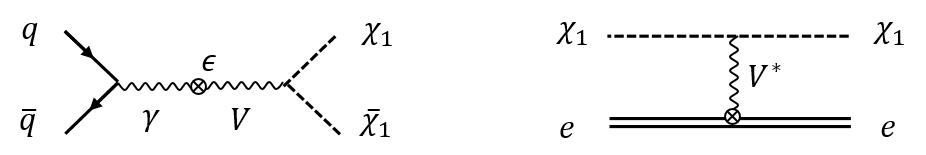
\includegraphics[width=\textwidth]{../graphics/DM_prod_detect}
\caption{\label{fig:dm_prod} Direct production of dark matter via the vector portal (left panel) and DM-electon elastic scattering (right panel)}
\end{figure}
We are particularly interested in sub-GeV-range DM coming from the decay of $on$-shell $V$ throughout this section. Therefore, the dominant production mechanism is the Drell-Yan process via dark photon $s$-channel exchange (see the left panel of figure~\ref{fig:dm_prod}):
\begin{equation}
p + N \rightarrow V \rightarrow \chi_1 \bar \chi_1 \,.
\end{equation}
The cross section for production of the dark matter is then written as
\begin{equation}
\sigma(p + N \rightarrow V \rightarrow \chi_1 \bar \chi_1) = \sigma(pN\rightarrow V)\times {\rm Br}(V\rightarrow \chi_1 \bar \chi_1)\,.
\end{equation}
We can express the differential cross-section as a function of the DM laboratory-frame energy, $E_{\chi_1}$, and the angle
between its laboratory-frame momentum and the beam direction, $\theta$:
\begin{equation}
\frac{d\sigma(pN\rightarrow V\rightarrow \chi_1 \bar \chi_1)}{dE_{\chi_1}d\cos\theta} 
= \frac{\delta(x, \cos\theta)}{\delta(E_{\chi_1}, \cos\theta)}\cdot \frac{d\sigma(pN\rightarrow V)}{dx}\cdot {\rm Br}(V\rightarrow \chi_1 \bar{\chi}_1)\cdot g(\cos\theta),
\end{equation}
where the first factor on the right-hand side is the Jacobian associated with the above variable change. The
function $g$ describes the angular distribution of the DM in the $V$ rest frame and $x$ is associated with parton distribution function (PDF).  The parton distribution function (PDF) $f_{q/p(n)} (x)$ ) gives the probability of extracting the quark $q$ with momentum fraction $x$ from a
proton (neutron), see ref.~\cite{deNiverville:2012ij} for detail information about PDF.\\
Once DM is produced, its detection can be done in the ND by elastic electron scattering via neutral current interactions, as depicted in the right panel of figure~\ref{fig:dm_prod}.
The electron scattering differential cross section takes the form
\begin{equation}
\frac{d\sigma_{{\chi_1}e}}{dE_{e}} 
= 4\pi \epsilon^{2}\alpha_{11}\alpha \frac{2m_{e}E_{\chi_1}^{2} - (2m_{e}E_{\chi_1} + m_{\chi_1}^{2})(E_e-m_{e})}{(E_e^{2}-m_{\chi_1}^{2})(m_{V}^{2}+2m_{e}E_{e}-2m_{e}^{2})^{2}}\,,
\end{equation}
where $E_{e}$ is the electron recoil  energy, $E_{\chi_1}$ is the incoming DM $\chi_1$ energy, and $\alpha_{11}$ is the fine structure constant between the dark photon and dark matter particles.
A signal event involves only a recoil electron in the final state. Scattering angle and energy of such a scattered electron can be reconstructed in the ND, so we consider these two kinematic observables as discriminators between our signal and various backgrounds.
\subsubsection{Background consideration}
 The background to the process showing the right panel of figure~\ref{fig:dm_prod} consists of any processes involving an electron recoil. As the ND is located near the surface, background events, in general, can be induced by cosmic rays as well as neutrinos generated from the beam. However, we do not consider the former possibility in this analysis because it is expected that a significant amount of cosmic background can be vetoed by the trigger and timing information of the injection beam. 
The major background will be neutrinos stemming from the proton beam. 
%A majority of such neutrinos are $\mu$-flavored, followed by electron-flavored. 
%The $\nu_\mu$ can induce a signal-like event via a neutral current (N.C.) interaction, whereas the $\nu_e$ give rise to a single electron through both charged current (C.C.) and N.C. interactions. 
%In general, a C.C.-induced scattering cross section is larger than the corresponding N.C.-induced, so the contributions from $\nu_\mu$ and $\nu_e$ should be comparable. 
%Another possible source is $\nu_e$-initiated C.C. events accompanying a nucleus recoil soft enough to be missed. Such a quasi-elastic process comes with a sizable scattering cross section, so that even a small missing probability would result in a considerable event rate. 

We take $\nu$-electron N.C. events just for simplicity. 
Although an accurate data analysis requires to include all non-negligible background sources, in this ``preliminary'' study we rather illustrate the overall flow of relevant procedures, leaving a more dedicated analysis to the future.
Nevertheless, we believe that our work here  not only give a guideline and some insights for future actual analyses but allow us to develop the intuition on the associated experimental sensitivities which DUNE would achieve.
\subsubsection{Simulation and event selection}
To generate event data of dark matter produced in the DUNE target, we
utilize the \texttt{MG5@aMC} particle event generation software~\cite{Alwall:2014hca}. 
For simplicity, we import 
%We first import the Light Dark Matter model, 
the light dark matter model in eq.~\eqref{eq:lagrangian} for fermionic dark matter. We are only concerned with the direct production of dark matter via proton collision, and therefore analyze  the $p + p \rightarrow \chi_1 + \bar{\chi_1}$ process. 
%Since we wish to simulate a proton beam on a proton fixed target, we choose the beam to be composed of protons with one beam at the desired beam energy and the other at the proton mass.
%The resulting dark matter energy (left panel) and angular distributions (right panel) at the target location are shown in figure~\ref{fig:DM_prod}.
%\begin{figure}[t]
% \centering
% 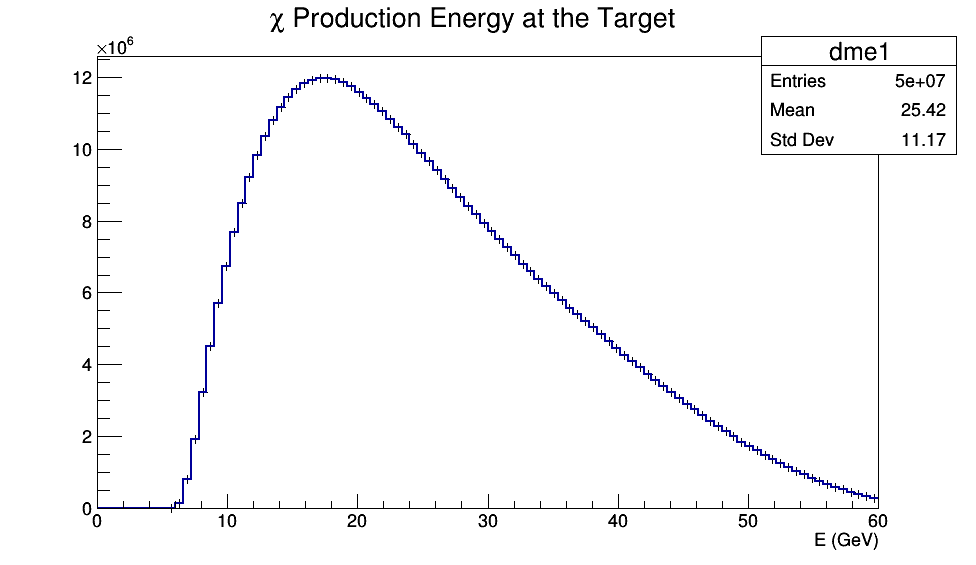
\includegraphics[width=8.0cm,height=6.0cm]{DM_ProdE}
% 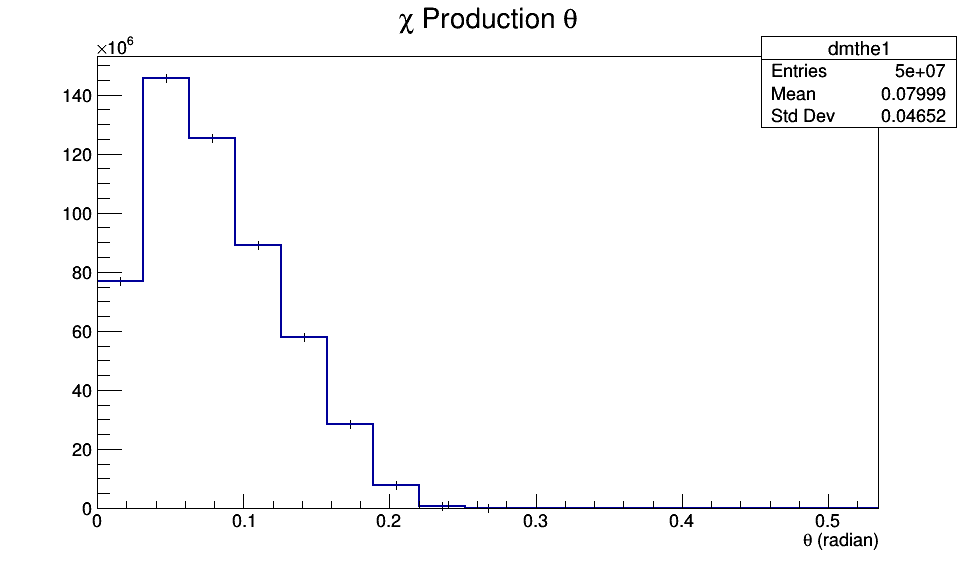
\includegraphics[width=8.0cm,height=6.0cm]{DM_theta}
% \caption{\label{fig:DM_prod} Dark matter energy (left panel) and theta distribution (right panel) at the target location shown, respectively. 
%The spectrum is for $m_{\chi_1}=2$ GeV, $m_{V}=6$ GeV, $\epsilon=10^{-3}$, and $\alpha_{11}=0.5$, respectively. }
% \end{figure}
% Neutrino flux at the ND location is shown in figure~\ref{fig:NuE}. The neutrino flux is weighted at the ND location. 
%
% \begin{figure}[!h]
% \centering
% 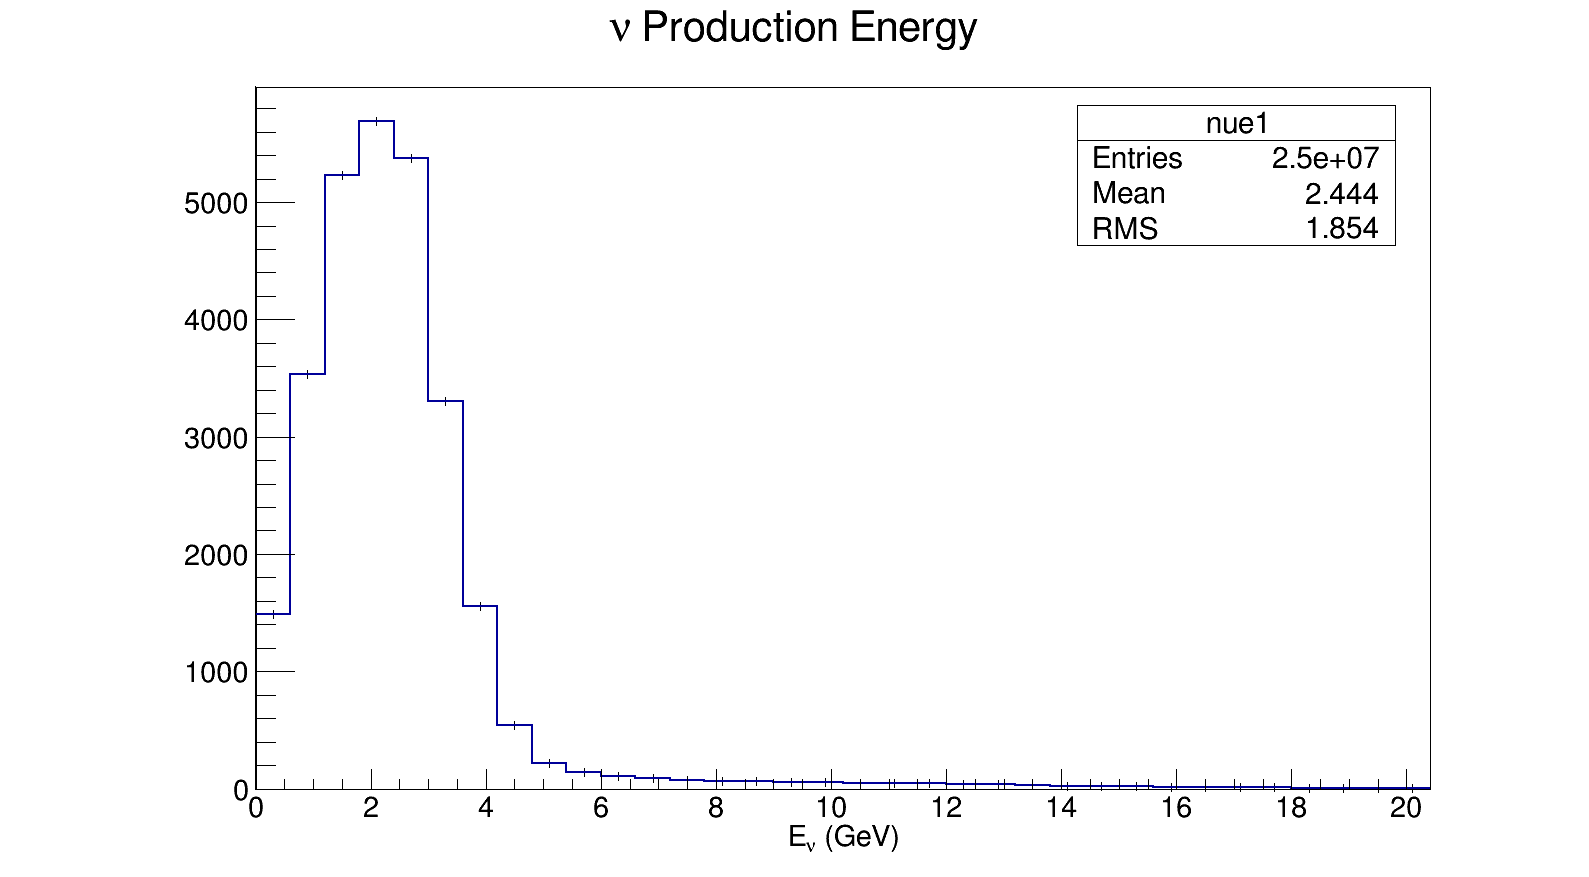
\includegraphics[width=8.0cm,height=6.0cm]{Nu_prodE}
% \caption{\label{fig:NuE} Neutrino flux at the ND location.}
% \end{figure}
% \begin{table}[h]
%   \begin{landscape}
 %   \begin{center}
        %\caption{Specifications of LTE}
        %\label{tab:table1}
        %\begin{adjustbox}{max width=\textwidth}
  %      \resizebox{0.8\textwidth}{!}{
   %         \begin{tabular}{ | l  l |} 
    %           \hline 
     %          ND  properties& Values\\
      %         \hline
       %        Near detector dimension & 4m(W) x 3m(H) x 5m(L) ($\approx$ 85 tons)\\ 
        %        Near detector location from target & 570 m \\
         %      Detector efficiency& 85$\%$\\ 
          %      Energy resolution& $\frac{5\%}{\sqrt{E}}$ \\  
           %     Beam power & 1.2MW with 50$\%$ duty cycle \\ \hline
            %\end{tabular} }
            %\end{adjustbox} 
        %\end{center}
        %\caption{\label{tab}ND properties used for the analysis }
    %\end{table} 
    
    The next step in our calculations is to reweight the neutrino and dark
matter distributions so that they correspond to the correct number of protons
on target for the DUNE experiment. 
 \begin{figure}[!h]
 \centering
 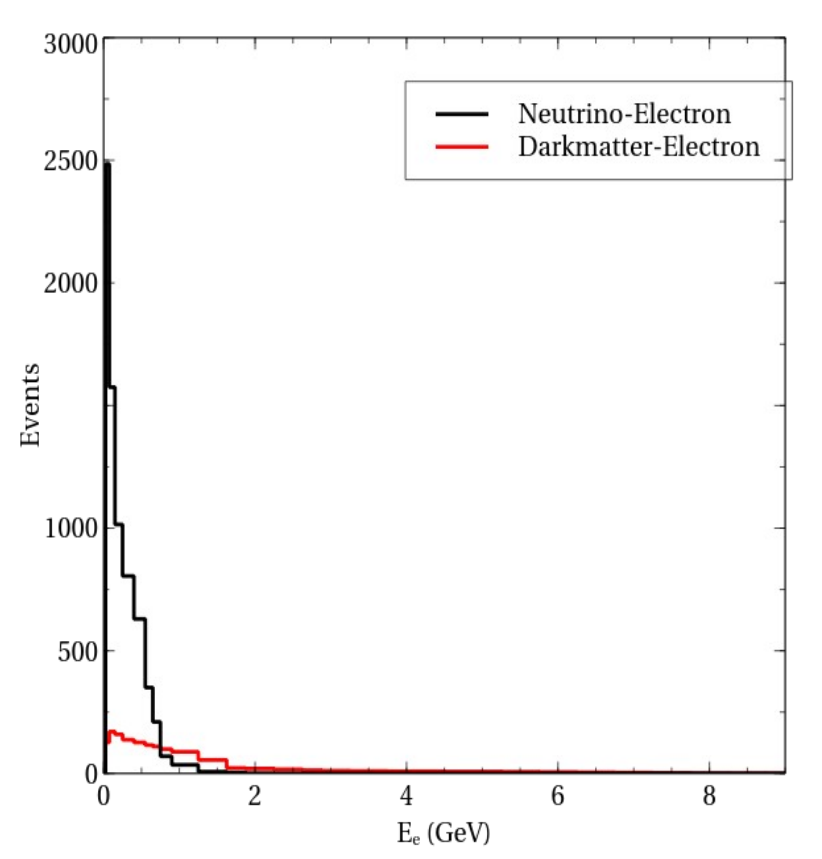
\includegraphics[width=8.0cm,height=6.0cm]{ScatteredE}
 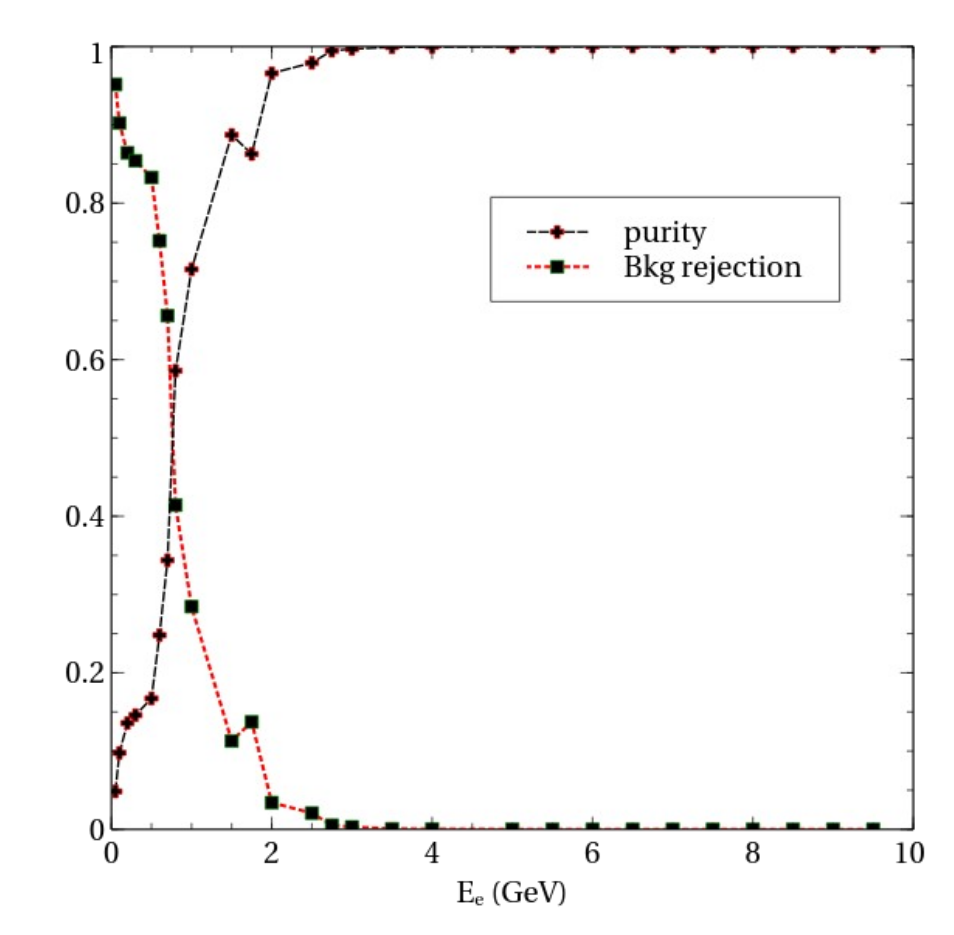
\includegraphics[width=8.0cm,height=6.0cm]{Purity}
 \caption{\label{fig:scatter_E} Scattered energy (left) and purity (right) shown for $m_{\chi_1}=2$ GeV, $m_{V}=6$ GeV, $\epsilon=10^{-3}$, and $\alpha_{11}=0.5$, respectively. }
 \end{figure}
The scattered energy distribution for both the signal and background events are shown in the left panel of figure~\ref{fig:scatter_E}.
The background rate (i.e., $\nu$-electron scattered events) is very large at low energies (below $\sim 1$ GeV), whereas signal events display a harder spectrum. 
As mentioned earlier, we have used two kinematic variables, the recoil energy and recoil angle, in order to reject background events. 
We introduce two dynamical variables as purity and background rejection for the event selection. 
Purity is defined as the ratio of the number of signal events over the total number of events for each energy and angular bin. 
Similarly, background rejection is defined as the ratio between number of background events over the total number of events. 
We calculate sensitivity ($\chi^{2}$) for each energy and theta bins, and maximize the $\chi^{2}$ when purity is greater or equal to background ratio (rejection). The right panel of figure~\ref{fig:scatter_E} reports the purity and background rejection vs energy.
\subsubsection{Sensitivity calculation and results}
The sensitivity results for the analysis were generated for the dark sector parameters  $m_{V}=3m_{\chi_1}$, $\alpha_{11}=0.5$. 
We have calculated the $\chi^{2}$ sensitivity in the parameter space $Y$ vs $m_{\chi_1}$, where 
\begin{equation}
Y\equiv\epsilon^{2}\alpha_{11} (\frac{m_{\chi_1}}{m_{V}})^{4}
\end{equation}
is a dimensionless parameter that controls the dark matter annihilation cross section and in turn the thermal relic abundance. 
For the $\chi^{2}$ calculation, we take into account smearing energy in the  near detector.
The smearing and all the detector parameters are given in table~\ref{tab}. 
To smear energy, we use the predicted smearing of 5$\%$ presented in the DUNE CDR \cite{Acciarri:2015uup} with a Gaussian resolution function.
%\begin{table}[h]
%   \begin{landscape}
 %   \begin{center}
        %\caption{Specifications of LTE}
        %\label{tab:table1}
        %\begin{adjustbox}{max width=\textwidth}
  %      \resizebox{0.4\textwidth}{!}{
    %        \begin{tabular}{ | l  l |} 
     %          \hline 
      %         Uncertainties& Values\\
       %        \hline
        %      Flux & 20$\%$\\ 
         %       Cross-section & 10$\%$ \\
          %     Scattering angle of electron& 5$\%$\\ 
           %     Detector systematic& 5$\%$ \\  \hline
            %\end{tabular} }
            %\end{adjustbox} 
        %\end{center}
        %\caption{\label{tab2}Systematic uncertainties used for sensitivity calculation }
    %\end{table} 
%\begin{equation}
%R_{E} = \frac{1}{\sqrt[]{2\pi}\sigma}exp\big[-%\frac{(E_{m} - E_{t})^{2}}{2{\sigma}^{2}}\big],
%\end{equation}
%where $E_{m}$ and $E_{t}$ are the measured and true energies and $\sigma$ is smearing width given in table~\ref{tab}.
%The $\chi^{2}$ with the systematic uncertainties is defined as
%\begin{equation}
%\chi^{2}(\xi_{k}) = \sum_{i}\left(\frac{\left\{N^{\rm th}_{i} - N^{\rm ex}_{i} + \sum(C_{k}\xi_{k})\right\}^{2}}{N^{\rm ex}_{i}}\right)\,,
%\end{equation}
%where $N^{\rm th}$ and $N^{\rm ex}$ are given by
%\begin{equation}
%N^{\rm th}= N^{\rm sig} + N^{\rm bkg},\quad N^{\rm ex} = N^{\rm bkg}. 
%\end{equation}
%Here the $C_{k}$ are the coefficients of the systematic uncertainties  and $\xi_{k}$ is the pull variable which minimizes the $\chi^{2}$ over the uncertainties.
%Finally, $\chi^{2}$ is marginalized over $\xi_{k}$.

%\subsection{Results}

The $\chi^{2}$ values are calculated for each set of two dark matter parameters ($Y$ vs $m_{\chi_1}$).
In Figure~\ref{fig:chisq}, with $m_{V} = 3m_{\chi}$ and $\alpha_{11}=0.5$,  the 90$\%$ C.L  values for the dimensionless DM annihilation
cross section parameter $Y = \epsilon^{2}\alpha_{11} (m_{\chi}/m_{V})^4$ plotted both 80 GeV and 120 GeV proton energy (left) compared to different experimental exclusion regions (right).
 \begin{figure}[t]
 \centering
 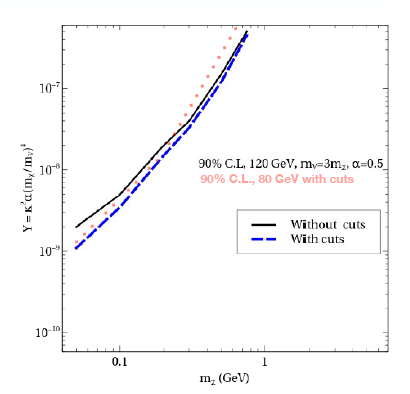
\includegraphics[width=8.0cm,height=6.0cm]{image1}
 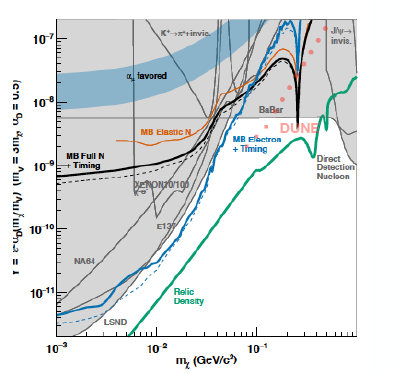
\includegraphics[width=8.0cm,height=6.0cm]{image2}
 \caption{\label{fig:chisq} Left: 90$\%$ Confidence level limit for Y as a function of $m_{\chi}$, assuming $\alpha_{11}=0.5$ and $m_{V} = 3m_{\chi}$ at the DUNE ND. 
The red dotted (blue dashed) line shows the expected sensitivity for 80 GeV (120 GeV) proton energy. 
The chosen parameters are $\alpha_{11}=0.5$ and $m_{V}= 3m_{\chi_1}$.
Right: The sensitivity with the other experiments.}
 \end{figure}

\subsection{Cosmic Frontier Search: DUNE FD and ProtoDUNE \label{sec:FD}}

\subsubsection{Flux of boosted dark matter \label{sec:flux}}

As we mentioned in the Introduction, we look at an annihilating two-component DM scenario~\cite{Belanger:2011ww} in this study. 
The heavier DM (denoted $\chi_0$) plays a role of cosmological DM and pair-annihilates to a pair of lighter DM particles (denoted $\chi_1$) in the universe today. 
The expected flux near the Earth is given by~\cite{Agashe:2014yua, Giudice:2017zke, Kim:2018veo}
\bea 
\mathcal{F}_1= & 1.6 \times 10^{-6} {\rm cm}^{-2}{\rm s}^{-1}\times \left( \frac{\langle \sigma v\rangle_{0\rightarrow 1}}{5\times 10^{-26}{\rm cm}^3{\rm s}^{-1}}\right) 
 \times \left( \frac{10\, {\rm GeV}}{m_{\chi_0}}\right)^2\,,
\label{eq:flux}
\eea
where $m_{\chi_0}$ is the mass of $\chi_0$ and $\langle \sigma v\rangle_{0\rightarrow 1}$ stands for the velocity-averaged annihilation cross section of $\chi_0\bar{\chi}_0 \to \chi_1\bar{\chi}_1$ in the current universe.
To evaluate the reference value shown as the first prefactor, we take $m_{\chi_0} = 10$ GeV and $\langle \sigma v\rangle_{0\rightarrow 1}=5\times 10^{-26}{\rm cm}^3{\rm s}^{-1}$, the latter of which is consistent with the current observation of DM relic density assuming $\chi_0$ and its anti-particle $\bar{\chi}_0$ are distinguishable. 
In order to integrate all relevant contribution over the entire galaxy, we assume the Navarro-Frenk-White (NFW) DM halo profile~\cite{Navarro:1995iw, Navarro:1996gj}.
In this section, we assume the BDM flux with a $m_{\chi_0}$ dependence given by eq.~(\ref{eq:flux}) for the phenomenological analysis. 


\subsubsection{Experimental signatures}

The boosted dark matter, which is created, e.g., at the galactic center, reaches the DUNE FDs and ProtoDUNE detectors and scatters off either electrons or protons energetically. 
In this study, we focus on electron scattering signatures for illustration. 
%The search scheme to be described later on is straightforwardly applicable also to proton scattering, which will be mentioned wherever needed. 
%As can be seen from the Lagrangian [see eq.~\eqref{eq:lagrangian}], in an inelastic BDM ($i$BDM) signal event, $\chi_1$ scatters off an electron to a heavier state $\chi_2$ via the exchange of virtual dark photon. 
%The $\chi_2$ then decays back to $\chi_1$ and an electron-positron pair via an on-shell or off-shell dark photon depending on the mass spectrum. 
The overall process is summarized as follows:
\bea 
\chi_1 + e^- \to e^- + \chi_2 (\to \chi_1 + V^{(*)} \to \chi_1 + e^+ +e^-)\,,
\eea
and a diagrammatic description is shown in figure~\ref{fig:sig} where detector-visible particles are enclosed by a blue circle. 
Therefore, in the final state, there exist three visible particles which usually leave sizable ($e$-like) tracks in the DUNE and ProtoDUNE detectors.  
Note that we can replace $e^-$ in the left hand side and the first one in the right hand side of the above process to $p$ for $p$-scattering case.
In this case, the primary signature is quasi-elastic proton recoiling~\cite{pscattering} if the source of BDM is Galactic Center in the basic model in eq.~\eqref{eq:lagrangian}.

\begin{figure}[t]
\centering
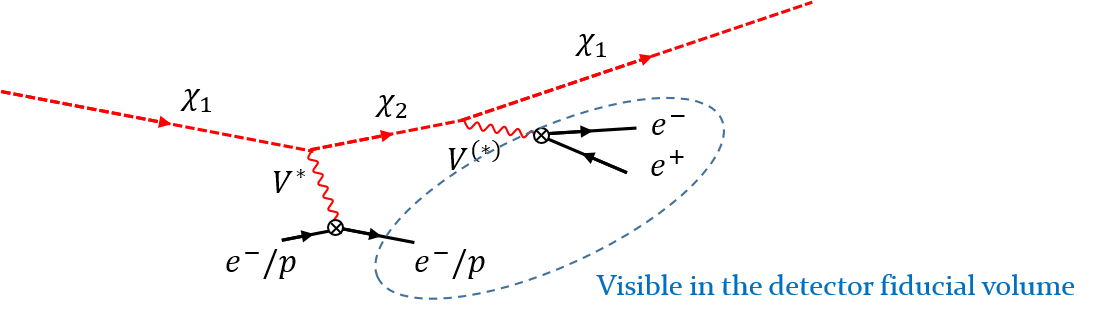
\includegraphics[width=6cm]{signature}
\caption{\label{fig:sig} The inelastic boosted dark matter signal under consideration.}
\end{figure}

%An interesting possibility for signal events is that the secondary particles, i.e., the $e^+e^-$ pair from the $\chi_2$ decay, may be displaced from the recoil electron. 
%If the mass spectrum allows $\chi_2$ to decay to $\chi_1$ and on-shell $V$, the $V$ can be long-lived with a small kinetic mixing parameter. 
%On the other hand, if $\chi_2$ undergoes a three-body decay process, it itself can be long-lived (see ref.~\cite{Giudice:2017zke} for more detailed discussion along these lines including the decay lengths of $\chi_2$ and $X$). 
%Once the two interaction points in a signal event are appreciably separated, it gets easier to distinguish it from potential background events. 
%Hence, signal isolation can benefit from this feature. 
%Moreover, we expect to correlate the two signatures due to the excellent ability of DUNE in correlating the directional, time, and distance between the two signatures.


\subsubsection{Background estimation}

As we have identified a possible $i$BDM signature, we are now in a position to discuss potential SM background events. 
%Due to the difference in the detector locations, it is more informative to split our discussion on the background estimates into two parts: one for the ProtoDUNE detectors and the other for the DUNE FDs. 
%For the {\it i}BDM signals, we can categorize the events by the type of the primary scattering signature ($e$- or $p$-scattering) and the secondary signature ($e^+ e^-$, $\mu^+ \mu^-$, $\pi^+ \pi^-$, etc.).
%Here, we focus on the possible background events which can mimic the $e$-scattering in the primary signature and $e^+ e^-$ in the secondary signature.

The biggest challenge in the search for BDM signals at ProtoDUNE is the fact that it involves surface-based detectors which suffer from an enormous amount of cosmic-ray backgrounds such as muons or neutrons.
%In the case of {\it i}BDM search, it is still rare for the cosmic-origin background events to mimic the signal events due to some distinctive features discussed in the preceding section.
%Nevertheless, we contemplate possible signal-faking scenarios~\cite{Chatterjee:2018mej}, mostly stemming from the cosmic muons whose estimated rate is $\sim 4 \times 10^{11}$ per year in each detector.
The most plausible scenario in which a cosmic muon might mimic the signal is as follows: a muon i) enters the fiducial volume without leaving a track, i.e., ``sneaks-in'', ii) emits a hard photon which converts into an $e^+ e^-$ pair, and iii) starts to leave a visible track resulting in a signal-like event shape, iv) which appears electron-like.
%In summary, these cosmic muons mimicking the {\it i}BDM signal are coming from the imperfect reconstruction of muons.
%The probability that a muon satisfies the second criterion is theoretically given by a phase-space suppression factor, $\alpha/\pi \approx 2 \times 10^{-3}$~\cite{Tanabashi:2018oca}. 
For the criteria i) and iv), we conservatively take the upper limits 0.1\% and 1\%, respectively, from some preexisting dedicated studies of muon reconstruction efficiency under a similar LArTPC-detector environment~\cite{MicroBooNEmuon, Acciarri:2016sli}.
If we achieve $\sim 0.6\%$ of suppression power in the criterion iii), the number of the corresponding background events can be fewer than $\sim 100$ per year at the ProtoDUNE detectors.
%Indeed, a dedicated analysis would allow us to veto these rare possibilities by a few orders of magnitude.
%Nevertheless, we will present the experimental sensitivities assuming a total of 100 background events per year at the ProtoDUNE detectors in order to highlight the fact that the ProtoDUNE detectors are powerful machines in searching for the {\it i}BDM signals even under a challenging circumstance.
%We have estimated and checked that the other subleading backgrounds, e.g., di-muon simultaneous scattering, muon-initiated deep inelastic scattering, and the neutrino-initiated deep inelastic scattering, are negligible (i.e., $< 0.1$ per year per detector)~\cite{Chatterjee:2018mej}. 

%The event selection scheme described above might suffer from systematics through background modeling. 
%A possible way to circumvent this issue is to utilize high-quality directional information available at LArTPC detectors. 
%Considering the fact that most of such events come from the sky, we regard the Earth as a shield for cosmic-induced backgrounds~\cite{Kim:2018veo}.
%In the case of {\it e}BDM search at ProtoDUNE, we can enhance the signal-to-background ratio using the Earth as a shielding material of the background~\cite{Kim:2018veo}. 
%To apply this so-called {\it Earth Shielding} idea to the $i$BDM search at ProtoDUNE detectors, we restrict ourselves to collect events coming through the Earth, %from the opposite side of the detector location, 
%i.e., up-going events. 
%Relevant signal events essentially come out of the ground and leave appreciable tracks from which the source direction can be inferred.
%We have found that about 70\% (50\%) out of 1-year data originating from the galactic center (the Sun) can be used in the search for BDM signals (see ref.~\cite{Kim:2018veo} for more details on the Earth Shielding effect).
%Actually, the Sun is a good candidate source of BDM through annihilation of heavier DM captured by the Sun although we are focusing on BDM from the galactic center in the study.
%We refer to refs.~\cite{Berger:2014sqa, Kong:2014mia, Alhazmi:2016qcs} for detailed description on DM capture, annihilation, energy loss inside the Sun, and the final solar BDM flux. 
%Then, the remaining background events are the quasi-elastic neutrino scattering which can reduced by considering the direction of the BDM sources. 
%For the {\it e}BDM signals coming from the GC, we estimate about 14.1 (0.95) background events exist in the total fiducial volume of the SP and DP detectors at ProtoDUNE using the Earth-Shielding method taking the data within 30$^\circ$ cone (whole sky) around the Galactic Center.

When it comes to the DUNE FDs located $\sim 1480$ m deep underground, the cosmic-induced background discussed earlier is not an issue any more. 
%However, they come with $\sim 100$ times larger detector volume than the ProtoDUNE detectors, so that atmospheric neutrinos may induce events mimicking signal ones. 
The most plausible scenario is the production of multiple pions that subsequently decay to electrons, positrons, and neutrinos. 
Relevant channels are the resonance production and/or deep inelastic scattering (DIS) by the charged current $\nu_e$ or $\bar \nu_e$ scattering with a nucleon in the LAr target.
%we expect that the most the dominant background events of the {\it i}BDM signals are the multi-pions which subsequently decay into electrons, positrons, and neutrinos. 
%These multi-pions are produced from the resonance production or deep inelastic scattering (DIS) by the charged current $\nu_e$ or $\bar \nu_e$ scattering with a nucleon in LAr target.
%Note that the flux of $\nu_\tau$ is too small to yield a meaningful event rate, $\nu_\mu$-induced charged current events are accompanied by a muon which is absent in the signal event, and the neutrino-induced neutral current events are sub-dominant compared to the charged current events.
Summing up all the resonance production and DIS events which are not only induced by $\nu_e$ or $\bar \nu_e$ 
%whose energy is larger than 1 GeV, 
but relevant to production of a few pions, we find that the total number of multi-pion production events is at most $\sim 12$ kt$^{-1}$yr$^{-1}$ based on the neutrino flux in ref.~\cite{Honda:2015fha} and the cross section in ref.~\cite{Formaggio:2013kya}.
%However, we anticipate that the events with more than 3 pions or the two neutral pion (i.e., four $\gamma$'s) would be easily rejected in the LArTPC detectors, unless some of the tracks are missed.
In addition, the charged pions often leave appreciable tracks inside the detector so that the probability of misidentifying the $e^\pm$ from the decays of $\pi^\pm$ with the {\it i}BDM signal events would be very small.
Hence, we conclude that it is fairly reasonable to assume that almost no background events exist.
For the ProtoDUNE detectors with the fiducial mass of $\sim0.5$ kt, the expected total number of atmospheric neutrino-induced multi-pion events is at most $\sim 6$ yr$^{-1}$, which would be significantly reduced again due to the good pion tagging efficiency. 
Thus, no atmospheric neutrino-induced backgrounds are expected for the ProtoDUNE detectors.  


%For the {\it e}BDM signals in DUNE FD, the signal events look exactly same as the neutral current scattering of $\nu_e$.
%Hence, the directional cuts around the Galactic Center or the Sun play the key roles as in the analysis at SK~\cite{Kachulis:2017nci}.
%{\color{blue}
%(More to add here?)
%}


\subsubsection{Phenomenology}\label{Sec:Pheno}

We finally present the expected experimental sensitivities at ProtoDUNE and DUNE, in the searches for $i$BDM.
We closely follow the strategies illustrated in refs.~\cite{Giudice:2017zke, Chatterjee:2018mej, Kim:2018veo} in order to represent phenomenological interpretations. 

\begin{figure}[t]
\centering
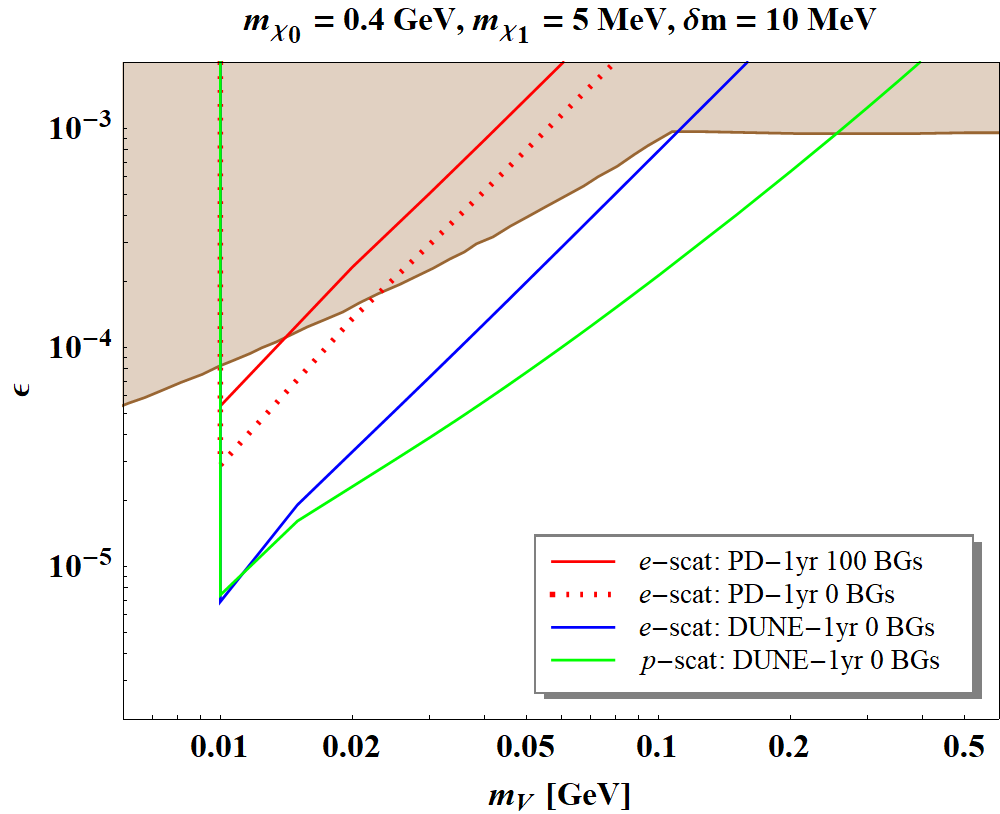
\includegraphics[width=6cm]{inv_PD_vs_DUNE} 
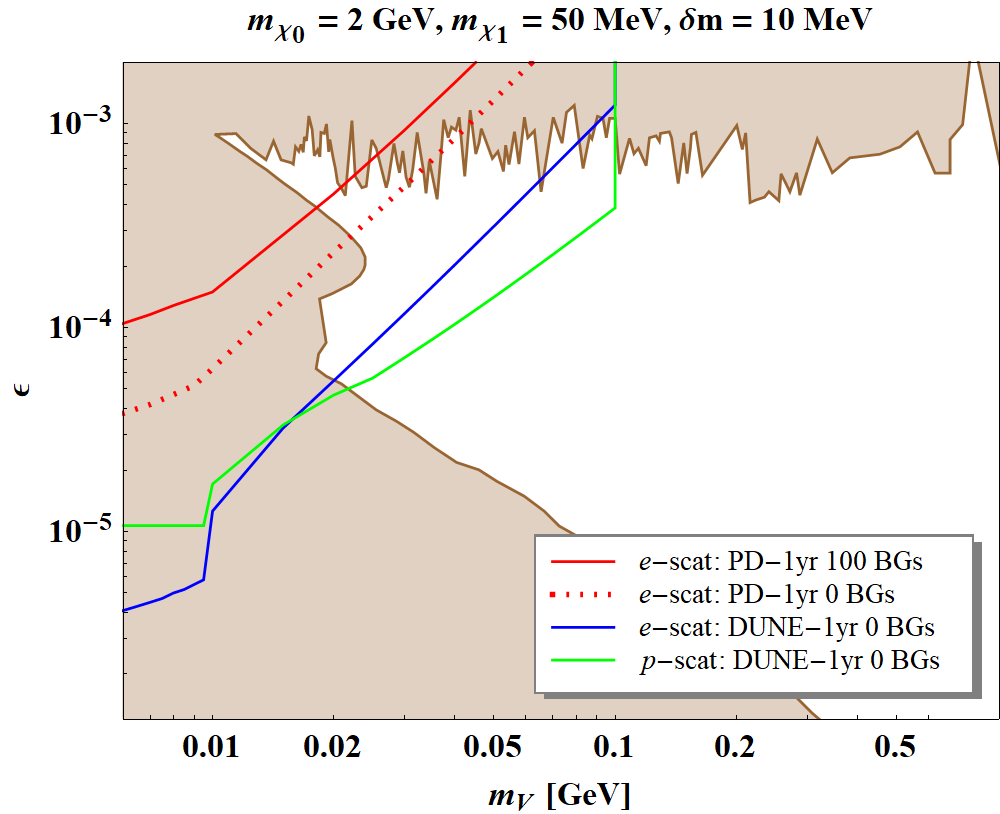
\includegraphics[width=6cm]{vis_PD_vs_DUNE} \\
\vspace{0.3cm}
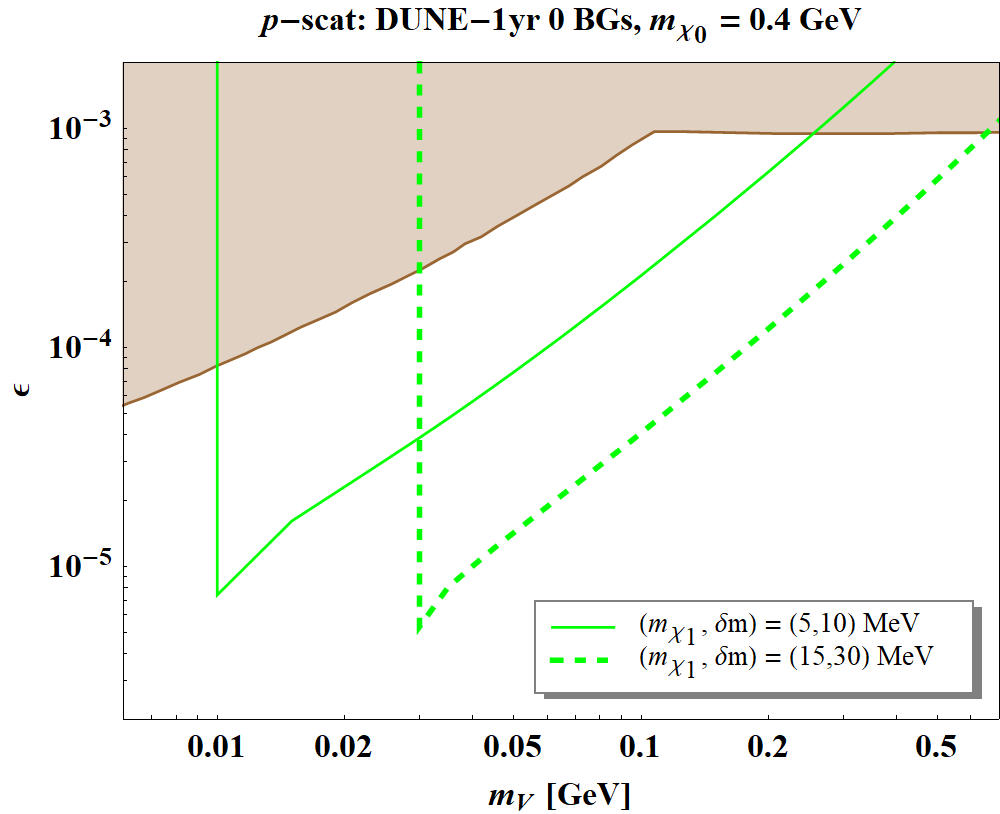
\includegraphics[width=6cm]{inv_DUNE_p-scatterings}
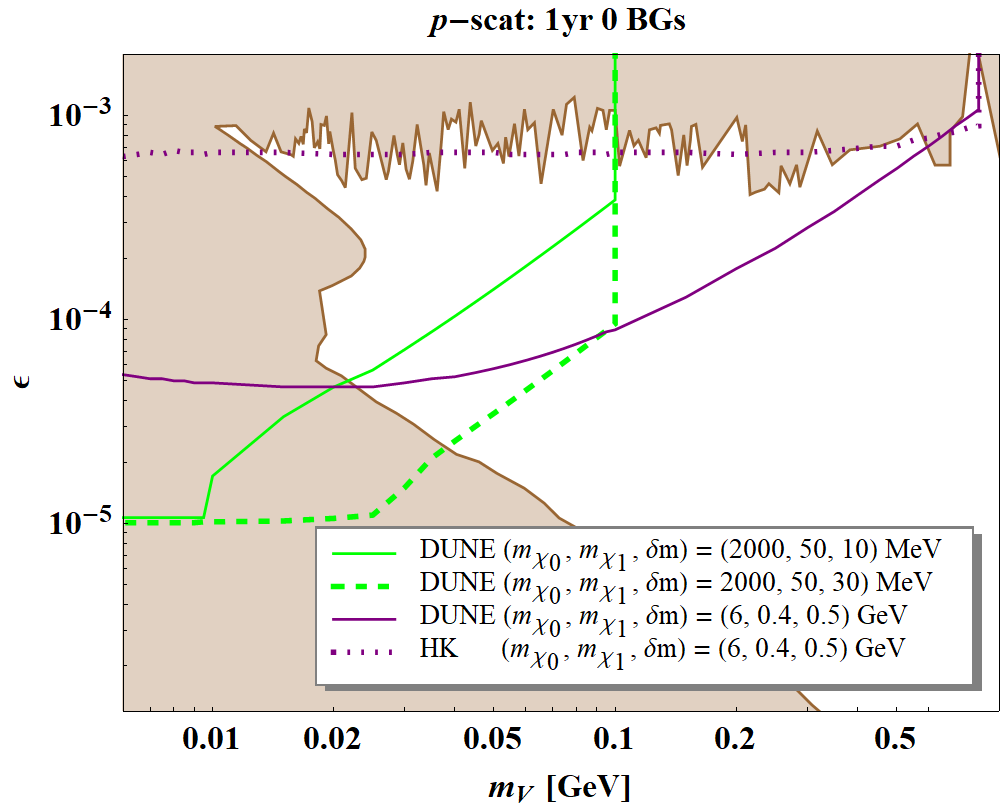
\includegraphics[width=6cm]{vis_DUNE_p-scatterings}
\caption{
The experimental sensitivities in terms of reference model parameters $m_V - \epsilon$ 
for $m_{\chi_0} = 0.4$ GeV, $m_{\chi_1} = 5$ MeV, and $\delta m = m_{\chi_2} - m_{\chi_1} = 10$ MeV (upper-left panel) and $m_{\chi_0} = 2$ GeV, $m_{\chi_1} = 50$ MeV, and $\delta m = 10$ MeV (upper-right panel).
The left panels are for Scenario 1 and the right ones are for Scenario 2.
The lower panels compare different reference points in the $p$-scattering channel.
See the text for the details.
\label{fig:darkphotonparameter} }
\end{figure}

%As the benchmark model in eq.~\eqref{eq:lagrangian} involves a dark photon, we first investigate the experimental sensitivity in terms of the standard $m_V\,-\,\epsilon$ space.
%Exclusion limits differ from the case of $m_V > 2m_{\chi_1}$ to the case of $m_V \le 2m_{\chi_1}$ (for which dark photon would decay invisibly and visibly, respectively, if it would be produced $on$-shell from the $\chi_2$ decay), so we perform two separate analyses, displaying the results for the former (latter) in the left (right) panel of figure~\ref{fig:darkphotonparameter}. 
%All our limits are reported at 90\% C.L. for a given background assumption. 
%The energy threshold for observing an electron (proton) with an angular resolution of $\sim 1^\circ$ ($\sim 5^\circ$) is set to 30 MeV throughout all the analyses in this study.
%In order to show the ability of ProtoDUNE and DUNE in searching for BDM signals, we first show the experimental sensitivities in terms of the parameters in the benchmark model described in Sec.~\ref{sec:model}. 

In displaying the results, we separate the signal categories such that
%--
\begin{itemize}
\item Scenario 1: $m_V > 2 m_{\chi_1}$, Experimental limits for $V \to$ invisible  applied.
\item Scenario 2: $m_V \le 2 m_{\chi_1}$, Experimental limits for $V \to e^+ e^-$ invisible  applied.
\end{itemize}
%--
%assuming BR($V \to \chi_1 \bar \chi_1$) = 1 for Scenario 1 and BR($V \to e^+ e^-$) = 1 for Scenario 2.
%Hence, we can apply the different experimental constraints ($V \to$ invisible~\cite{Banerjee:2017hhz} and $V \to e^+ e^-$~\cite{Banerjee:2018vgk}) for the above two scenarios.
%Note that the boundary dividing the Scenario 1 and 2 can be $m_V = m_{\chi_1} + m_{\chi_2} = m_{\chi_1} (1 + \delta m)$ in a special scenario that the off-diagonal gauge coupling $g_{12}$ in eq.~(\ref{eq:lagrangian}) is maximized while the diagonal coupling $g_{11}$ is turned-off, as stated in ref.~\cite{Giudice:2017zke}.
%If $V$ is produced on-shell in Scenario 1, the secondary signature is invisible and hence the whole signal will be categorized as elastic BDM.

%In Scenario 1, we first study the electron scattering channel, taking $m_{\chi_0} = 0.4$ GeV, $m_{\chi_1} = 5$ MeV, and $\delta m = m_{\chi_2} - m_{\chi_1} = 10$ MeV as a reference point, and then show the result in the upper-left panel of figure~\ref{fig:darkphotonparameter}.
%As reference parameters, we choose $m_0 = 0.4$ GeV, $m_1 = 5$ MeV, and $\delta m = m_2 - m_1 = 10$ MeV in the top-left panel of Fig.~\ref{fig:darkphotonparameter} where we show the sensitivities in terms of the mass of the new gauge boson $m_X$ and the kinetic mixing parameter $\epsilon$ when the dark photon dominantly decays to the pair of dark matter $X \to \chi_1 \bar \chi_1$, i.e., invisible particles. 
The brown shaded region shows the latest limits set by various experiments such as the fixed target experiment NA64 at the CERN SPS and the B-factory experiment BaBar~\cite{Banerjee:2017hhz}.
The red solid (dotted) line describes the experimental sensitivity~\footnote{This is defined as the boundary of parameter space which can be probed by the dedicated search in a given experiment at 90\% C.L., practically obtained from eq.~(\ref{eq:MIsensitivity}).} at ProtoDUNE under the assumption of 100 (zero) background events. 
The associated exposure is 470 t$\cdot$yr, i.e., a total fiducial volume of 470 t times 1-year running time. 
The corresponding DUNE result is represented by the blue solid line with 40 kt$\cdot$yr exposure and a zero background assumption. 
%In the panel, we show the experimental sensitivities of $e$-scattering signal at ProtoDUNE assuming the number of background is 100 (red solid line) and zero (red dotted line), when the detector is exposed in 1 year.
%Then, the sensitivities at DUNE is shown in blue solid line under zero-background assumption.
For comparison, we also show the sensitivities of DUNE to the $p$-scattering signal as a green solid line. 
%We emphasize that the low energy threshold for observing the proton recoiling signal in LArTPC allows DUNE to possess sensitivity remarkable enough to explore $p$-scattering $i$BDM signals, whereas such sensitivity is not in general expected in the experiments utilizing Cherenkov light detectors due to high proton threshold energy.
%In addition, ProtoDUNE and DUNE have enough sensitivities to the parameter set where $m_0$ is as low as 400 MeV, which is impossible in the experiments using the Cherenkov light detectors in general. 

Inspired by this potential of searching for the proton scattering channel, we study another reference parameter and compare it with the original one in the lower-left panel of figure~\ref{fig:darkphotonparameter}. 
We see the reachable $\epsilon$ values rise, as $m_V$ increases. 
%However, the plot suggests that assumptions of different reference points allow to probe different regions of parameter space. 
%Since the proton is much heavier than typical $\chi_1$ of interest, large $\delta m$ values are kinematically accessible. 
%Indeed, for the case where $\chi_2$ decays through a three-body process, a large $\delta m$ reduces the decay length of $\chi_2$, offsetting the effect from a small $\epsilon$~\cite{Giudice:2017zke}. 
%Therefore, a decent level of signal acceptance is retained even with small $\epsilon$ values, unlike in the electron-scattering channel. 

For Scenario 2 (the right panels of figure~\ref{fig:darkphotonparameter}), we choose a different reference parameter set: $m_{\chi_0} = 2$ GeV, $m_{\chi_1} = 50$ MeV, $\delta m = 10$ MeV. 
The current limits (brown shaded regions), from various fixed target experiments, B-factory experiments, and astrophysical observations, are taken from ref.~\cite{Banerjee:2018vgk}.
%Again we see that ProtoDUNE (red lines) and DUNE (blue and green lines) can cover a wide range of unexplored parameter space. The kink at $m_V=10$ MeV arises because $\chi_2$ decays to an {\it on}-shell dark photon below this mass, so that resulting kinematics and dynamics change. 

%Being aware that large $m_{\chi_0}$ (or equivalently energy of the boosted $\chi_1$) values allow even Cherenkov detectors to have signal sensitivity, we compare the coverages of DUNE and Hyper Kamiokande in the $p$-scattering channel for $m_{\chi_0}=6$ GeV~\cite{DUNEfar}. The results are shown in the lower-right panel of figure~\ref{fig:darkphotonparameter}. 
%Here we assume one-year running time corresponding to 40 kt$\cdot$yr and 380 kt$\cdot$yr exposure for DUNE and Hyper Kamiokande, respectively. 
%We see that the sensitivity of DUNE to the $p$-scattering process is about an order of magnitude better due to a lower proton threshold energy and the great particle identification of LArTPC detectors, although the volume is about 10 times smaller.

%Due to its excellent ability of identifying the particles with relatively low threshold energies in LArTPC, the experimental sensitivities to $p$-scattering can probe about two orders of magnitude wider parameter region, compared to the current limits, as shown with the green solid lines in the top panels of Fig.~\ref{fig:darkphotonparameter}.
%For comparison, we show the coverage of $p$-scattering {\it i}BDM signals both in DUNE and Hyper Kamionkande in the bottom panels of Fig.~\ref{fig:darkphotonparameter}.
%We see the sensitivity of DUNE to $p$-scattering process is about an order of magnitude better although the volume is about 1/5.

We next discuss model-independent experimental sensitivities. 
The experimental sensitivities are determined by the number of signal events excluded at 90\% C.L. in the absence of an observed signal.
The expected number of signal events, $N_{\rm sig}$, is given by
\begin{align}
N_{\rm sig} = \sigma_\epsilon \mathcal F A(\ell_{\rm lab}) t_{\rm exp} N_T\,,
\label{eq:NS}
\end{align}
where $T$ stands for the target that $\chi_1$ scatters off, $\sigma_\epsilon$ is the cross section of the primary scattering $\chi_1 T \to \chi_2 T$, $\mathcal F$ is the flux of $\chi_1$, $t_{\rm exp}$ is the exposure time, and $A(\ell_{\rm lab})$ is the acceptance which is defined as 1 if the event occurs within the fiducial volume and 0 otherwise.
Here we determine the acceptance for an $i$BDM signal by the distance between the primary and secondary vertices in the laboratory frame, $\ell_{\rm lab}$, so $A(\ell_{\rm lab}) = 1$ when both the primary and secondary events occur inside the fiducial volume. (Given this definition, obviously, $A(\ell_{\rm lab}) = 1$ for elastic BDM.)
Note that our notation $\sigma_\epsilon$ includes additional realistic effects from cuts, threshold energy, and the detector response, hence it can be understood as the fiducial cross section.

The 90\% C.L. exclusion limit, $N_s^{90}$, can be obtained with a modified frequentist construction~\cite{cls1,cls2}. We follow the methods in refs.~\cite{Dermisek:2013cxa,Dermisek:2014qca,Dermisek:2016via} where the Poisson likelihood is assumed. 
An experiment becomes sensitive to the signal model independently if $N_{\rm sig} \ge N_s^{90}$.
Plugging eq.~\eqref{eq:NS} here, we find the experimental sensitivity expressed by %the following inequality
\begin{align}
\sigma_\epsilon \mathcal F \ge \frac{N_s^{90}}{A(\ell_{\rm lab}) t_{\rm exp} N_T}\,. 
\label{eq:MIsensitivity}
\end{align}
Since $\ell_{\rm lab}$ differs event-by-event, we take the maximally possible value of laboratory-frame mean decay length, i.e., $\bar{\ell}_{\rm lab}^{\rm max} \equiv \gamma_{\chi_2}^{\max} \bar{\ell}_{\rm rest}$ where $\gamma_{\chi_2}^{\max}$ is the maximum boost factor of $\chi_2$ and $\bar{\ell}_{\rm rest}$ is the rest-frame mean decay length. 
We emphasize that this is a rather conservative approach, because the acceptance $A$ is inversely proportional to $\ell_{\rm lab}$.
We then show the experimental sensitivity of any kind of experiment for a given background expectation, exposure time, and the number of targets, in the plane of $\bar{\ell}_{\rm lab}^{\rm max} - \sigma_\epsilon \cdot \mathcal F$. 
The left panel of figure~\ref{fig:modelindependent} demonstrates the expected model-independent sensitivities at several experiments. 
The red (orange) line is for the ProtoDUNE detectors with the assumptions of 100 (zero) background events and 470 t$\cdot$yr exposure, while the green (blue) is for the DUNE FDs with a background-free assumption and 20 (40) kt$\cdot$yr exposure.

\begin{figure}[t]
\centering
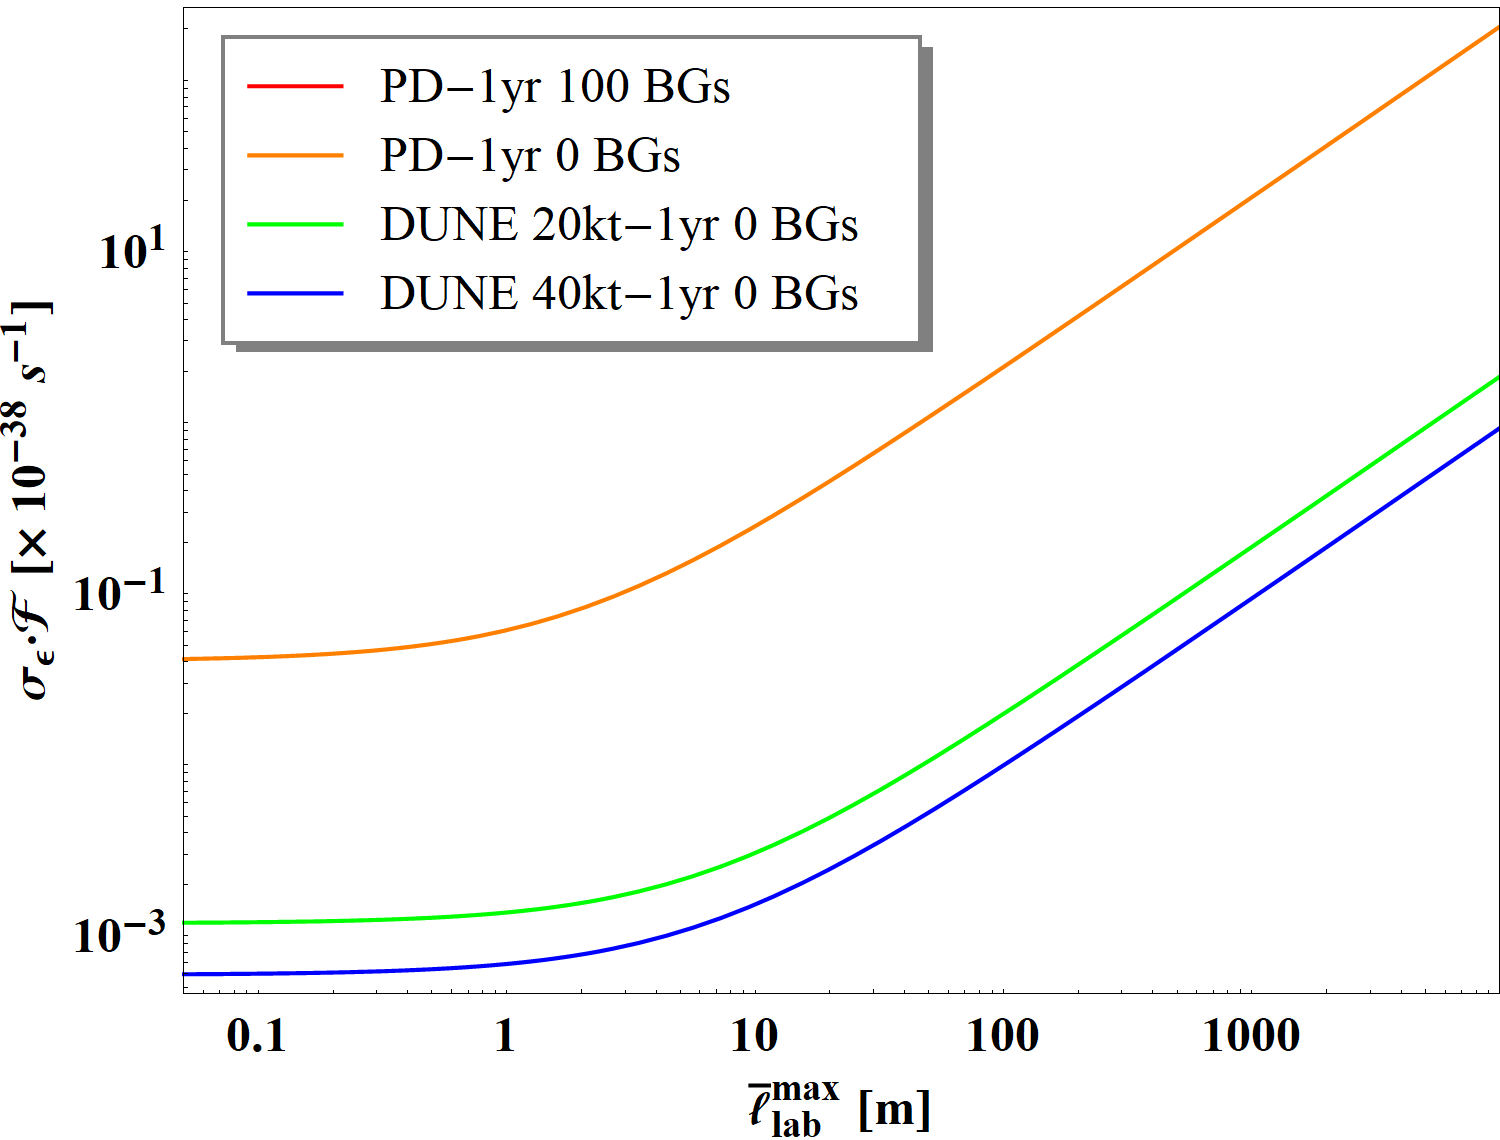
\includegraphics[width=6cm]{SigmaFluxVslMaxLab_TotalOnly}
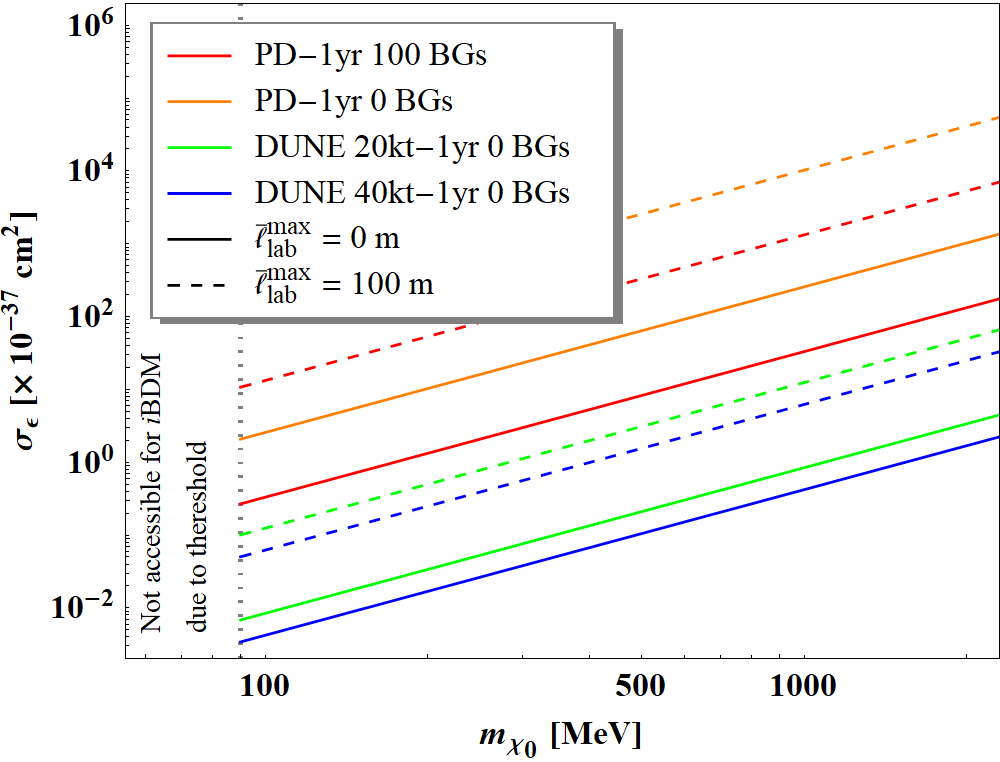
\includegraphics[width=6cm]{SigmaVsE1}
\caption{
Left: model independent experimental sensitivities of $i$BDM search in $\bar{\ell}_{\rm lab}^{\rm max} - \sigma_\epsilon \cdot \mathcal F$ plane. 
The reference experiments are ProtoDUNE with 100 background (red), zero-background (orange) assumption for 1-year time exposure, DUNE 20kt (green), and DUNE 40kt (blue) with zero-background assumption for 1-year time exposure. 
Right: Experimental sensitivities of $i$BDM search in $m_{\chi_0} - \sigma_\epsilon$ plane. The sensitivities for $\bar{\ell}_{\rm lab}^{\rm max} = 0$ m and 100 m are shown as solid and dashed lines for each reference experiment in the left panel.
\label{fig:modelindependent} }
\end{figure}

%The same results can be displayed in a more familiar way.
%In the scenarios that $\chi_1$ is produced at the galactic center from the annihilation of the heavy DM pair $\chi_0$, the anticipated flux of $\chi_1$ is expressed in terms of the mass of $\chi_0$ and the annihilation cross section $\langle \sigma v \rangle_{0 \to 1}$ as in eq.~(\ref{eq:flux}).
%Again be aware that the value of $\langle \sigma v \rangle_{0 \to 1}$ is fixed to accommodate the observed relic abundance of DM for the case where $\chi_0 \bar \chi_0 \to \chi_1 \bar \chi_1$ is dominated by an $s$-channel process.
%So, moving the flux part in inequality~\eqref{eq:MIsensitivity} to the right-hand side, we essentially present the results in the plane of $m_{\chi_0} - \sigma_\epsilon$.
%Then, the flux of $\chi_1$ is expressed as an quadratic function of $1/m_0$ as in Eq.~(\ref{eq:flux}) and hence we can express the sensitivity (\ref{eq:MIsensitivity}) in the plane of $m_0 - \sigma_\epsilon$, as in the right panel of Fig.~\ref{fig:modelindependent}.
The right panel of figure~\ref{fig:modelindependent} reports model-dependent sensitivities for $\bar{\ell}_{\rm lab}^{\rm max} = 0$ m and 100 m corresponding to the experiments in the left panel.
Note that this way of presentation is reminiscent of the widely known scheme for showing the experimental reaches in various DM direct detection experiments, i.e., $m_{\rm DM} - \sigma_{\rm DM - target}$ where $m_{\rm DM}$ is the mass of DM and $\sigma_{\rm DM - target}$ is the cross section between the DM and target. 
For the case of non-relativistic DM scattering in the direct detection experiments, $m_{\rm DM}$ determines the kinetic energy scale of the incoming DM, just like $m_{\chi_0}$ sets out the incoming energy of boosted $\chi_1$ in the $i$BDM search. 
\subsection{Discussions and Conclusions}

In this work, we have conducted simulation studies of the light dark matter model described in eq.~\eqref{eq:lagrangian} in terms of their detection prospects at the DUNE near and far detectors. 

In the case of the ND, we assumed that the relativistic DM is being produced directly at the target (i.e., intensity-frontier approach) and leaves an experimental signature through an elastic electron scattering. Using two constrained parameters of the light DM model and a range of two free parameters, a sensitivity map was produced. Within the context of the vector portal DM model and the chosen parameter constraints along with the electron scattering as the signal event, this result sets the stringent limits on DM parameters which are comparable or even better than recent experimental bounds in the sub-GeV mass range.

By contrast, in the case of FDs, we assumed that the signal events are due to DM coming from the galactic halo (i.e., cosmic-frontier approach) with a significant boost factor. The DM scatters off either electron or proton in the detector material into a heavier unstable dark-sector state (i.e., {\it in}elastic scattering). 
The heavier state, by construction, decays back to DM and an electron-positron pair via a dark photon exchange. 
Therefore, in the final state, a signal event comes with an electron or proton recoil plus an electron-positron pair. 
This distinctive signal feature enabled us to perform (almost) background-free analyses. 
As ProtoDUNE detectors are prototypes of DUNE FDs, the same study was conducted and corresponding results were compared with the ones of the DUNE FDs. 
We first investigated the experimental sensitivity in a dark photon parameter space, dark photon mass $m_V$ versus kinetic mixing parameter $\epsilon$. 
The results were shown separately for Scenario 1 and 2. 
They suggested that ProtoDUNE and DUNE FDs would probe a broad range of unexplored regions; they would allow for reaching $\sim 1-2$ orders of magnitude smaller $\epsilon$ values than the current limits along MeV to sub-GeV-range dark photon. 
We also examined model-independent reaches at both ProtoDUNE detectors and DUNE FDs, providing limits for models conceiving $i$BDM (or $i$BDM-like) signals (i.e., a target recoil and a fermion pair). 



\section{Sterile Neutrino Searches}
Experimental results in tension with the three-neutrino-flavor paradigm~\cite{LSNDSterile,MiniBooNESterile,GalliumSummary,ReactorSummary}, which may be interpreted as mixing between the known active neutrinos and one or more {\it sterile} states, have led to a rich and diverse program of searches for oscillations into sterile neutrinos. Having a longer baseline, a more intense beam, and a high-resolution large-mass Far detector, when compared to previous experiments, DUNE provides a unique opportunity to improve significantly on the sensitivities of existing probes, and to enhance the ability to map the extended parameter space if a sterile neutrino is discovered.
	\subsection{Probing sterile neutrino mixing with DUNE}
    Long-baseline experiments like DUNE can look for sterile neutrino oscillations by measuring disappearance of the beam neutrino flux between the Near and Far detectors. This results from the quadratic suppression of the sterile mixing angle measured in appearance experiments, $\theta_{\mu e}$, with respect to its disappearance counterparts, $\theta_{\mu\mu}\approx\theta_{24}$ for LBL experiments, and $\theta_{ee}\approx\theta_{14}$ for reactor experiments. These disappearance effects have not yet been observed and are in tension with appearance results~\cite{ref:tension} when global fits of all available data are carried out. Due to its high-intensity and high-resolution Far Detector, DUNE will also be able to perform direct measurements of nonstandard electron (anti)neutrino disappearance. 

DUNE will look for active to sterile neutrino mixing using the reconstructed energy spectra in the FD of both neutral-current (NC) and charged-current (CC) neutrino interactions, and their comparison to the extrapolated predictions from the ND measurement. Since NC cross-sections and interaction topologies are the same for all three active neutrino flavors, the NC spectrum is insensitive to standard neutrino mixing. However, should there be oscillations into a fourth light neutrino, an energy-dependent depletion of the neutrino flux would be observed at the FD, as the sterile neutrino would not interact in the detector volume. Furthermore, if sterile neutrino mixing is driven by a large mass-square difference $\Delta m^2_{\rm{41}}$ $\sim$1\,eV$^{2}$, the CC spectrum is distorted at energies higher than the energy corresponding to the standard oscillation maximum. Therefore, CC disappearance is also a powerful probe of sterile neutrino mixing at long baselines. 

At long baselines, the NC disappearance probability to first order in small mixing angles is given by:
\begin{equation}
\begin{aligned}
1 - P(\nu_{\mu} \rightarrow \nu_s) & \approx 1 - \cos^4\theta_{14}\cos^2\theta_{34}\sin^{2}2\theta_{24}\sin^2\Delta_{41} \\
& - \sin^2\theta_{34}\sin^22\theta_{23}\sin^2\Delta_{31} \\
& + \frac{1}{2}\sin\delta_{24}\sin\theta_{24}\sin2\theta_{23}\sin\Delta_{31},
\end{aligned}
\end{equation}
where $\Delta_{ji} = \frac{\Delta m^2_{ji}L}{4E}$.
The relevant oscillation probability for \numu~CC disappearance is the \numu~survival probability, similarly approximated by:
\begin{equation}
\begin{aligned}
P(\nu_{\mu} \rightarrow \nu_{\mu}) &\approx 1 - \sin^22\theta_{23}\sin^2\Delta_{31} \\
& + 2\sin^22\theta_{23}\sin^2\theta_{24}\sin^2\Delta_{31} \\ 
& - \sin^22\theta_{24}\sin^2\Delta_{41}.
\label{eq:NuMuDisFull}
\end{aligned}
\end{equation}
Finally, the disappearance of $\overset{(-)}\nu\!\!_e$~CC is described by:
\begin{equation}
\begin{aligned}
P(\overset{(-)}\nu\!\!_e \rightarrow \overset{(-)}\nu\!\!_e) &\approx 1 - \sin^22\theta_{13}\sin^2\Delta_{31} \\
& - \sin^22\theta_{14}\sin^2\Delta_{41}.
\label{eq:NueDisFull}
\end{aligned}
\end{equation}

Fig.~\ref{fig:regimes} shows how the standard three-flavor oscillation probability is distorted at neutrino energies above the standard oscillation peak when oscillations into sterile neutrinos are included.
\begin{figure}[!h]
	\vspace{0pt}
	\begin{center}
	  	\includegraphics[width=0.49\textwidth]{graphics/DUNE_SterileSensi_dm0_05.pdf}
        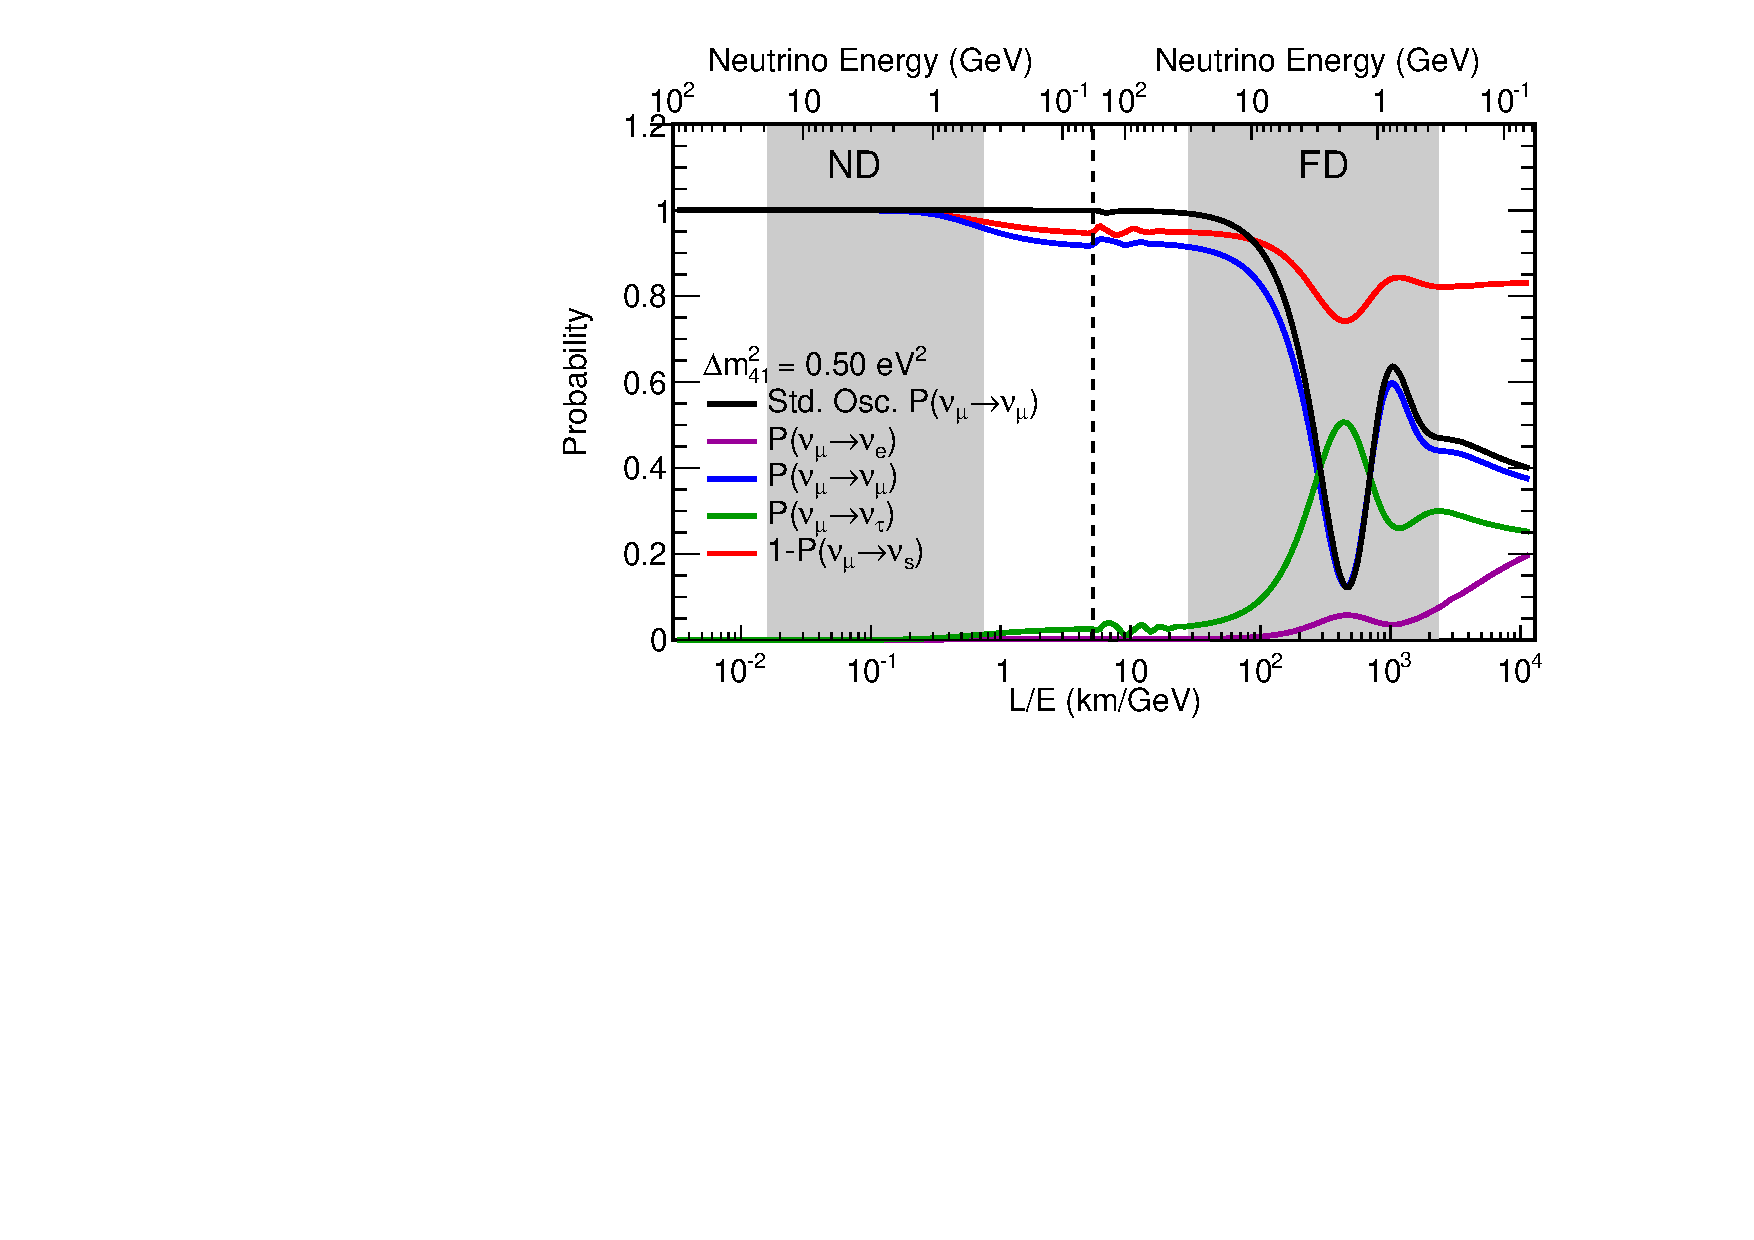
\includegraphics[width=0.49\textwidth]{graphics/DUNE_SterileSensi_dm0_5.pdf}
        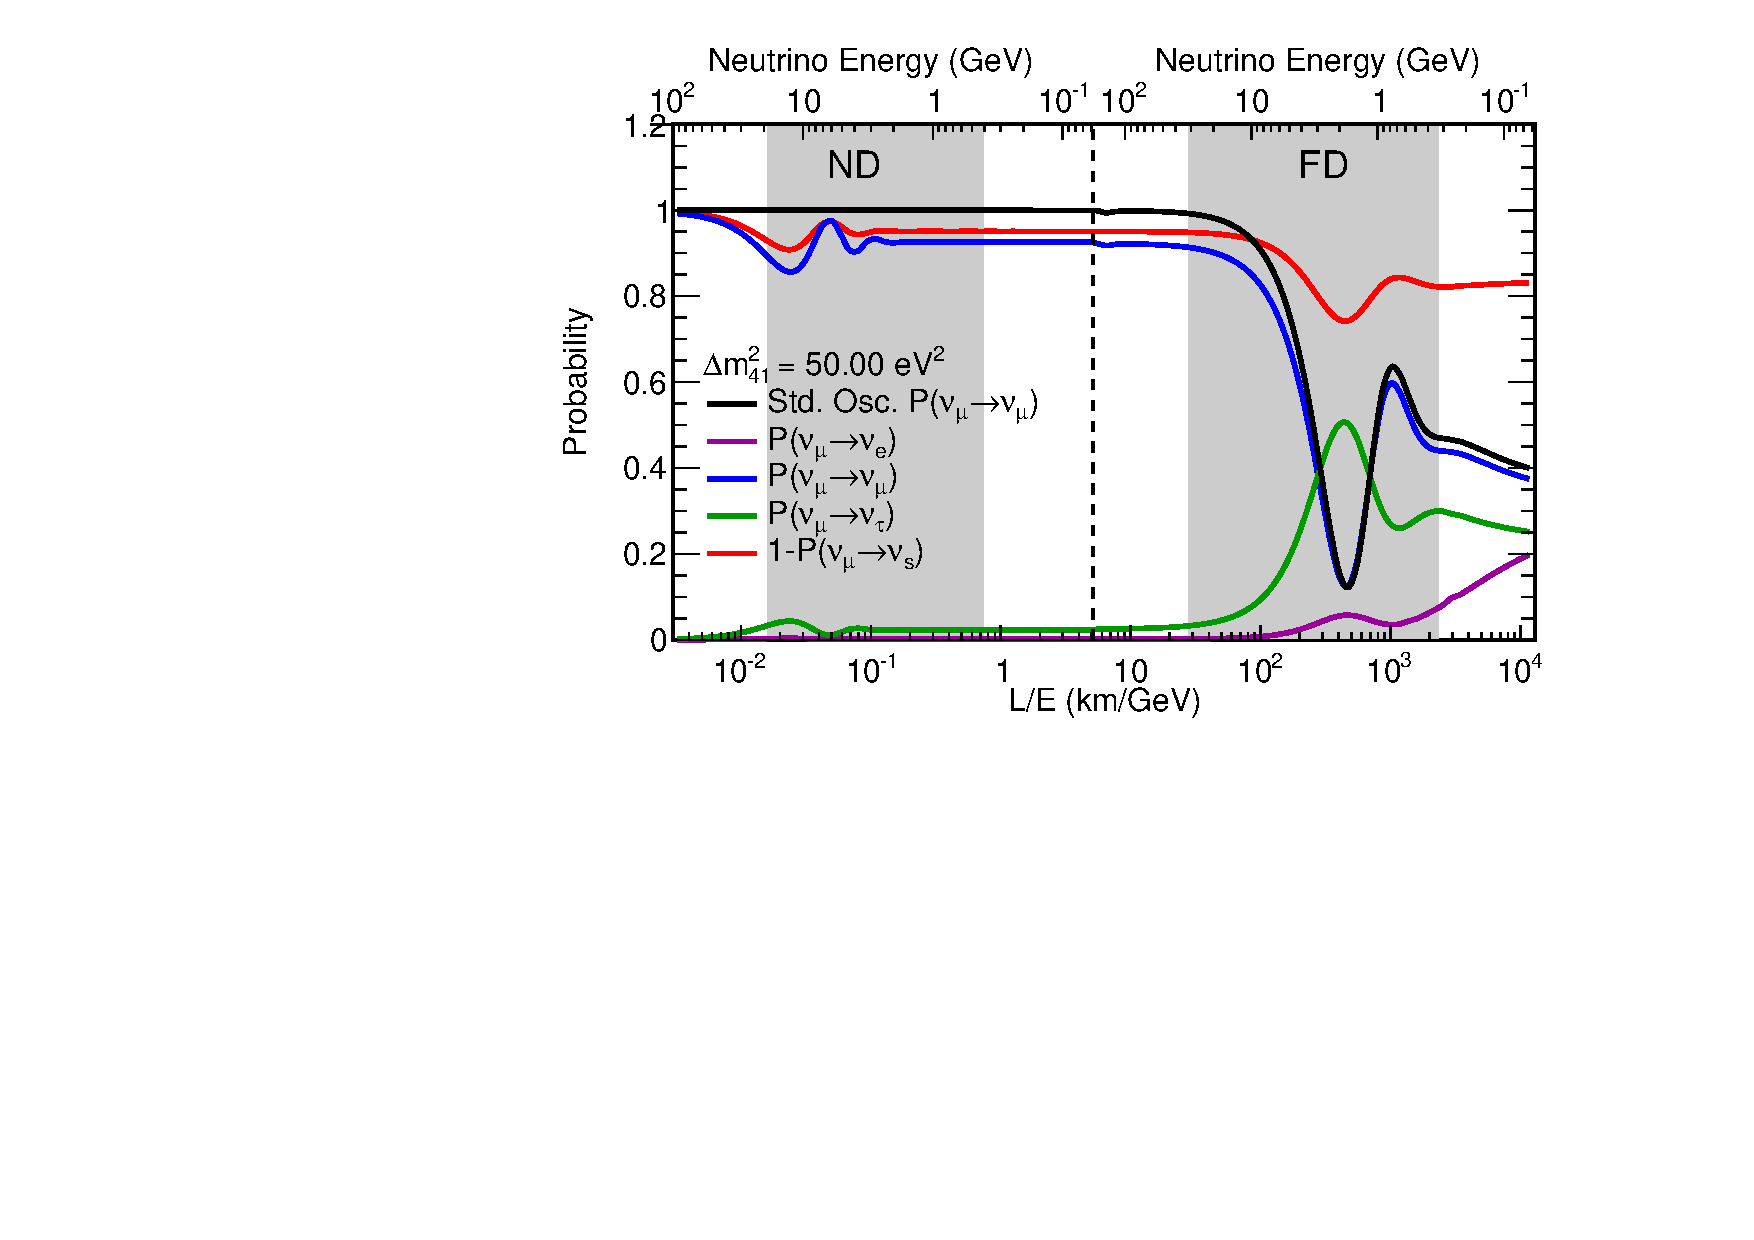
\includegraphics[width=0.49\textwidth]{graphics/DUNE_SterileSensi_dm50.pdf}
	\end{center}
\vspace{0pt}
\caption{Regions of $L/E$ probed by the DUNE detectors compared to 3-flavor and 3+1-flavor neutrino disappearance and appearance probabilities. The gray-shaded areas show the range of true neutrino energies probed by the Near (ND) and Far (FD) detectors. The top axis shows true neutrino energy, increasing from right to left. The top-left plot shows the probabilities assuming mixing with one sterile neutrino with $\Delta m^2_{\rm{41}}=0.05$~eV$^2$, corresponding to the Slow oscillations regime. The top-right plot assumes mixing with one sterile neutrino with $\Delta m^2_{\rm{41}}=0.5$~eV$^2$, corresponding to the Intermediate oscillations regime. The bottom plot includes mixing with one sterile neutrino with $\Delta m^2_{\rm{41}}=50$~eV$^2$, corresponding to the Rapid oscillations regime. As an example, the Slow sterile oscillations cause visible distortions in the three-flavor \numu~survival probability (blue curve) for neutrino energies $\sim10$\,GeV, well above the three-flavor oscillation minimum.}
  \label{fig:regimes}
 \vspace{0pt}
\end{figure}

\subsection{Setup and methods}
The simulation of the DUNE experimental setup was performed with the GLoBES software~\cite{Huber:2004ka,Huber:2007ji} using the DUNE CDR configuration presented in Ref.~\cite{Alion:2016uaj} as a starting point. The sterile neutrino effects have been implemented in GLoBES via the existing plug-in for sterile neutrinos and NSI~\cite{Joachim}. As described above, the Near detector will play a very important role in the sensitivity to sterile neutrinos both directly, for rapid oscillations with $\Delta m_{41}^2 > 1$~eV$^2$ where the sterile oscillation matches the Near detector baseline, and indirectly, at smaller values of $\Delta m_{41}^2$ where the Near detector is crucial to reduce the systematics affecting the Far detector to increase its sensitivity. To include these Near detector effects in these studies, the GLoBES DUNE CDR configuration was modified by adding a Near detector with correlated systematic errors with the Far detector. As a first approximation, the Near detector was assumed to be an identical scaled-down version of the Far detector where the same efficiencies, backgrounds and energy reconstruction from Ref.~\cite{Alion:2016uaj} have been assumed. Only the LArTPC portion of the detector is considered, and a mass of $83.76$~tons and a baseline of $0.575$~km are assumed. The systematic uncertainties defined in the GLoBES DUNE CDR configuration already take into account the effect of the Near detector reducing their impact. Thus, since we are now explicitly simulating the Near detector, larger uncertainties have been adopted but partially correlated between the different channels in the Near and Far detectorss, so that their impact is now reduced by the combination of both datasets. The full list of systematic uncertainties considered and their values is summarized in a technical note~\cite{ref:dune_steril_note}.

Finally, for oscillations observed at the Near detector, the uncertainty on the production point of the neutrinos can play an important role. We have included an additional $20\%$ energy smearing, which produces a similar effect given the $L/E$ dependence of oscillations. We implemented this smearing in the Near detector through multiplication of the migration matrices from Ref.~\cite{Alion:2016uaj} by an additional matrix with the $20\%$ energy smearing obtained by integrating the Gaussian
\begin{equation}
R^c(E,E')\equiv\frac{1}{\sigma(E)\sqrt{2\pi}}e^{-\frac{(E-E')^2}{2\sigma(E)}},
\label{R_mat}
\end{equation}
with $\sigma(E)=0.2 E$ in reconstructed energy $E'$.

\subsection{Results}
Studying the sensitivity to $\theta_{14}$, the dominant channels are those regarding $\nu_e$ disappearance. Therefore, only the $\nu_e$ CC sample is analyzed and the channels for NC and $\nu_{\mu}$ CC disappearance are not taken into account, as they do not influence greatly the sensitivity and they slow down the simulations. The sensitivity at $2\sigma$ level (2 d.o.f), taking into account the systematics mentioned above is shown in Figure~\ref{th_14}, along with a comparison to current constraints.
\begin{figure}
\centering
%$\vcenter{\hbox{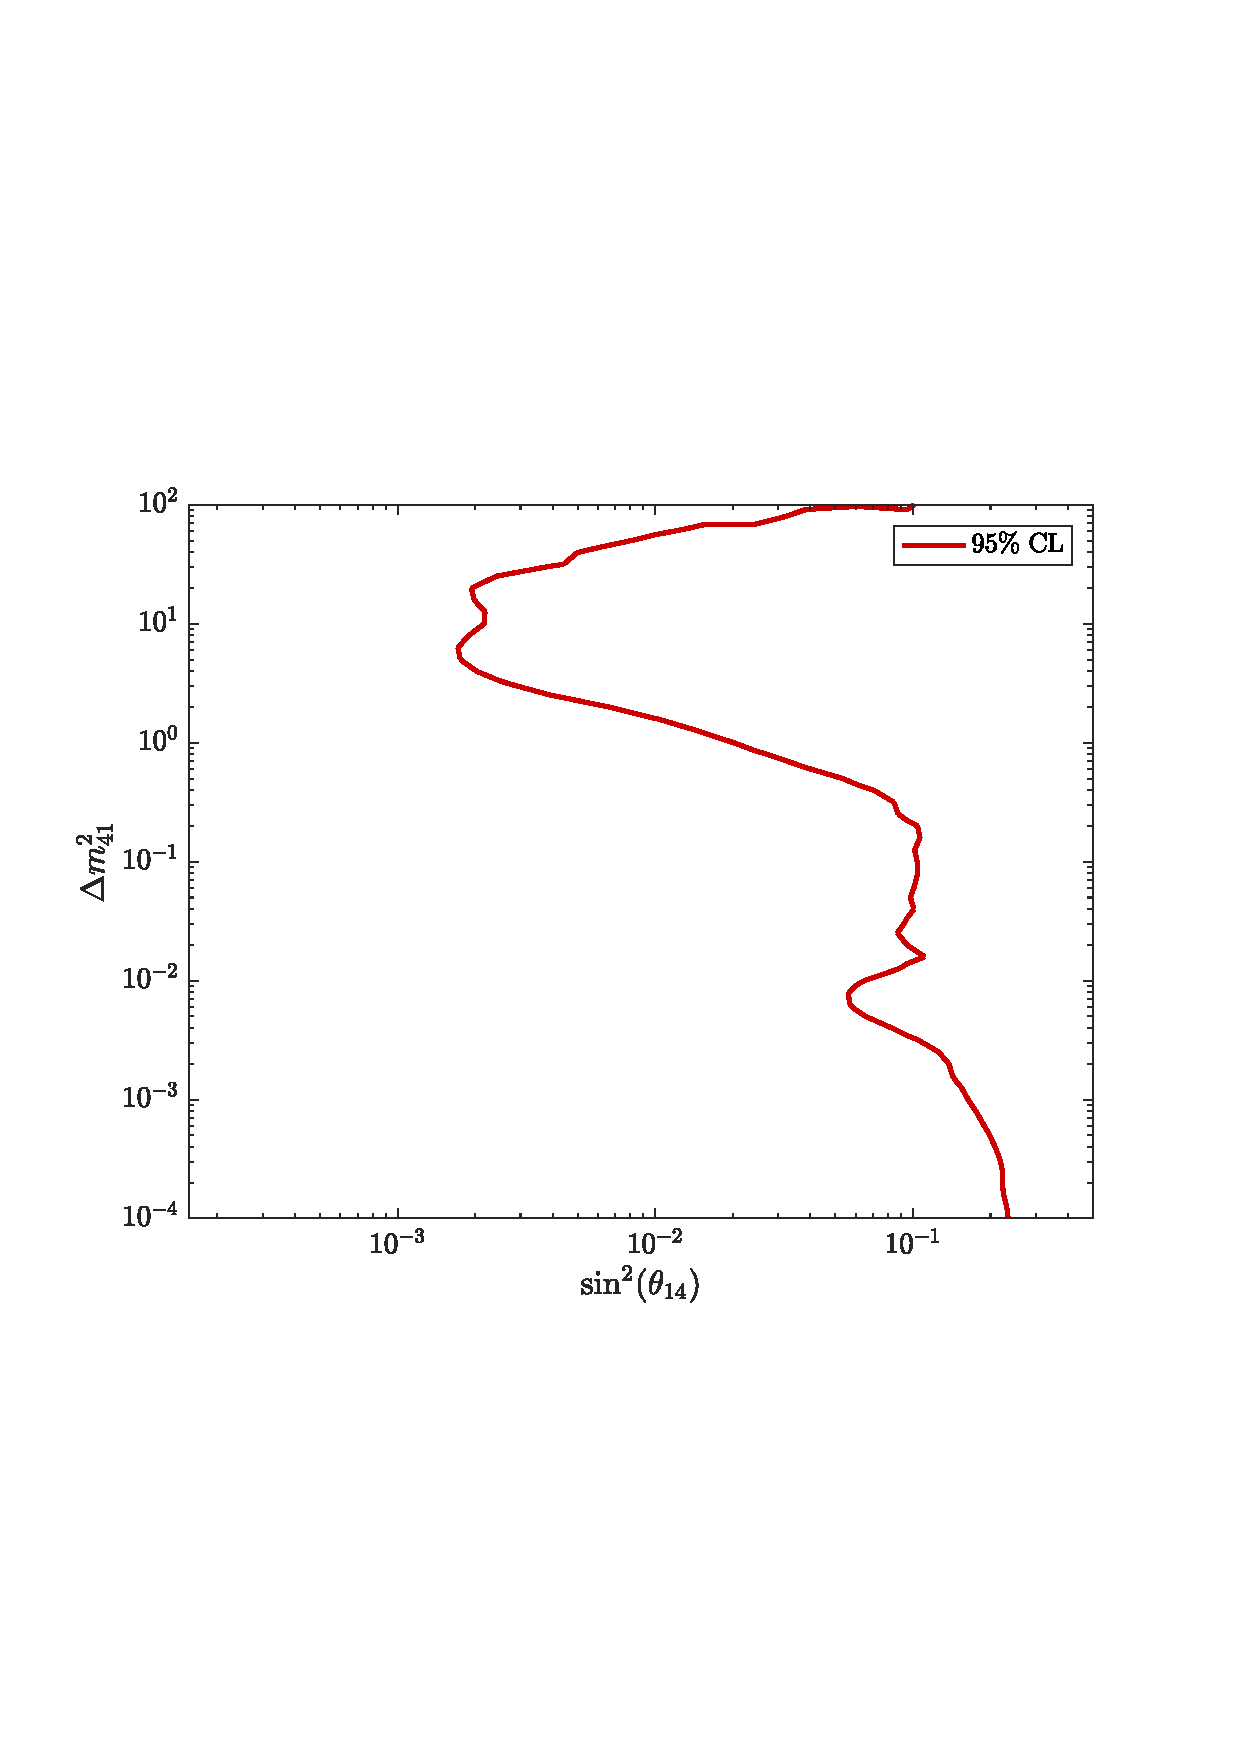
\includegraphics[width=0.45\columnwidth]{graphics/th_14_SMR_EOf}}}$
$\vcenter{\hbox{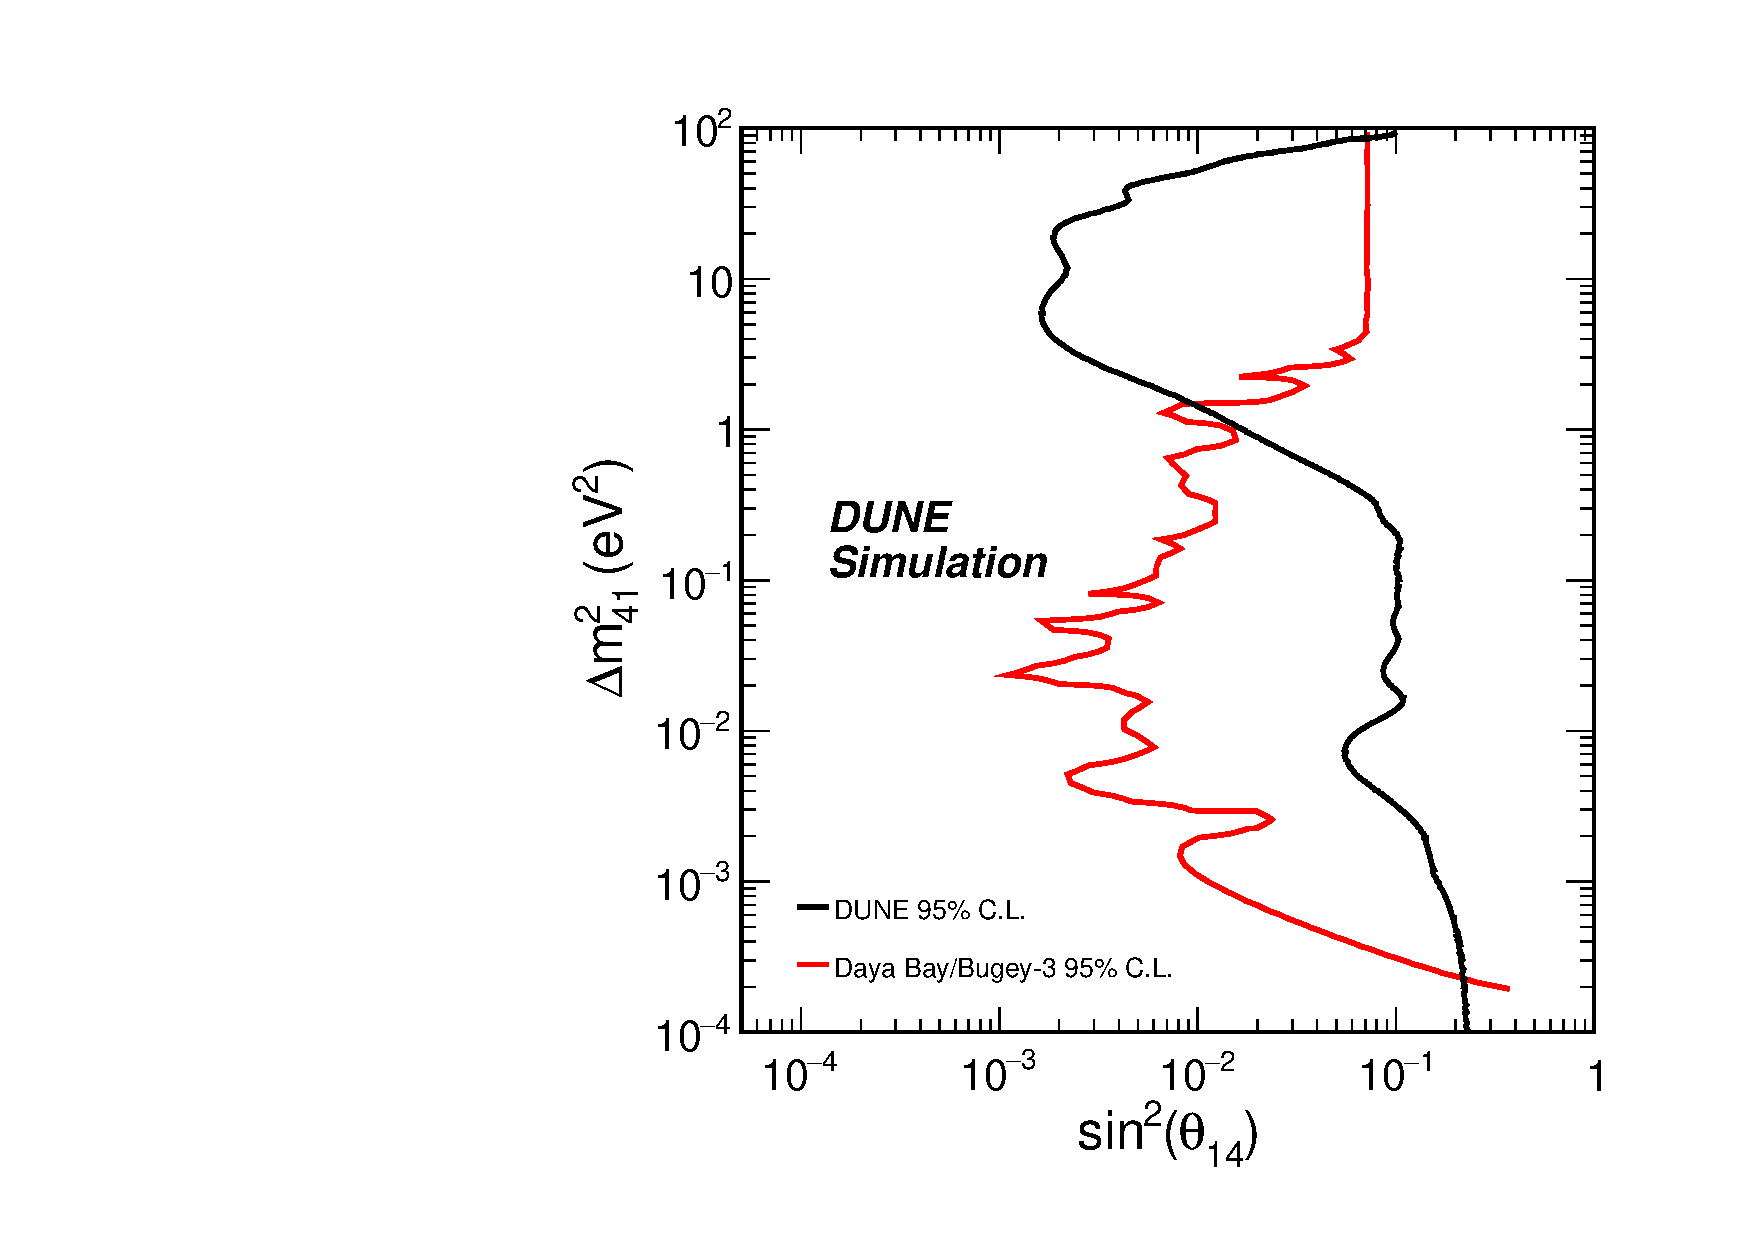
\includegraphics[width=0.45\columnwidth]{graphics/MultiPlots_DUNE_th14_prelim}}}$
%\setlength{\abovecaptionskip}{-40pt plus 1pt minus 1pt}
\caption{The DUNE sensitivity to $\theta_{14}$ from the $\nu_e$ CC samples at the Near and Far detectors is shown on the left-hand plot. Comparison with the combined reactor result from Daya Bay and Bugey-3 is shown on the right-hand plot. Regions to the right of the contour are excluded.}
\label{th_14}
\end{figure}

For the $\theta_{24}$ mixing angle, we analyze the $\nu_{\mu}$ CC disappearance, as well as the NC samples, which mainly contribute to the sensitivity. The results are shown in Fig.~\ref{th_24}, along with comparisons with present constraints.
\begin{figure}[!htbp]
\centering
%$\vcenter{\hbox{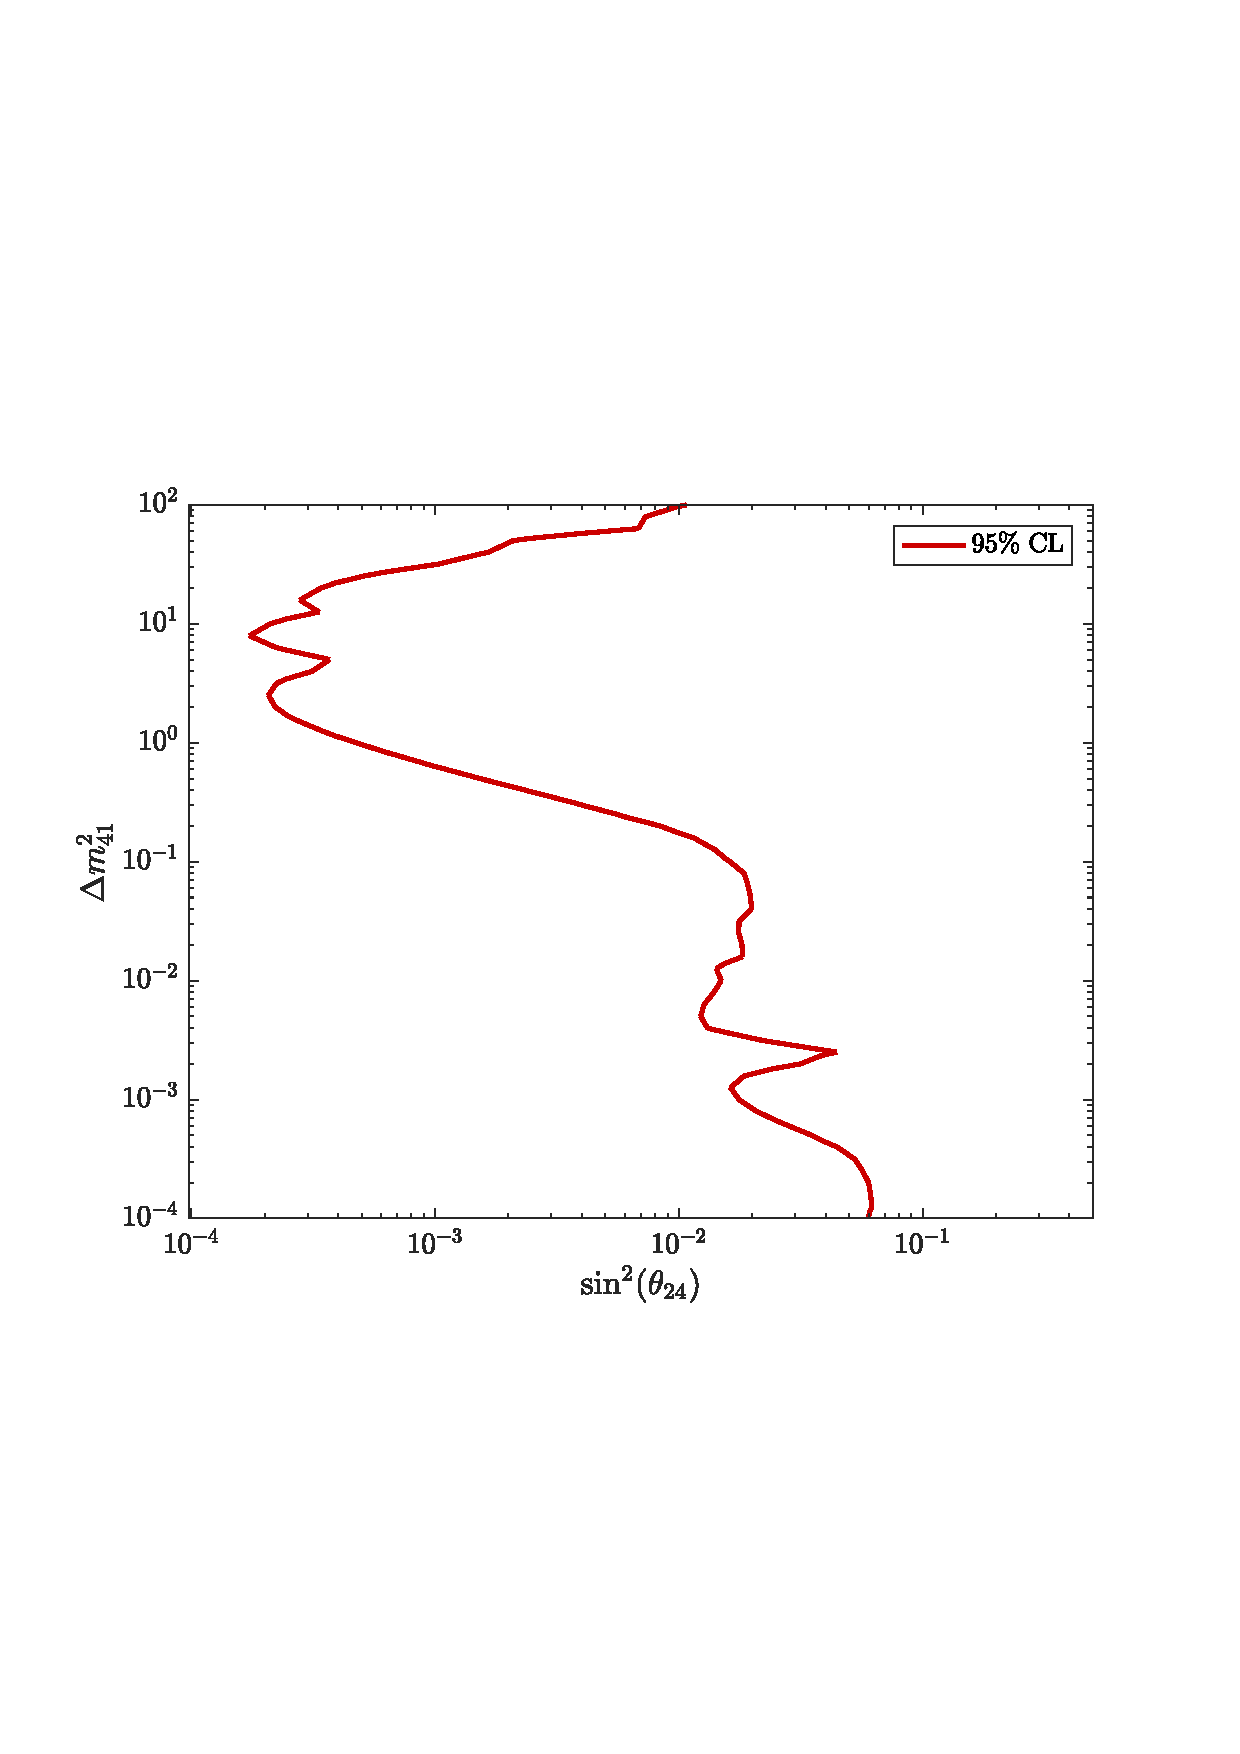
\includegraphics[width=0.45\columnwidth]{graphics/th_24_SMR_EOf}}}$
$\vcenter{\hbox{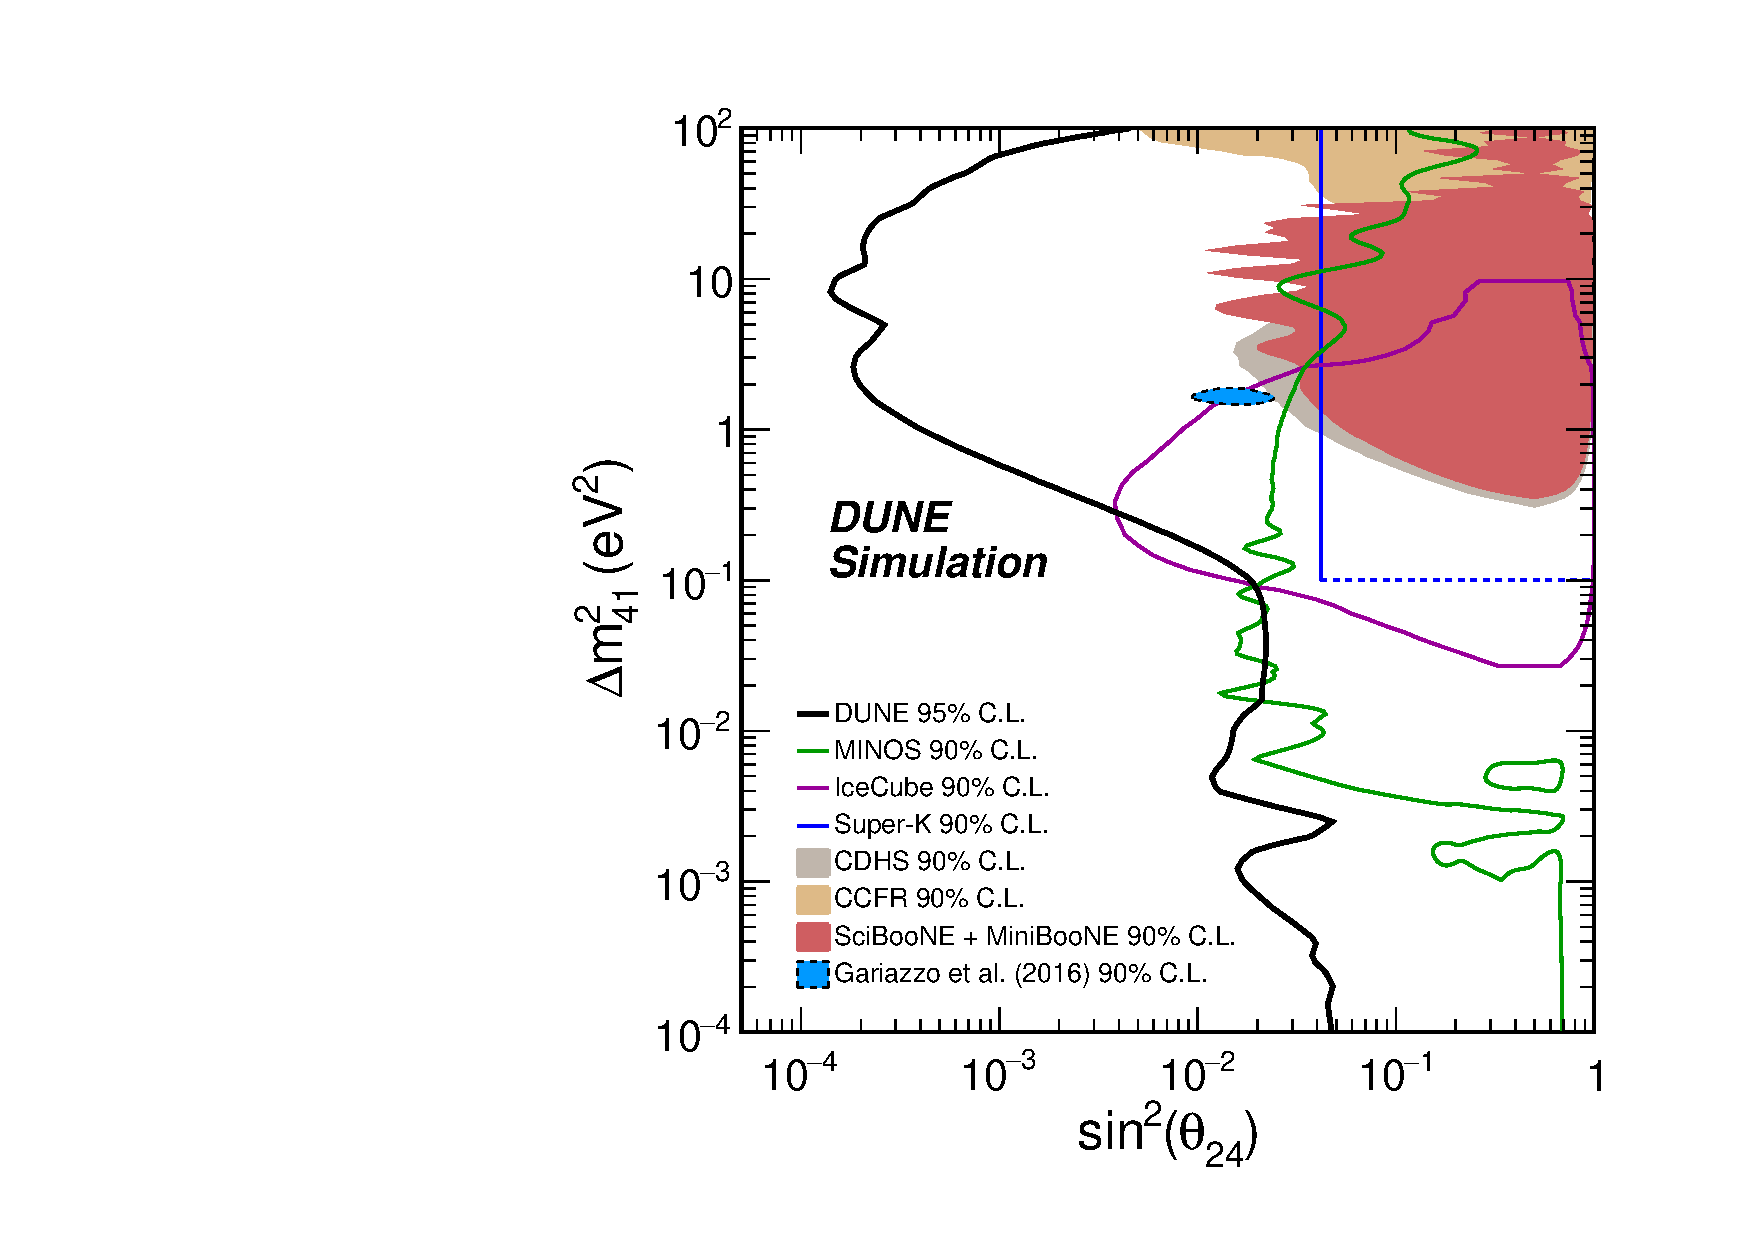
\includegraphics[width=0.45\columnwidth]{graphics/MultiPlots_DUNE_MINOS_IceCube_globAppF_prelim.pdf}}}$
%\setlength{\abovecaptionskip}{-40pt plus 1pt minus 1pt}
\caption{DUNE sensitivity to $\theta_{24}$ using the $\nu_\mu$ CC and NC samples at the Near and Far detectors is shown on the left-hand plot. A comparison with previous and existing experiments is shown on the right-hand plot. Regions to the right of the contour are excluded.}
\label{th_24}
\end{figure}
    In the case of the $\theta_{34}$ mixing angle, we analyze the NC sample, which exclusively contributes to the sensitivity. The results are shown in Fig.~\ref{th_34}. Further, a comparison with previous experiments sensitive to \numu, \nutau~mixing with large mass-squared splitting is possible by considering an effective mixing angle $\theta_{\mu\tau}$, such that $\sin^2{2\theta_{\mu\tau}}\equiv 4|U_{\tau4}|^2|U_{\mu 4}|^2=\cos^4\theta_{14}\sin^22\theta_{24}\sin^2\theta_{34}$, and assuming conservatively that $\cos^4\theta_{14}=1$, and $\sin^22\theta_{24}=1$. This comparison with previous experiments is also shown in Fig.~\ref{th_34}.
\begin{figure}
\centering
%$\vcenter{\hbox{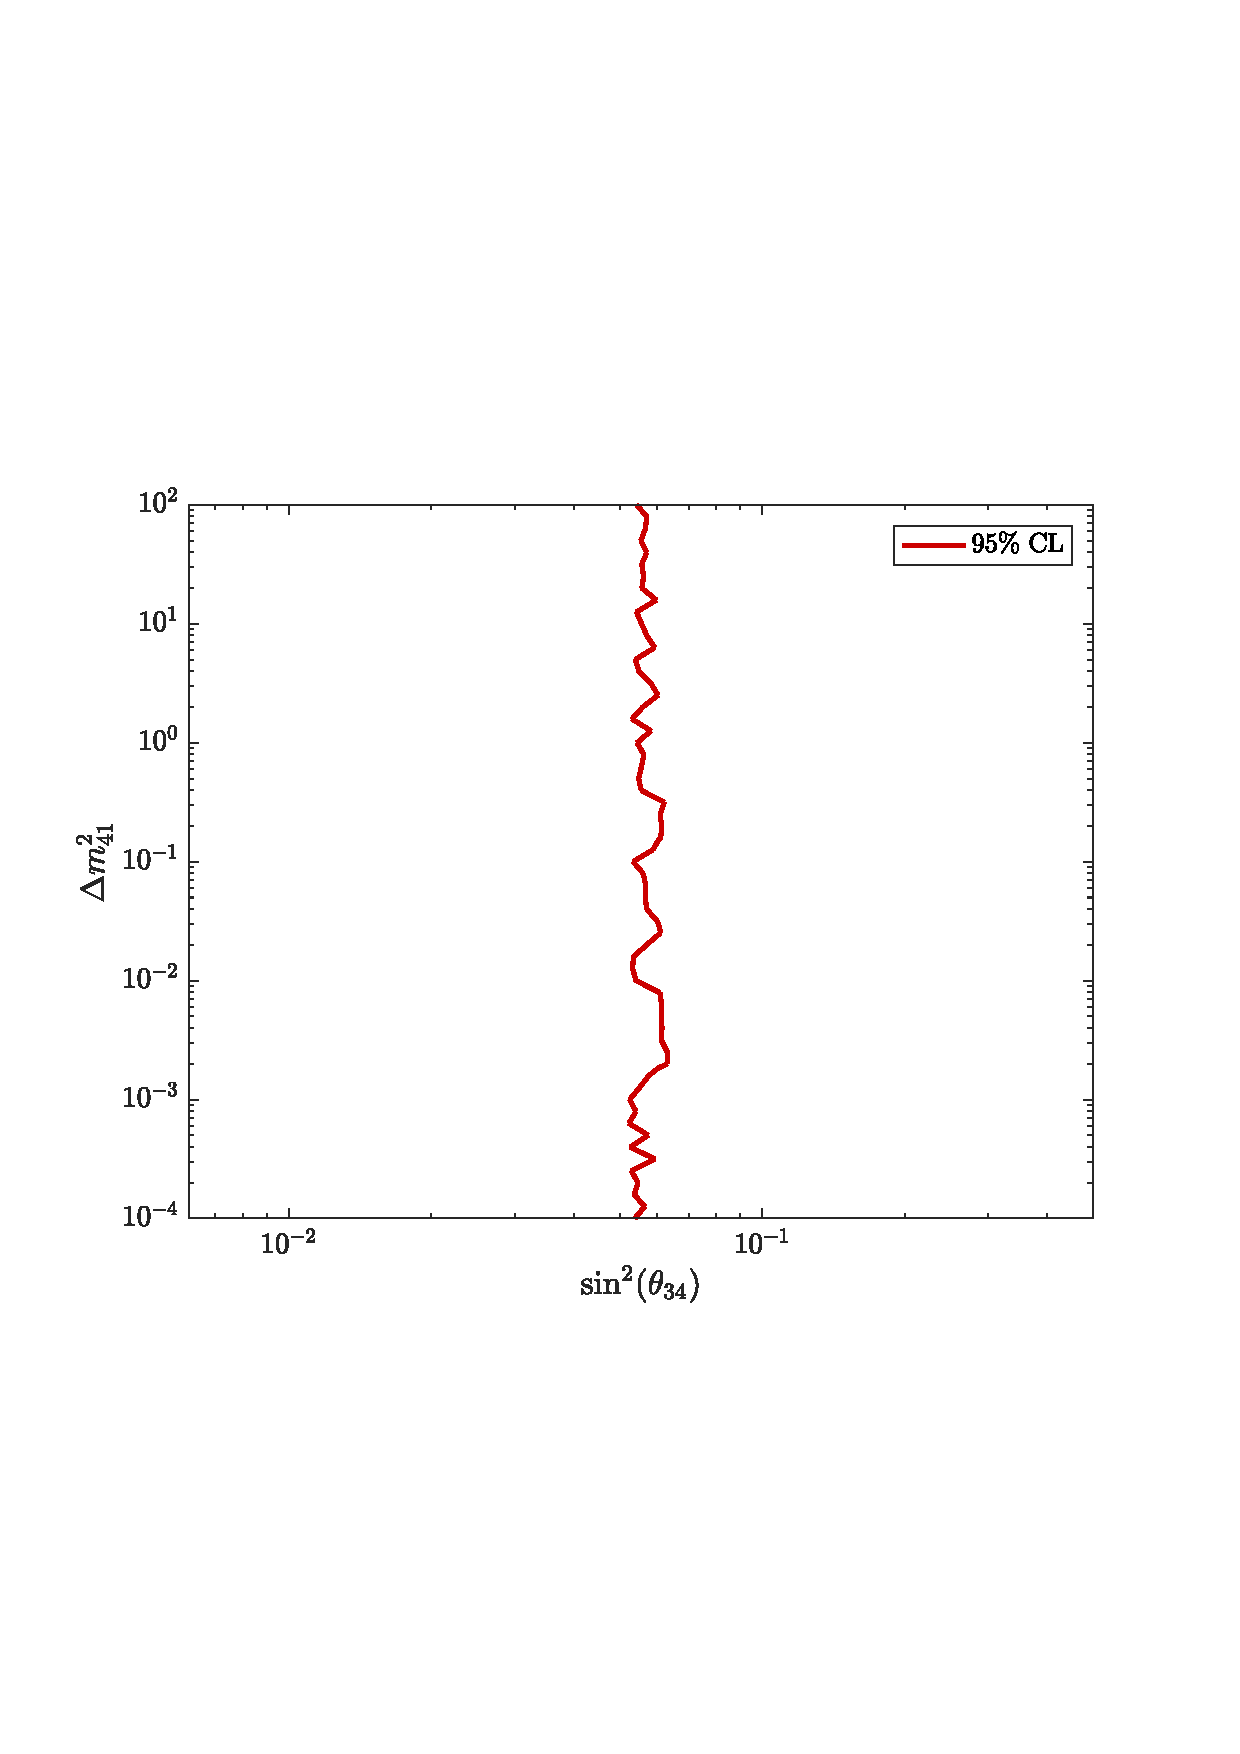
\includegraphics[width=0.45\columnwidth]{graphics/th_34_SMR_EOf}}}$
$\vcenter{\hbox{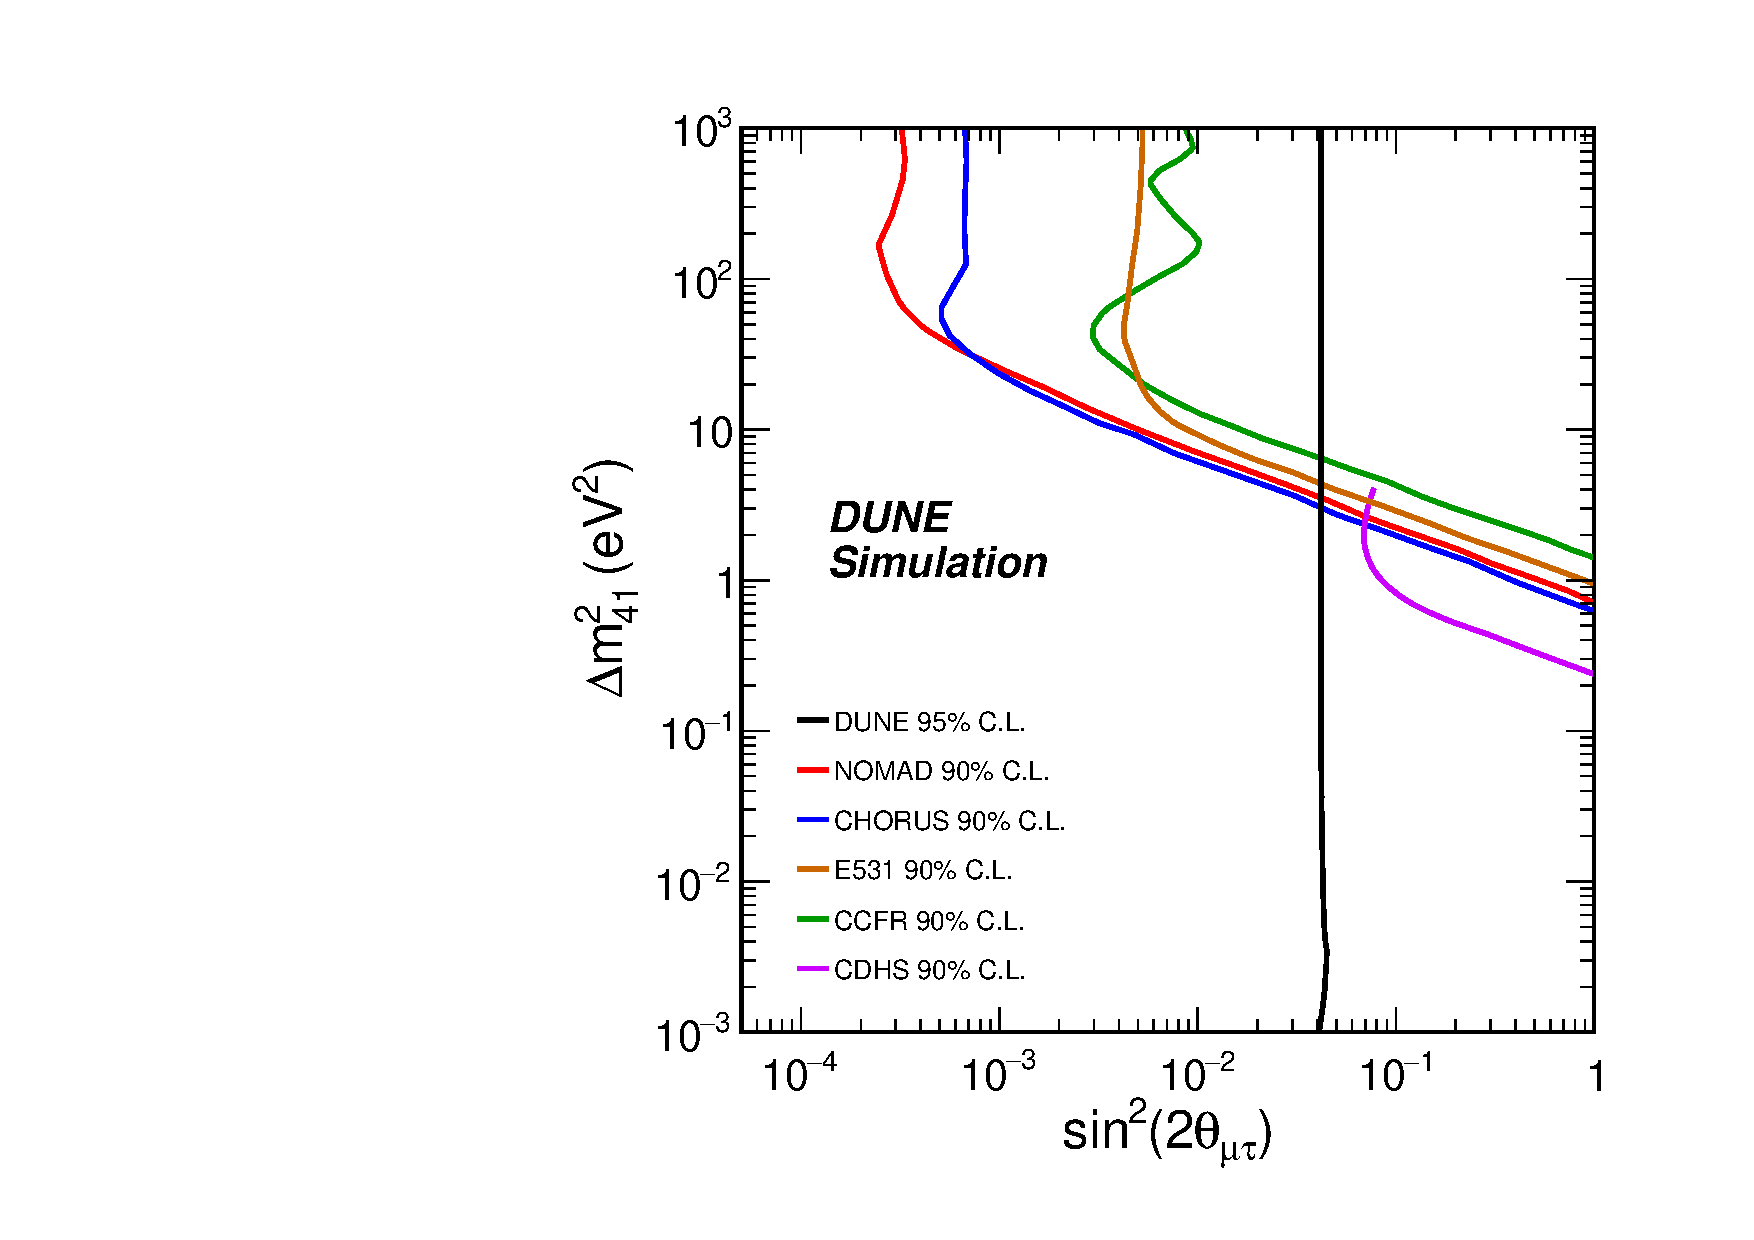
\includegraphics[width=0.45\columnwidth]{graphics/MultiPlots_DUNE_th34_prelim}}}$
%\setlength{\abovecaptionskip}{-40pt plus 1pt minus 1pt}
\caption{DUNE sensitivity to $\theta_{34}$ using the NC samples at the Near and Far detectors is shown on the left-hand plot. A comparison with previous and existing experiments is shown on the right-hand plot. Regions to the right of the contour are excluded.}
\label{th_34}
\end{figure}

Another quantitative comparison of our results for $\theta_{24}$ and $\theta_{34}$ with existing constraints can be made for projected upper limits on the sterile mixing angles assuming no evidence for sterile oscillations is found, and picking the value of  $\Delta m^2_{41} = 0.5$~eV$^2$ corresponding to the simpler counting experiment regime. For the 3+1 model, upper limits of $\theta_{24}$\,$<$\,$2.6^{\circ}$ and $\theta_{34}$\,$<$\,$14.2^{\circ}$ are obtained at the $2\sigma$ or 95\% C.L. from the presented DUNE sensitivities. If expressed in terms of the relevant matrix elements
\begin{align}
|U_{\mu4}|^2 =&\,\,\cos^2\theta_{14}\sin^2\theta_{24} \\
|U_{\tau4}|^2= & \,\,\cos^2\theta_{14}\cos^2\theta_{24}\sin^2\theta_{34},
\label{eq:DisapToApp}
\end{align}
these limits become $|U_{\mu4}|^{2}$\,$<$\,0.002 and $|U_{\tau4}|^{2}$\,$<$\,0.06 at the 95\% C.L., where we conservatively assume $\cos^2\theta_{14}$\,=\,1 in both cases, and additionally $\cos^2\theta_{24}$\,=\,1 in the second case.
\begin{table}[!ht]
  \centering
  \begin{tabular}{c c c c c }
    \hline\hline
    & $\theta_{24}$ & $\theta_{34}$ & $|U_{\mu4}|^2$ & $|U_{\tau4}|^2$  \\
    \hline
    DUNE  & $2.6^{\circ}$ & $14.2^{\circ}$ & 0.002 & 0.06  \\
    NOvA  & $20.8^{\circ}$ & $31.2^{\circ}$ & 0.126 & 0.268  \\
    %NOvA 2017  & $16.2^{\circ}$ & $29.8^{\circ}$ & 0.078 & 0.220 \\
    MINOS & $7.3^{\circ}$ & $26.6^{\circ}$ & 0.016 & 0.20  \\
    SuperK & $11.7^{\circ}$ & $25.1^{\circ}$ & 0.041 & 0.18  \\
    IceCube & $4.1^{\circ}$ & \-- & 0.005 & \--   \\
    IceCube-DeepCore & $19.4^{\circ}$ & $22.8^{\circ}$ & 0.11 & 0.15  \\
    \hline\hline
  \end{tabular}%
    \caption{The projected DUNE 95\% C.L. upper limits on sterile mixing angles and matrix elements compared to the equivalent 90\% C.L. upper limits from NOvA~\cite{ref:novasterile}, MINOS~\cite{ref:minossterile}, Super-Kamiokande~\cite{ref:superksterile}, IceCube~\cite{ref:IceCube}, and IceCube-DeepCore~\cite{ref:DeepCore}. The limits are shown for $\Delta m^2_{41} = 0.5$~eV$^2$ for all experiments, except for IceCube-DeepCore, where the results are reported for $\Delta m^2_{41} = 1.0$~eV$^2$.}
  \label{tab:limits}
\end{table}  
  
  
Finally, sensitivity to the $\theta_{\mu e}$ effective mixing angle, defined above as $\sin^2{2\theta_{\mu e}}\equiv 4|U_{e4}|^2|U_{\mu 4}|^2=\sin^22\theta_{14}\sin^2\theta_{24}$, is shown in Fig.~\ref{th_me}, which also displays a comparison with the allowed regions from LSND and MiniBooNE, as well as with present constraints and projected constraints from the Fermilab Short-Baseline Neutrino (SBN) program.
\begin{figure}[!htbp]
\centering
%$\vcenter{\hbox{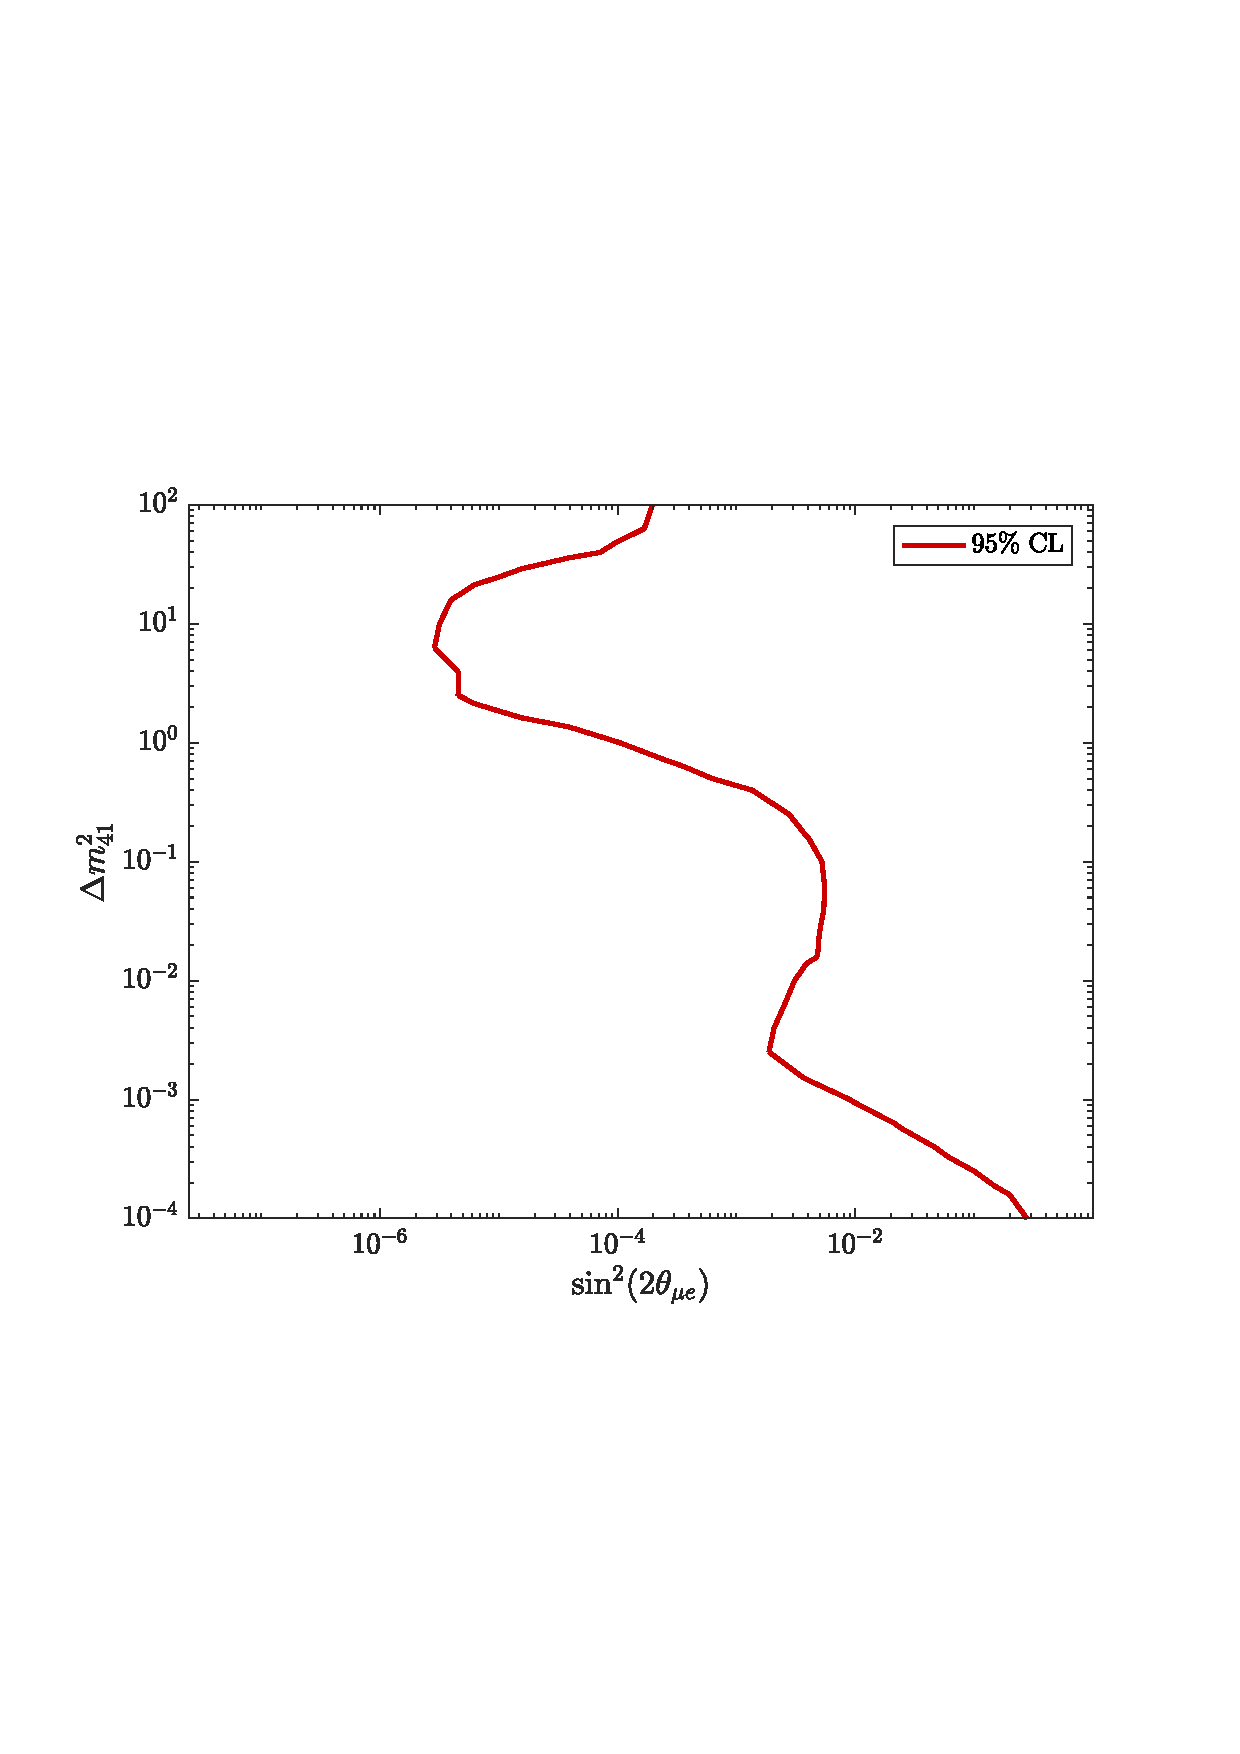
\includegraphics[width=0.45\columnwidth]{graphics/th_me_SMR_EOf}}}$
$\vcenter{\hbox{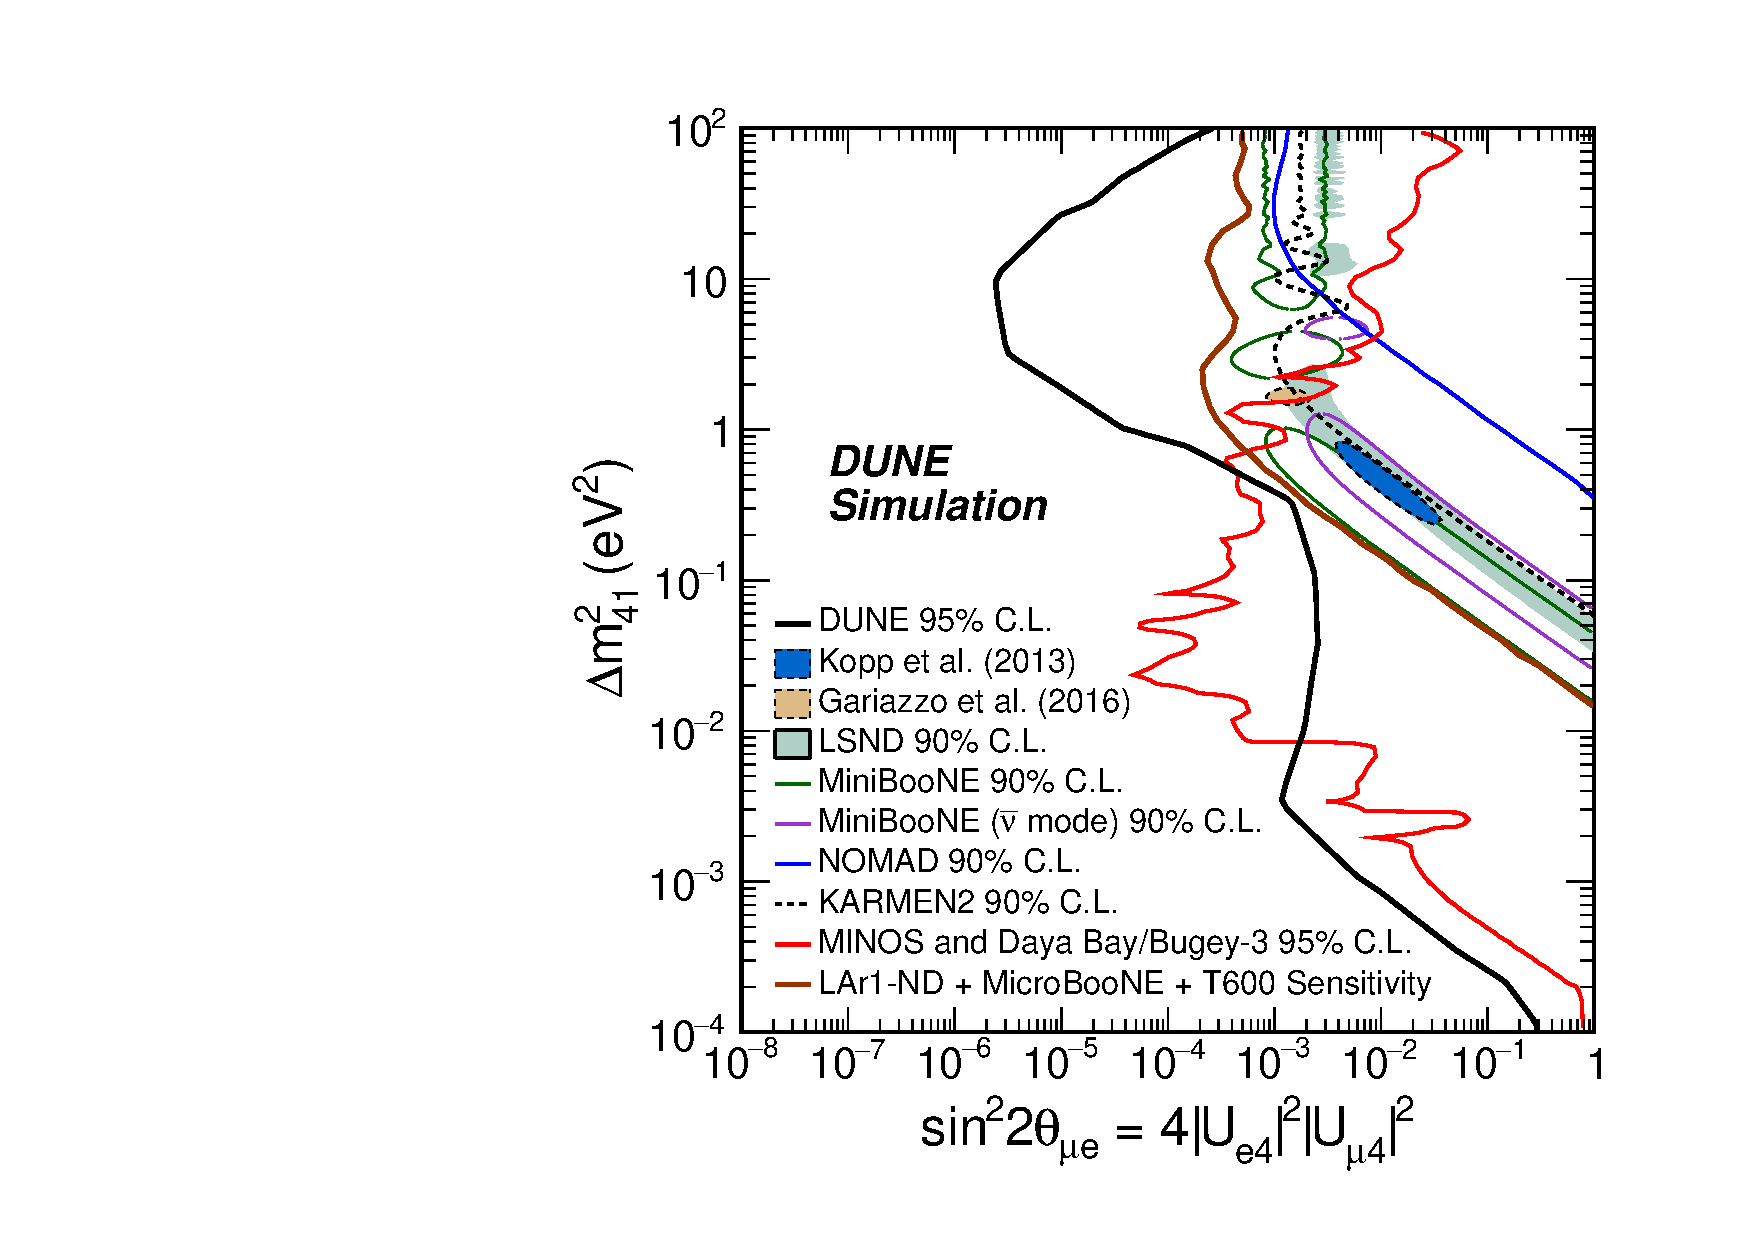
\includegraphics[width=0.45\columnwidth]{graphics/ComboLimit95_dune_sbn.pdf}}}$
%\setlength{\abovecaptionskip}{-40pt plus 1pt minus 1pt}
\caption{DUNE sensitivity to $\theta_{\mu e}$ from the appearance and disappearance samples at the Near and Far detectors is shown on the left-hand plot. A comparison with previous existing experiments and the sensitivity from the future Short-Baseline Neutrino program is shown on the right-hand plot. Regions to the right of the contour are excluded.}
\label{th_me}
\end{figure}

To illustrate that DUNE would not be limited to constraining regions of parameter space describing active-sterile neutrino mixing, we have produced a discovery potential plot, for a scenario with one sterile neutrino governed by the LSND best-fit parameters $\left(\Delta m_{14}^2= 1.2\;\text{eV}^2;\,\,\sin^2{2\theta_{\mu e}}=0.003\right)$~\cite{LSNDSterile}. A small $2\sigma$ allowed region, shown in Fig.~\ref{Dis_plot_me}, is obtained, which can be compared with the LSND allowed region in Fig.~\ref{th_me}. 
\begin{figure}[!h]
\centering
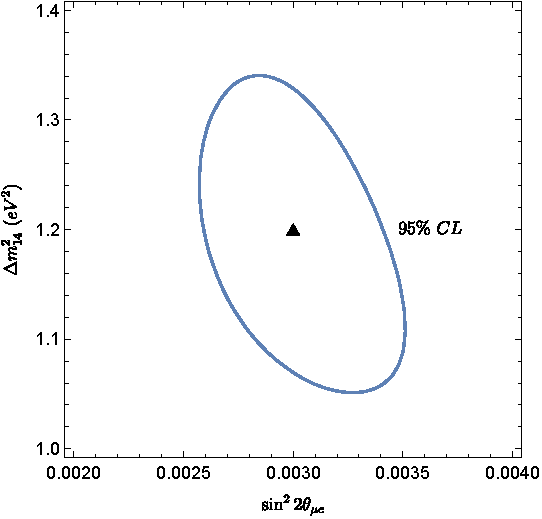
\includegraphics[scale=0.8]{graphics/dpme}
\caption{Discovery plot assuming $\theta_{\mu e}$ and $\Delta m_{41}^2$ are at the LSND anomaly best-fit point~\cite{LSNDSterile}.}
\label{Dis_plot_me}
\end{figure}

The physics reach plots shown above illustrate the excellent potential of DUNE to discover or constrain mixing with sterile neutrinos. Notably, in the case of sterile-mediated \numu~to \nue~transistions, DUNE can place very competitive constraints on its own, without requiring a combination with reactor experiments. 

\subsection{Discussion of potential enhancements from hardware improvements}
These studies show compelling motivation for DUNE to deploy a highly-capable Near detector given its high potential for discovery or constraining of new physics, including mixing with sterile neutrino species.



%%%%%%%%%%%%%%%%%%%%%%%%%%%%%%%%%%%%%%%%%%%%%%%%%%%%%%%%%%%%
%%% NEUTRINO TRIDENTS %%%%%%%%%%%%%%%%%%%%%%%%%%%%%%%%%%%%%%
\section{Search for Neutrino tridents at the Near Detector}
%%%%%%%%%%
Neutrino trident production is a weak process in which a neutrino, scattering off the Coulomb field of a heavy nucleus, generates a pair of charged leptons ~\cite{Czyz:1964zz,Lovseth:1971vv,Fujikawa:1971nx,Koike:1971tu,Koike:1971vg,Brown:1973ih,Belusevic:1987cw}. Measurements of muonic neutrino tridents ($\nu_\mu \to \nu_\mu \mu^+\mu^-$) were carried out at the CHARM-II~\cite{Geiregat:1990gz}, CCFR~\cite{Mishra:1991bv} and NuTeV~\cite{Adams:1999mn} experiments:
%%%%%%%%%%
\[
\frac{\sigma(\nu_\mu \to \nu_\mu \mu^+\mu^-)_\text{exp}}{\sigma(\nu_\mu \to \nu_\mu \mu^+\mu^-)_\text{SM}} = 
\begin{cases}
1.58 \pm 0.64         & \text{(CHARM-II)} \\ 
0.82 \pm 0.28         & \text{(CCFR)} \\
0.72 ^{+1.73}_{-0.72} & \text{(NuTeV)} 
\end{cases}
\]
%%%%%%%%%%
The high-intensity muon-neutrino beam at the DUNE near detector will lead to a sizable production rate of trident events (see Table~\ref{tab:trident_rates}), offering excellent prospects to improve the above measurements. A deviation from the event rate predicted by the SM could be an indication of new interactions mediated by the corresponding new gauge bosons~\cite{Altmannshofer:2014pba}. 

%%%%%%%%%%%%%%%%%%%%%%%%%%%%%%
\begin{table}[!b]
\begin{center}
\begin{tabular}{lcccc}
\toprule
& \multicolumn{2}{c}{Reference beam, 80~GeV} & \multicolumn{2}{c}{Optimized beam, 120~GeV} \\
& coherent & incoherent & coherent & incoherent \\
\midrule
$\nu_\mu \to \nu_\mu \mu^+\mu^-$ & $2.05 \pm 0.12$ & $0.87 \pm 0.27$ & $1.17 \pm 0.07$ & $0.49 \pm 0.15$ \\
$\nu_\mu \to \nu_\mu e^+e^-$ & $4.92 \pm 0.29$ & $0.32 \pm 0.10$ & $2.84 \pm 0.17$ & $0.18 \pm 0.06$\\
$\nu_\mu \to \nu_e e^+\mu^-$ & $17.4 \pm 1.0$ & $2.2 \pm 0.7$ & $9.8 \pm 0.6$ & $1.2 \pm 0.4$ \\
$\nu_\mu \to \nu_e \mu^+e^-$ & $0$ & $0$ & $0$ & $0$ \\
\midrule
$\bar\nu_\mu \to \bar\nu_\mu \mu^+\mu^-$ & $1.54 \pm 0.09$ & $0.67 \pm 0.21$ & $0.72 \pm 0.04$ & $0.32 \pm 0.10$ \\
$\bar\nu_\mu \to \bar\nu_\mu e^+e^-$ & $4.03 \pm 0.24$ & $0.26 \pm 0.08$ & $2.21 \pm 0.13$ & $0.13 \pm 0.04$ \\
$\bar\nu_\mu \to \bar\nu_e e^+\mu^-$ & $0$ & $0$ & $0$ & $0$ \\
$\bar\nu_\mu \to \bar\nu_e \mu^+e^-$ & $13.8 \pm 0.8$ & $1.7 \pm 0.5$ & $7.0 \pm 0.4$ & $0.9 \pm 0.3$ \\
\bottomrule
\end{tabular}
\end{center}
\caption{Expected number of Standard Model $\nu_\mu$ and $\bar\nu_\mu$-induced trident events at the DUNE near detector per tonne of argon and year of operation, and for two neutrino beam configurations, the 80~GeV reference beam from the DUNE CDR~\cite{cdr-vol-2} and the engineered optimized 120~GeV beam from~\cite{fields_doc_2901}. We assume $1.47 \times 10^{21}$~POT per year for the 80~GeV beam~\cite{cdr-vol-2} and  $1.1 \times 10^{21}$~POT per year for the 120~GeV beam~\cite{fields_doc_2901}.}
\label{tab:trident_rates}
\end{table}
%%%%%%%%%%%%%%%%%%%%%%%%%%%%%%

The main challenge in obtaining a precise measurement of the muonic trident cross section will be the copious backgrounds, mainly consisting of charged-current single-pion production events, $\nu_\mu N \to \mu \pi N^\prime$, as muon and pion tracks can be easily confused in LArTPC detectors. The discrimination power of the DUNE-ND LArTPC was evaluated using large simulation datasets of signal and background. Each simulation event represents a different neutrino-argon interaction in the active volume of the detector. Signal events were generated using a standalone code \cite{} that simulates trident production of muons and electrons through the scattering of $\nu_mu$ and $\nu_e$ on argon or iron nuclei. The generator considers both the coherent scattering on the full nucleus (the dominant contribution) and the incoherent scattering on individual nucleons. Background events, consisting of several SM neutrino interactions, were generated using GENIE. Roughly $30\%$ of the generated events have a charged pion in the final state, leading to two charged tracks with muon-like energy deposition pattern ($\mathrm{d}E/\mathrm{d}x$), as in our trident signal. All final-state particles produced in the interactions were propagated through the detector geometry using the Geant4-based \cite{Agostinelli:2002hh,Allison:2006ve,Allison:2016lfl} simulation of the DUNE ND. Charge collection and readout were not simulated, and possible inefficiencies due to mis-reconstruction effects or event pile-up were disregarded for simplicity.

%%%%%%%%%%%%%%%%%%%%%%%%%%%%%%
\begin{figure}[!tb]
\centering
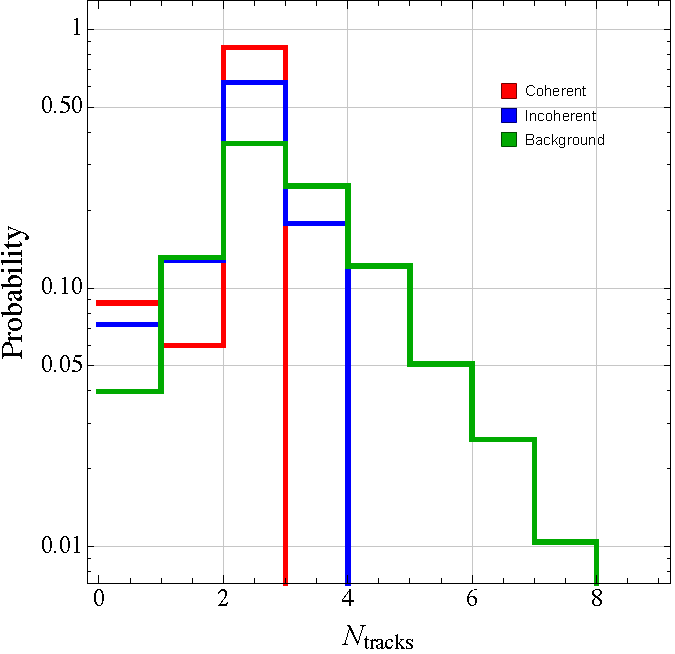
\includegraphics[height=5cm]{graphics/NTracksHistogram.pdf}
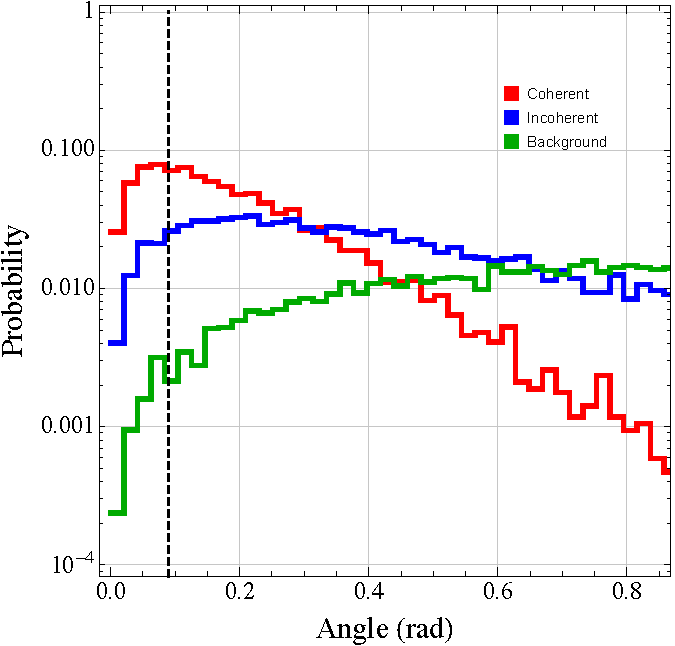
\includegraphics[height=5cm]{graphics/AngleHistogram.pdf} \\[0.75\baselineskip]
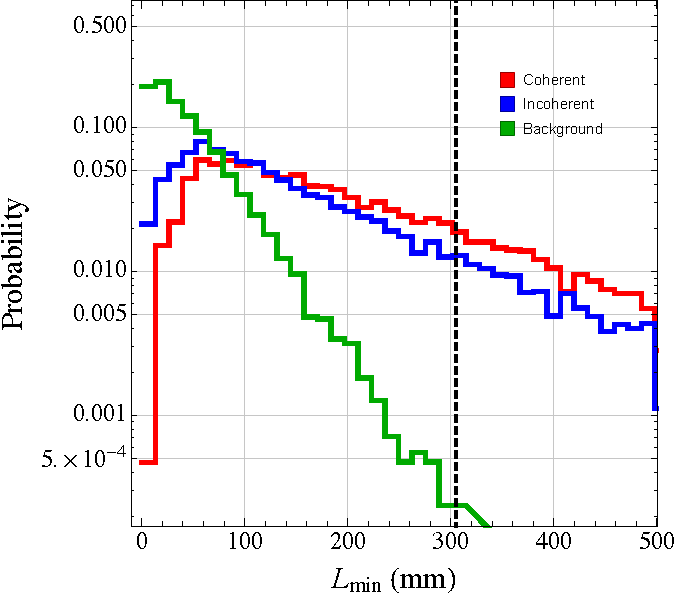
\includegraphics[height=5cm]{graphics/LengthHistogram.pdf}
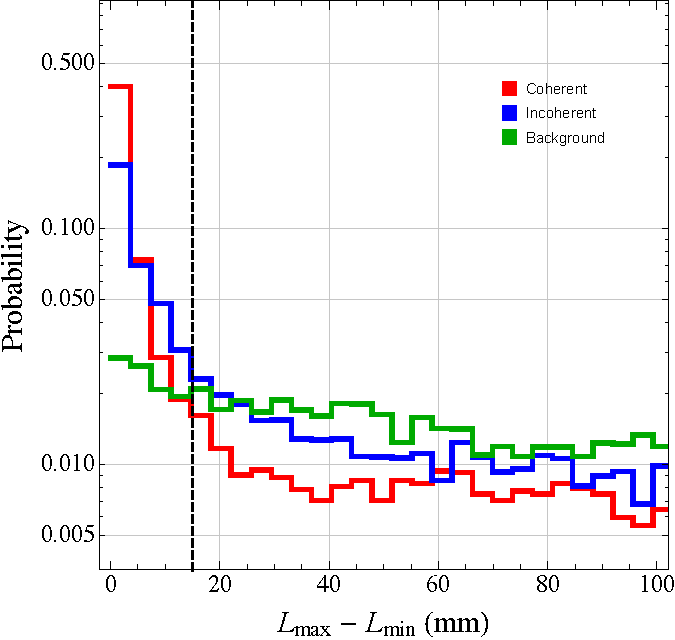
\includegraphics[height=5cm]{graphics/DeltaLHistogram.pdf}
\caption{Event kinematic distributions of signal and background considered for the selection of muonic trident interactions in the ND LArTPC: number of tracks (top left), angle between the two main tracks (top right), length of the shortest track (bottom left), and the difference in length between the two main tracks (bottom right). The dashed, black vertical lines indicate the optimal cut values used in the analysis.} \label{fig:trident_kinematics}
\end{figure}
%%%%%%%%%%%%%%%%%%%%%%%%%%%%%%

Figure~\ref{fig:trident_kinematics} shows the distribution (area normalized) for signal and background of the different kinematic variables used in our analysis for the discrimination between signal and background. As expected, background events tends to contain a higher number of tracks than the signal. The other distributions also show a clear discriminating power: the angle between the two tracks is typically much smaller in the signal, than in the background. Moreover, the signal tracks (two muons) tend to be longer than tracks in the background (mainly one muon plus one pion).

%%%%%%%%%%%%%%%%%%%%%%%%%%%%%%%%%%%%%%%%%%%%%%%%%%%%%%%%%%%%
\subsection{Sensitivity to new physics}
%%%%%%%%%%
The sensitivity of neutrino tridents to heavy new physics (i.e.\ heavy compared to the momentum transfer in the process) can be parametrized in a model independent way using a modification of the effective four-fermion interaction Hamiltonian. Focusing on the case of muon-neutrinos interacting with muons, the vector and axial-vector couplings can be written as
%%%%%%%%%%
\begin{equation}
g_{\mu\mu\mu\mu}^V = 1 + 4 \sin^2\theta_W + \Delta g_{\mu\mu\mu\mu}^V \quad \mathrm{and} \quad g_{\mu\mu\mu\mu}^A = -1 + \Delta g_{\mu\mu\mu\mu}^A ~,
\end{equation}
%%%%%%%%%%
where $\Delta g_{\mu\mu\mu\mu}^V$ and $\Delta g_{\mu\mu\mu\mu}^A$ parameterize possible new physics contributions. Couplings involving other combinations of lepton flavors can be modified analogously. Note, however, that for interactions that involve electrons, very strong constraints can be derived from LEP bounds on electron contact interactions~\cite{Schael:2013ita}. The modified interactions of the muon-neutrinos with muons alter the cross section of the $\nu_\mu N \to \nu_\mu \mu^+\mu^- N$ trident process. In Fig.~\ref{fig:trident_gVgA} we show the regions in the $\Delta g^V_{\mu\mu\mu\mu}$ vs.\ $\Delta g^A_{\mu\mu\mu\mu}$ plane that are excluded by the existing CCFR measurement $\sigma_\text{CCFR} / \sigma_\text{CCFR}^\text{SM} = 0.82 \pm 0.28$~\cite{Mishra:1991bv} at the 95\% C.L. in gray. A measurement of the $\nu_\mu N \to \nu_\mu \mu^+\mu^- N$ cross section with $25\%$ uncertainty at the DUNE near detector could cover the blue hashed regions. We see that the DUNE measurement could extend the coverage of new physics parameter space substantially.

%%%%%%%%%%%%%%%%%%%%%%%%%%%%%%%%%%%%%%%%%%%%%%%%%%%%%%%%%%%%%%%
\begin{figure}[tb!]
\centering
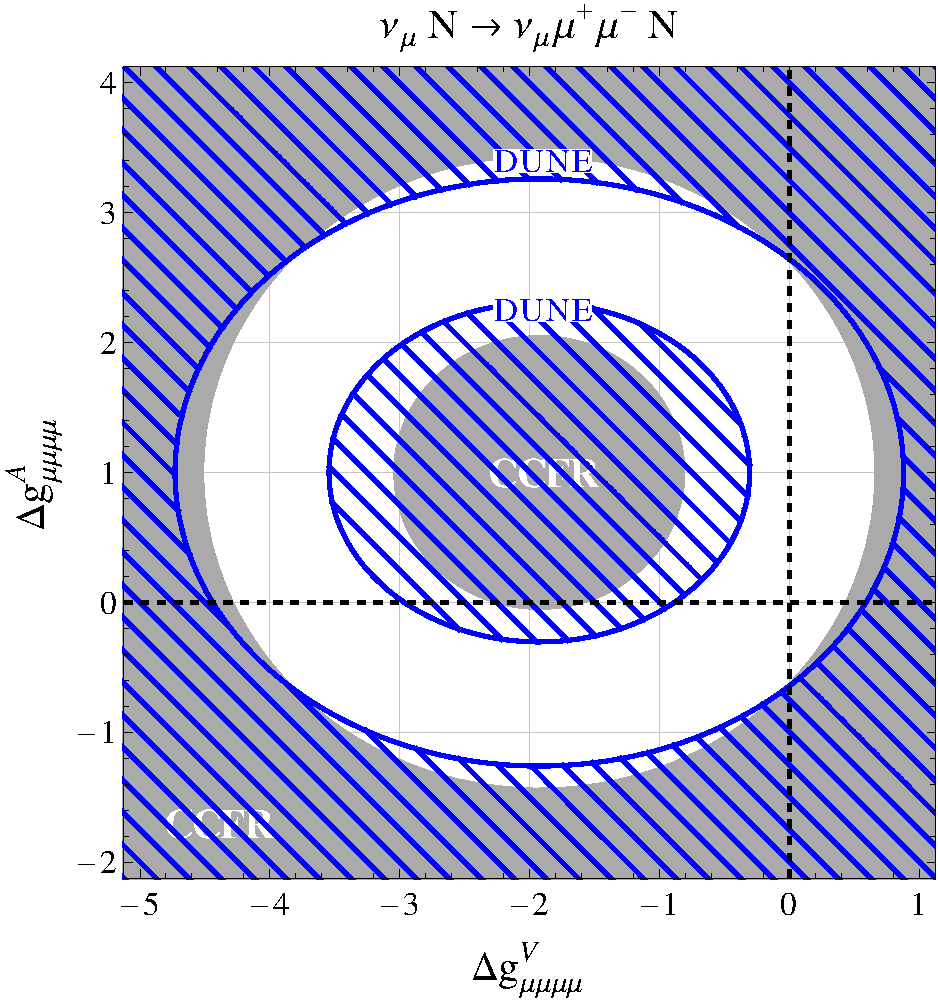
\includegraphics[width=0.5\textwidth]{graphics/model_independent.pdf}
\caption{Projected sensitivity (95\% CL) of a measurement of the $\nu_\mu N \to \nu_\mu \mu^+\mu^- N$ cross section at the DUNE near detector to modifications of the vector and axial-vector couplings of muon-neutrinos to muons (blue hashed regions). The gray regions are excluded at 95\% C.L. by existing measurements of the cross section by the CCFR collaboration. The intersection of the dashed lines indicates the SM point.}
\label{fig:trident_gVgA}
\end{figure}
%%%%%%%%%%%%%%%%%%%%%%%%%%%%%%%%%%%%%%%%%%%%%%%%%%%%%%%%%%%%%%%

A class of models that modify the trident cross section are those that contain an additional neutral gauge boson, $Z'$, that couples to neutrinos and charged leptons. A consistent way of introducing such a $Z'$ is to gauge an anomaly free global symmetry of the SM. Of particular interest is the $Z'$ that is based on gauging the difference of muon-number and tau-number, $L_\mu - L_\tau$~\cite{He:1990pn,He:1991qd}. Such a $Z'$ is relatively weakly constrained and can for example address the longstanding discrepancy between SM prediction and measurement of the anomalous magnetic moment of the muon, $(g-2)_\mu$~\cite{Baek:2001kca,Harigaya:2013twa}. The $L_\mu - L_\tau$ $Z'$ has also been used in models to explain $B$ physics anomalies~\cite{Altmannshofer:2014cfa} and as a portal to dark matter~\cite{Baek:2008nz,Altmannshofer:2016jzy}. The $\nu_\mu N \to \nu_\mu \mu^+\mu^- N$ trident process has been identified as important probe of gauged $L_\mu - L_\tau$ models over a broad range of $Z^\prime$ masses~\cite{Altmannshofer:2014cfa,Altmannshofer:2014pba}.

%%%%%%%%%%%%%%%%%%%%%%%%%%%%%%%%%%%%%%%%%%%%%%%%%%%%%%%%%%%%%%%
\begin{figure}[tb!] \centering
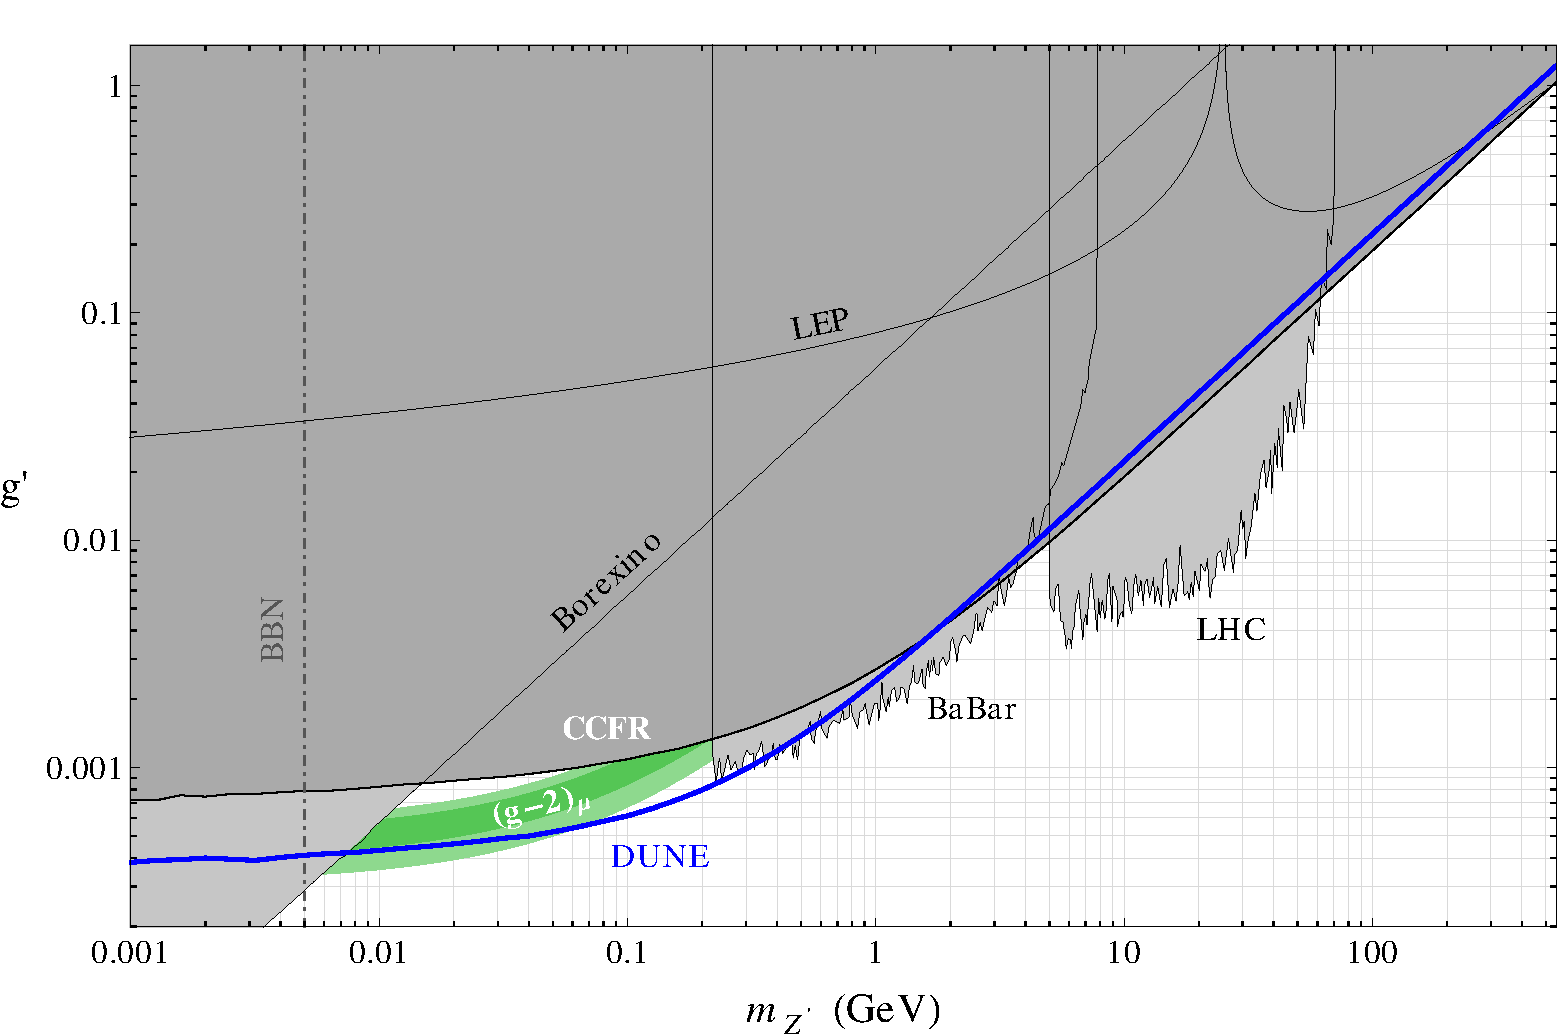
\includegraphics[width=0.7\textwidth]{LmuLtau.pdf}
\caption{Existing constraints and projected DUNE sensitivity in the $L_\mu - L_\tau$ parameter space. Shown in green is the region where the $(g-2)_\mu$ anomaly can be explained at the $2\sigma$ level. The parameter regions already excluded by existing constraints are shaded in gray and correspond to a CMS search for $pp \to \mu^+\mu^- Z' \to \mu^+\mu^-\mu^+\mu^-$~\cite{Sirunyan:2018nnz} (``LHC''), a BaBar search for $e^+e^- \to \mu^+\mu^- Z' \to \mu^+\mu^-\mu^+\mu^-$~\cite{TheBABAR:2016rlg} (``BaBar''), precision measurements of $Z \to \ell^+ \ell^-$ and $Z \to \nu\bar\nu$ couplings~\cite{ALEPH:2005ab,Altmannshofer:2014cfa} (``LEP''), a previous measurement of the trident cross section~\cite{Mishra:1991bv,Altmannshofer:2014pba} (``CCFR''), a measurement of the scattering rate of solar neutrinos on electrons~\cite{Bellini:2011rx,Harnik:2012ni,Agostini:2017ixy} (``Borexino''), and bounds from Big Bang Nucleosynthesis~\cite{Ahlgren:2013wba,Kamada:2015era} (``BBN''). The DUNE sensitivity shown by the solid blue line assumes a measurement of the trident cross section with $25\%$ precision.}
\label{fig:LmuLtau}
\end{figure}
%%%%%%%%%%%%%%%%%%%%%%%%%%%%%%%%%%%%%%%%%%%%%%%%%%%%%%%%%%%%%%%

In Fig.~\ref{fig:LmuLtau} we show the existing CCFR constraint on the model parameter space in the $m_{Z'}$ vs. $g'$ plane and compare it to the region of parameter space where the anomaly in $(g-2)_\mu = 2 a_\mu$ can be explained. The green region shows the $1\sigma$ and $2\sigma$ preferred parameter space corresponding to a shift $\Delta a_\mu = a_\mu^\text{exp}-a_\mu^\text{SM} = (2.71 \pm 0.73) \times 10^{-9}$~\cite{Keshavarzi:2018mgv}.
Shown are in addition constraints from LHC searches for the $Z'$ in the $pp \to \mu^+\mu^- Z' \to \mu^+\mu^-\mu^+\mu^-$ process~\cite{Sirunyan:2018nnz} (see also~\cite{Altmannshofer:2014pba}), direct searches for the $Z'$ at BaBar using the $e^+e^- \to \mu^+\mu^- Z' \to \mu^+\mu^-\mu^+\mu^-$ process~\cite{TheBABAR:2016rlg}, and constraints from LEP precision measurements of leptonic $Z$ couplings~\cite{ALEPH:2005ab,Altmannshofer:2014cfa}.  
Also a Borexino bound on non-standard contributions to neutrino-electron scattering~\cite{Harnik:2012ni,Bellini:2011rx,Agostini:2017ixy} has been used to constrain the $L_\mu - L_\tau$ gauge boson~\cite{Kamada:2015era,Araki:2015mya,Kamada:2018zxi}. Our reproduction of the Borexino constraint shown.
For very light $Z'$ masses of $O$(few MeV) and below, strong constraints from measurements of the effective number of relativistic degrees of freedom during Big Bang Nucleosynthesis (BBN) apply~\cite{Ahlgren:2013wba,Kamada:2015era}.
Taking into account all relevant constraints, parameter space to explain $(g-2)_\mu$ is left below the di-muon threshold $m_{Z'} \lesssim 210$~MeV.

%%% NEUTRINO TRIDENTS %%%%%%%%%%%%%%%%%%%%%%%%%%%%%%%%%%%%%%
%%%%%%%%%%%%%%%%%%%%%%%%%%%%%%%%%%%%%%%%%%%%%%%%%%%%%%%%%%%%



\clearpage
\section{Searches for NSI, Non-Unitarity, and CPT Symmetry Violation}
\subsection{Non-Standard Interactions (NSI)}
\label{sec:nsi}
Non-standard neutrino interactions can significantly modify the data to be collected by DUNE as long as the new physics parameters are large enough. NSI may impact the determination of current unknowns such as CP violation~\cite{Masud:2015xva,Masud:2016bvp}, mass hierarchy~\cite{Masud:2016gcl} and octant of $\theta_{23}$~\cite{Agarwalla:2016fkh}. If the DUNE data are consistent with the standard oscillation for three massive neutrinos, neutral-current (NC) NSI effects of order 0.1 $G_F$, affecting neutrino propagation through the Earth, can be ruled out at DUNE~\cite{deGouvea:2015ndi,Coloma:2015kiu}. We notice that DUNE might improve current constraints on $|\epsilon^m_{e \tau}|$ and $|\epsilon^m_{e \mu}|$ by a factor 2-5~\cite{Ohlsson:2012kf,Miranda:2015dra,Farzan:2017xzy}. New charged-current (CC) interactions can also lead to modifications in the production and the detection of neutrinos. The findings on source and detector NSI studies at DUNE are presented in~\cite{Blennow:2016etl,Bakhti:2016gic}. Particularly, the simultaneous impact on the measurement of $\delta_{\rm CP}$ and $\theta_{23}$ is investigated in detail. Depending on the assumptions, such as the use of the near detector and whether NSI at production and detection are the same, the impact of source/detector NSI at DUNE may be relevant. In this report we are assuming the results from~\cite{Blennow:2016etl} in which DUNE does not have sensitivity to discover or to improve bounds on source/detector NSIs to focus our attention in the propagation.

\subsubsection{NSI in propagation at DUNE}
%%%%%%%%%%%%%%%%%%%%%%%%%%%%%%%%%
%{\bf Authors: Chatterjee, Fernandez-Martinez, Forero, Guzzo, Kamiya, Miranda, Moura, Peres, Tortola, et al.}
Neutral current non-standard interactions (NC NSI) can be understood as non-standard
matter effects that are visible only in a far detector at a sufficiently long baseline. They can be parameterized as new contributions
to the MSW matrix in the neutrino-propagation Hamiltonian:
\begin{equation}
  H = U \left( \begin{array}{ccc}
           0 &                    & \\
             & \Delta m_{21}^2/2E & \\
             &                    & \Delta m_{31}^2/2E
         \end{array} \right) U^\dag + \tilde{V}_{\rm MSW} \,,
\end{equation}
with
\begin{equation}
  \tilde{V}_{\rm MSW} = \sqrt{2} G_F N_e
\left(
  \begin{array}{ccc}
    1 + \epsilon^m_{ee}       & \epsilon^m_{e\mu}       & \epsilon^m_{e\tau}  \\
        \epsilon^{m*}_{e\mu}  & \epsilon^m_{\mu\mu}     & \epsilon^m_{\mu\tau} \\
        \epsilon^{m*}_{e\tau} & \epsilon^{m*}_{\mu\tau} & \epsilon^m_{\tau\tau}
  \end{array} 
\right)
\label{eq:epsmatrix}
\end{equation}
Here, $U$ is the standard PMNS leptonic mixing matrix, for which we use the standard parameterization found, e.g., in~\cite{Agashe:2014kda}, and the $\epsilon$-parameters give the
magnitude of the NSI relative to standard weak interactions.  For new physics
scales of a few hundred GeV,  a value of $|\epsilon|$ of the order
%%%\lesssim 
0.01 or less is
expected~\cite{Davidson:2003ha,GonzalezGarcia:2007ib,Biggio:2009nt}. DUNE
%%%\kmadj{1300} 
baseline provides an advantage in the detection of NSI relative
to existing beam-based experiments with shorter baselines.
Only atmospheric-neutrino experiments have longer baselines, but the sensitivity
of these experiments to NSI is limited by systematic effects~\cite{Adams:2013qkq}.

To assess DUNE sensitivity to NC NSI, the NSI discovery reach
is defined in the following way: the expected event spectra are
simulated using GLoBES~\cite{Huber:2004ka,Huber:2007ji}, assuming \emph{true} values for the NSI
parameters, and a fit is then attempted assuming no NSI. If the fit is
incompatible with the simulated data at a given confidence level,
the chosen \emph{true} values of the NSI parameters are considered to be within the experimental discovery reach.

In this analysis, we use GLoBES with the Monte Carlo Utility Based Experiment Simulator (MonteCUBES) C library~\cite{Blennow:2009pk}, a plugin that replaces the deterministic GLoBES minimizer by a Markov Chain Monte Carlo (MCMC) method that is able to handle higher dimensional parameter spaces. In the simulations we use the configuration for the DUNE CDR~\cite{Alion:2016uaj}. Each point scanned by the MCMC is stored and a frequentist $\chi^2$ analysis is performed with the results.

Considering that NSI exists, conducting the analysis with all the NSI parameters free to vary, we obtain the sensitivity regions in figure~\ref{fig:nsi}. We omit the superscript $m$ that appears in equation~\ref{eq:epsmatrix}. 
The credible regions are given in terms of percent Confidence Level (CL).
\begin{figure}[!htb]
	\centering
    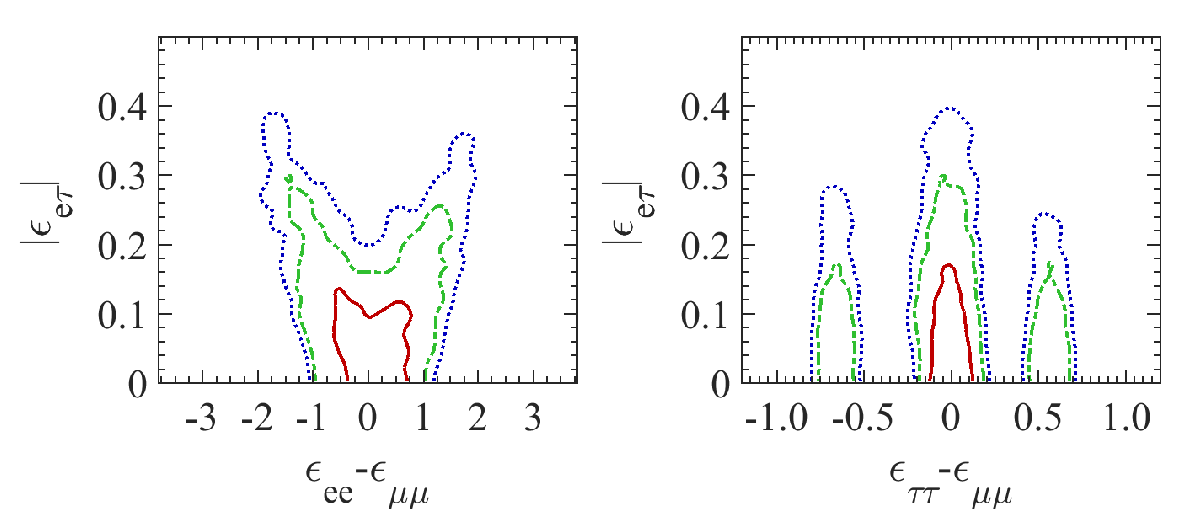
\includegraphics[width=0.6\columnwidth]{graphics/TDR12.pdf}
    
    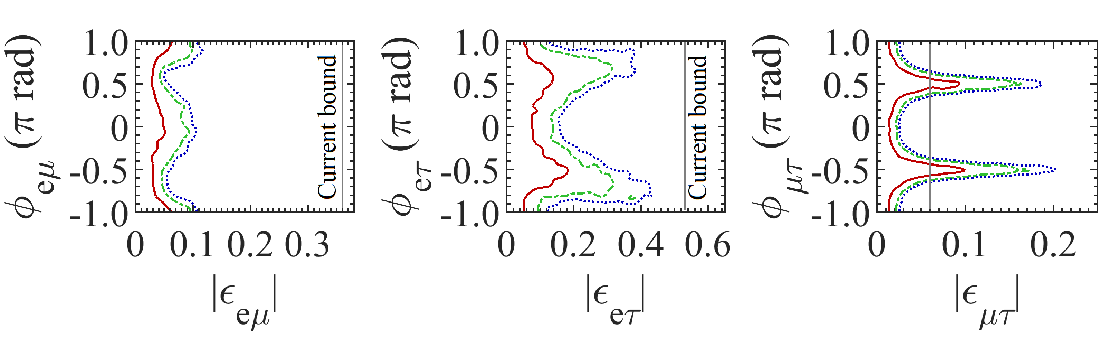
\includegraphics[width=0.75\columnwidth]{graphics/TDR4.pdf}
   \caption[NSI parameters. Allowed regions.]{\label{fig:nsi}Allowed regions of the non-standard oscillation parameters in which we see important degeneracies (top) and the complex non-diagonal ones (bottom). We conduct the analysis considering all the NSI parameters non-negligible. The sensitivity regions are for 68\% (red line (left)), 90\% (green dashed line (middle)), and 95\% CL (blue dotted line (right)). Current bounds are taken from~\cite{Gonzalez-Garcia:2013usa}.}
\end{figure}
We note, however, that constraints on $\epsilon_{\tau\tau}-\epsilon_{\mu\mu}$ coming from global fit analysis~\cite{Gonzalez-Garcia:2013usa,Miranda:2015dra,Farzan:2017xzy,Esteban:2018ppq} can remove the left and right solutions of $\epsilon_{\tau\tau}-\epsilon_{\mu\mu}$ in figure~\ref{fig:nsi}.

In order to constrain the standard oscillation parameters when NSI is present, we use the fit for three neutrino mixing from~\cite{Gonzalez-Garcia:2013usa} and implement prior constraints to restrict the region sampled by the MCMC. The sampling of the parameter space is explained in~\cite{Coloma:2015kiu} and the priors that we use can be found in table~\ref{tab:priors1}.
\begin{table}[htb]
\caption{Oscillation parameters and priors implemented with the MCMC calculating figure~\ref{fig:nsi}.} \label{tab:priors1}
\begin{center}
\begin{tabular}{cccc}
\hline
\hline
Parameter&Nominal&1$\sigma$ range ($\pm$)\\ 
\hline
$\theta_{12}$ &0.19$\pi~\textrm{rad}$&2.29\%\\
$\sin^2(2\theta_{13})$ &0.08470&0.00292\\
$\sin^2(2\theta_{23})$ &0.9860&0.0123\\
$\Delta m^2_{21} $ &7.5 $\times10^{-5}\textrm{eV}^2$&2.53\%\\
$\Delta m^2_{31} $ &2.524 $\times10^{-3}\textrm{eV}^2$&free\\
$\delta_{\rm CP} $ &1.45$\pi~\textrm{rad}$&free\\
\hline 
\hline
\end{tabular}
\end{center}
\end{table}

Then we can observe the effects of NSI on the measurements of the standard oscillation parameters at DUNE. In figure~\ref{fig:standar-nsi}, we superpose the allowed regions with non-negligible NSI and the standard-only credible regions at 90\% CL. There is an important degeneracy that appears in the measurement of the mixing angle $\theta_{23}$. We also see that the sensitivity of the CP phase is strongly affected.
\begin{figure}[!htb]
	\centering
    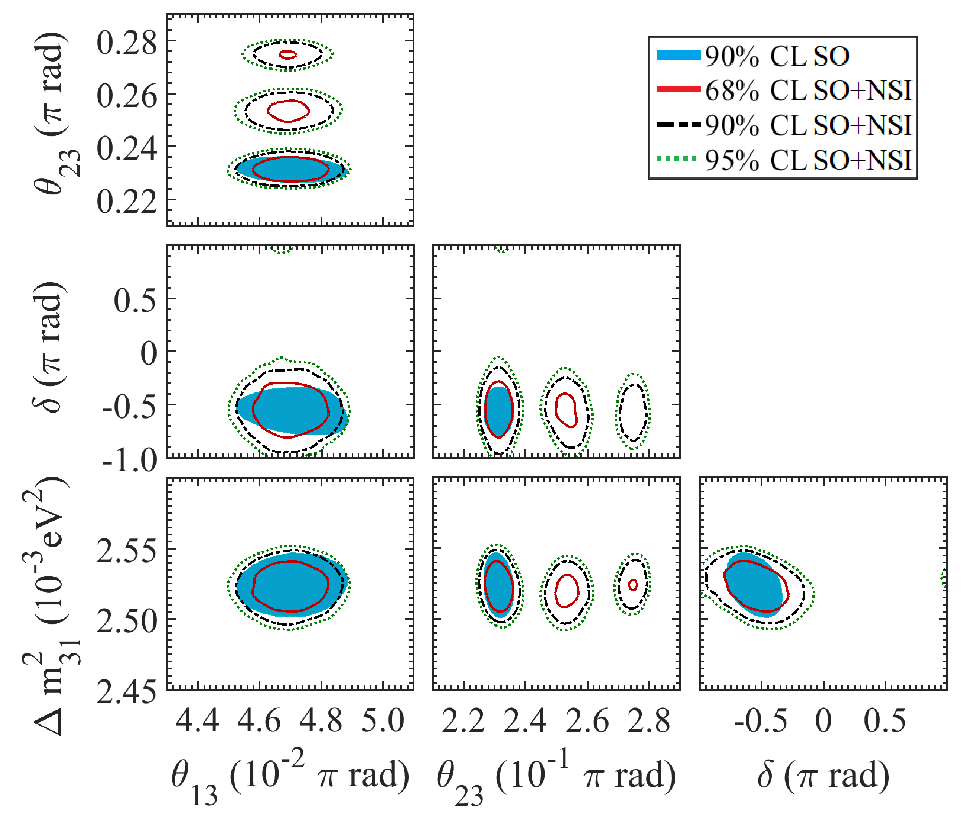
\includegraphics[width=0.6\columnwidth]{graphics/TDR10.pdf}
   \caption[]{\label{fig:standar-nsi}Projections of the standard oscillation parameters considering NSI is possible. The sensitivity regions are for 68\%, 90\%, and 95\% CL. The allowed regions considering negligible NSI (standard oscillation (SO)) are superposed to the SO+NSI at 90\% CL.}
\end{figure}

%%%%%%%%%%%%%%%%%%%%%%%%%%%%%%%%%%%%%%%%%%%%%%%%%%%%%%%%%%%%%%
\subsubsection{Effects of baseline and matter density variation on NSI measurements}\label{ssec:matter}
%%%%%%%%%%%%%%%%%%%%%%%%%%%%%%%%%%%%%%%%%%%%%%%%%%%%%%%%%%%%%%
The effects of matter density variation and its average along the beam path from Fermilab to SURF were studied considering the standard neutrino oscillation framework with three flavors~\cite{Roe:2017zdw,Kelly:2018kmb}. In order to obtain the results of figures~\ref{fig:nsi} and~\ref{fig:standar-nsi}, we use a high precision calculation for the baseline of 1284.9~km and the average density of 2.8482~g/cm$^3$~\cite{Roe:2017zdw}.

The DUNE collaboration has been using the so-called PREM~\cite{Dziewonski:1981xy,PREM2} density profile to consider matter density variation. With this assumption, the neutrino beam crosses a few constant density layers.
However, a more detailed density map is available for the USA with more than 50 layers and $0.25 \times 0.25$ degree cells of latitude and longitude: The Shen-Ritzwoller or S.R. profile~\cite{SR:2016,Roe:2017zdw}. Comparing the S.R. with the PREM profiles, Kelly and Parke~\cite{Kelly:2018kmb} show that, in the standard oscillation paradigm, DUNE is not highly sensitive to the density profile and that the only oscillation parameter with its measurement slightly impacted by the average density true value is $\delta_{\rm CP}$.
NSI, however, may be sensitive to the profile, particularly considering the phase $\phi_{e\tau}$~\cite{Chatterjee:2018dyd}, to which DUNE will have a high sensitivity~\cite{Ohlsson:2012kf,Miranda:2015dra,deGouvea:2015ndi,Coloma:2015kiu,Farzan:2017xzy}, as we also see in figure~\ref{fig:nsi}.

\subsubsection{Conclusions and prospects}
NSI can significantly impact the determination of current unknowns such as CP violation and the octant of $\theta_{23}$. Clean determination of intrinsic CP phase at long baseline experiments such as DUNE is a formidable task~\cite{Rout:2017udo}. A feasible strategy to extricate physics scenarios at DUNE using high energy beams was suggested in ~\cite{Masud:2017bcf}.

\subsection{Non-Unitarity (NU)}
%%%%%%%%%%%%%%%%%%%%%%%%%%%%%%%%%%%
%{\bf Authors: Fernandez-Martinez, Forero, Miranda, Tórtola
%\vspace{0.5cm}
A generic characteristic of most models explaining the neutrino mass
pattern is the presence of heavy neutrino states, beyond the
three light states of the Standard Model of particle
physics~\cite{Minkowski:1977sc,Mohapatra:1979ia,Yanagida:1979as,GellMann:1980vs}. This implies a deviation from unitarity of the $3\times3$ PMNS matrix, which can be particularly sizable the lower the mass of the extra states are~\cite{Mohapatra:1986bd,Akhmedov:1995vm,Akhmedov:1995ip,Malinsky:2005bi}.
For values of non-unitarity parameter deviations of order $10^{-2}$, this would decrease the expected reach of DUNE to the standard parameters, although stronger bounds existing from charged leptons would be able to restore its expected performance~\cite{Blennow:2016jkn,Escrihuela:2016ube}.

A generic characteristic of most models explaining the neutrino mass
pattern is the presence of heavy neutrino states, additional to the
three light states of the Standard Model of particle
physics~\cite{Mohapatra:1998rq,Valle:2015pba,Fukugita:2003en}. These
types of models will imply that the $3\times3$ PMNS matrix is not
unitary due to the mixing with the additional states.  Besides the
type-I seesaw
mechanism~\cite{GellMann:1980vs,Yanagida:1979as,Mohapatra:1979ia,Schechter:1980gr},
different low-scale seesaw models include right-handed neutrinos that
are relatively not-so-heavy~\cite{Mohapatra:1986bd} and perhaps
detectable at collider experiments.

These additional heavy leptons would mix with the light neutrino
states and, as a result, the complete unitary mixing matrix will be a
squared $n \times n$ matrix, with $n$ the total number of neutrino
states. As a result, the usual $3\times 3$ PMNS matrix, which we will dub $N$ to stress its non-standard nature, will be
non-unitary. One of the possible general ways to parameterize these unitarity deviations in $N$ is through a triangular matrix~\cite{Escrihuela:2015wra}~\footnote{For a similar parameterization corresponding to a $(3+1)$ and a $(3+3)$-dimensional mixing matrix,  see Refs.~\cite{Xing:2007zj,Xing:2011ur}}
%%
 \begin{equation}
  N = 
 \left\lgroup
 \begin{array}{ccc} 
 1-\alpha_{ee} & 0 & 0 \\
 \alpha_{\mu e} & 1-\alpha_{\mu \mu} & 0 \\
  \alpha_{\tau e} & \alpha_{\tau \mu} & 1-\alpha_{\tau \tau}
 \end{array}
 \right \rgroup U \,,
 \label{eq:triangular}
 \end{equation}
 % 
with $U$ a unitary matrix that tends to the usual PMNS matrix when the non-unitary parameters $\alpha_{ij} \rightarrow 0$~\footnote{The original parameterization in ref.~\cite{Escrihuela:2015wra} uses $\alpha_{ii}$ instead of $\alpha_{\beta\gamma}$. The equivalence between the two notations is as follows: $\alpha_{ii} = 1-\alpha_{\beta\beta}$ and $\alpha_{ij} = \alpha_{\beta\gamma}$.} .
%
 The triangular
matrix in this equation accounts for the non-unitarity of the $3\times 3$ matrix for any number of extra neutrino species. This parametrization has been shown to be particularly well-suited for oscillation searches~\cite{Escrihuela:2015wra,Blennow:2016jkn} since, compared to other alternatives, it minimizes the departures of its unitary component $U$ from the mixing angles that are directly measured in neutrino oscillation experiments when unitarity is assumed.

The phenomenological implications of a non-unitary leptonic mixing matrix have been extensively studied in flavour and electroweak precision observables as well as in the neutrino oscillation phenomenon~\cite{Shrock:1980vy,Schechter:1980gr,Shrock:1980ct,Shrock:1981wq,Langacker:1988ur,Bilenky:1992wv,Nardi:1994iv,Tommasini:1995ii,Antusch:2006vwa,FernandezMartinez:2007ms,Antusch:2008tz,Biggio:2008in,Antusch:2009pm,Forero:2011pc,Alonso:2012ji,Antusch:2014woa,Abada:2015trh,Fernandez-Martinez:2015hxa,Escrihuela:2015wra,Parke:2015goa,Miranda:2016wdr,Fong:2016yyh,Escrihuela:2016ube}. For recent global fits to all flavour and electroweak precision data summarizing present bounds on non-unitarity see Refs.~\cite{Antusch:2014woa,Fernandez-Martinez:2016lgt}. 

%%%%%%%%%%%%%%%%%%%%%
\begin{table}[htb]
\caption{\label{tab:bounds} Expected $90 \%$~CL constraints on the non-unitarity parameters $\alpha$ from DUNE. }
\begin{center}
\renewcommand{\arraystretch}{1.6}
\begin{tabular}{  l@{\quad\quad}  c@{\quad\quad}   c@{\quad\quad}   c@{\quad\quad}      }
\hline
$\alpha_{ee}$ & $0.3$ & $\alpha_{\mu e}$ & $0.04$  \\
$\alpha_{\mu\mu}$ & $0.2$ & $\alpha_{\tau e}$ & $0.7$ \\
$\alpha_{\tau\tau}$ & $0.8$ & $\alpha_{\tau\mu}$ & $0.2$  \\ \hline
\end{tabular}
\end{center}
\end{table}
%%%%%%%%%%%%%%%%%%%%%

\subsubsection{NU constraints from DUNE}
Recent studies have shown that DUNE can constrain the non-unitarity parameters~\cite{Blennow:2016jkn, Escrihuela:2016ube}. The summary of the $90 \%$~CL bounds on the different $\alpha_{ij}$ elements profiled over all other parameters is given in table~\ref{tab:bounds}.
These bounds are comparable with other constraints from present oscillation experiments, although they are not competitive with those obtained from flavour and electroweak precision data.
For this analysis, and the ones that will be presented below, we have used the GLoBES software~\cite{Huber:2004ka,Huber:2007ji} with the DUNE CDR configuration presented in ref.~\cite{Alion:2016uaj}. The standard (unitary) oscillation parameters have also been treated as in~\cite{Alion:2016uaj}. The unitarity deviations have been included both by an independent code (used to obtain the results shown in ref.~\cite{Escrihuela:2016ube}) and via the MonteCUBES~\cite{Blennow:2009pk} plug-in to cross validate our results.

\subsubsection{NU impact on DUNE standard searches}
Conversely, the presence of non-unitarity may affect the determination of the
Dirac CP-violating phase $\delta_{CP}$ in long-baseline experiments~\cite{Miranda:2016wdr,Fernandez-Martinez:2016lgt,Escrihuela:2016ube}.
 Indeed, when allowing for unitarity deviations, the expected CP discovery potential for DUNE could be significantly reduced.
However, the situation is alleviated when a combined analysis with the constraints on non-unitarity from other experiments is considered. This is illustrated in figure~\ref{fig:CPsens}. In the left panel, the discovery potential for CP violation is computed when the non-unitarity parameters introduced in Eq.~(\ref{eq:triangular}) are allowed in the fit. While for the Asimov data all $\alpha_{ij}=0$, the non-unitary parameters are allowed to vary in the fit with $1 \sigma$ priors of $10^{-1}$, $10^{-2}$ and $10^{-3}$ for the dotted green, dashed blue and solid black lines respectively. For the dot-dashed red line no prior information on the non-unitarity parameters has been assumed. As can be observed, without additional priors on the non-unitarity parameters, the capabilities of DUNE to discover CP violation from $\delta_{CP}$ would be seriously compromised~\cite{Escrihuela:2016ube}. However, with priors of order $10^{-2}$ matching the present constraints from other neutrino oscillation experiments~\cite{Escrihuela:2016ube,Blennow:2016jkn}, the standard sensitivity is almost recovered. If the more stringent priors of order $10^{-3}$ stemming from flavour and electroweak precision observables are added~\cite{Antusch:2014woa,Fernandez-Martinez:2016lgt}, the standard sensitivity is obtained.   

The right panel of figure~\ref{fig:CPsens} concentrates on the impact of the phase of the element $\alpha_{\mu e}$ in the discovery potential of CP violation from $\delta_{CP}$, since this element has a very important impact in the $\nu_e$ appearance channel. In this plot the modulus of $\alpha_{ee}$, $\alpha_{\mu \mu}$ and $\alpha_{\mu e}$ have been fixed to $10^{-1}$, $10^{-2}$, $10^{-3}$ and 0 for the dot-dashed red, dotted green, dashed blue and solid black lines respectively. All other non-unitarity parameters have been set to zero and the phase of $\alpha_{\mu e}$ has been allowed to vary both in the fit and in the Asimov data, showing the most conservative curve obtained. As for the right panel, it can be seen that a strong deterioration of the CP discovery potential could be induced by the phase of $\alpha_{\mu e}$ (see ref.~\cite{Escrihuela:2016ube}). However, for unitarity deviations of order $10^{-2}$, as required by present neutrino oscillation data constraints, the effect is not too significant in the range of $\delta_{CP}$ for which a $3 \sigma$ exclusion of CP conservation would be possible and it becomes negligible if the stronger $10^{-3}$ constraints from flavour and electroweak precision data are taken into account.  

Similarly, the presence of non-unitarity worsens degeneracies involving $\theta_{23}$, making the determination of the octant or even its maximality challenging.
This situation is shown in figure~\ref{fig:octant} where an input value of $\theta_{23} = 42.3^\circ$ was assumed. As can be seen, the fit in presence of non-unitarity (solid lines) introduces degeneracies for the wrong octant and even for maximal mixing~\cite{Blennow:2016jkn}. However, these degeneracies are solved upon the inclusion of present priors on the non-unitarity parameters from other oscillation data (dashed lines) and a clean determination of the standard oscillation parameters following DUNE expectations is again recovered.   

\begin{figure}[!t]
\centering
 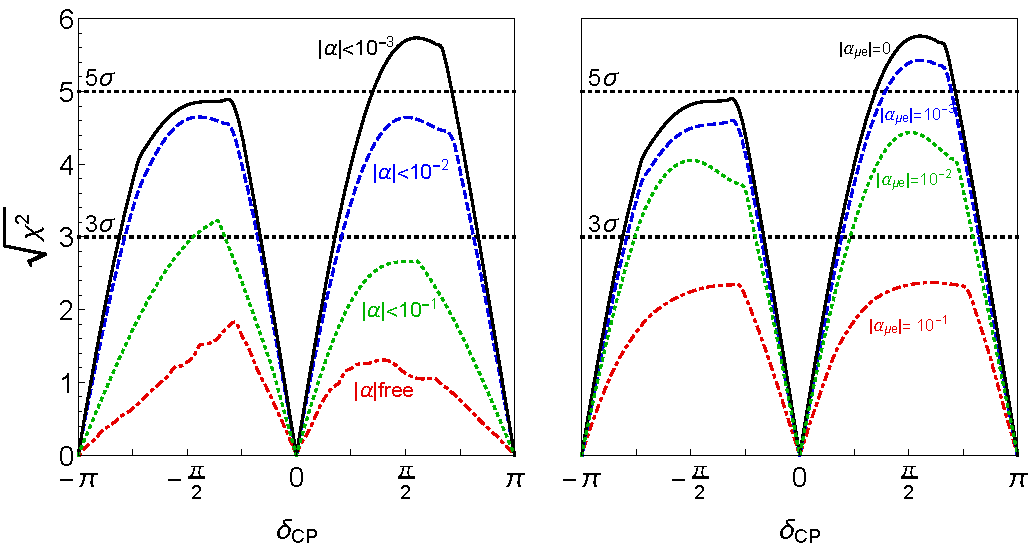
\includegraphics[width=0.8\columnwidth]{graphics/cpsens-comb.pdf}
\caption{The impact of non-unitarity on the DUNE CP violation discovery potential. See the text for details.}
\label{fig:CPsens}
\end{figure}

\begin{figure}
 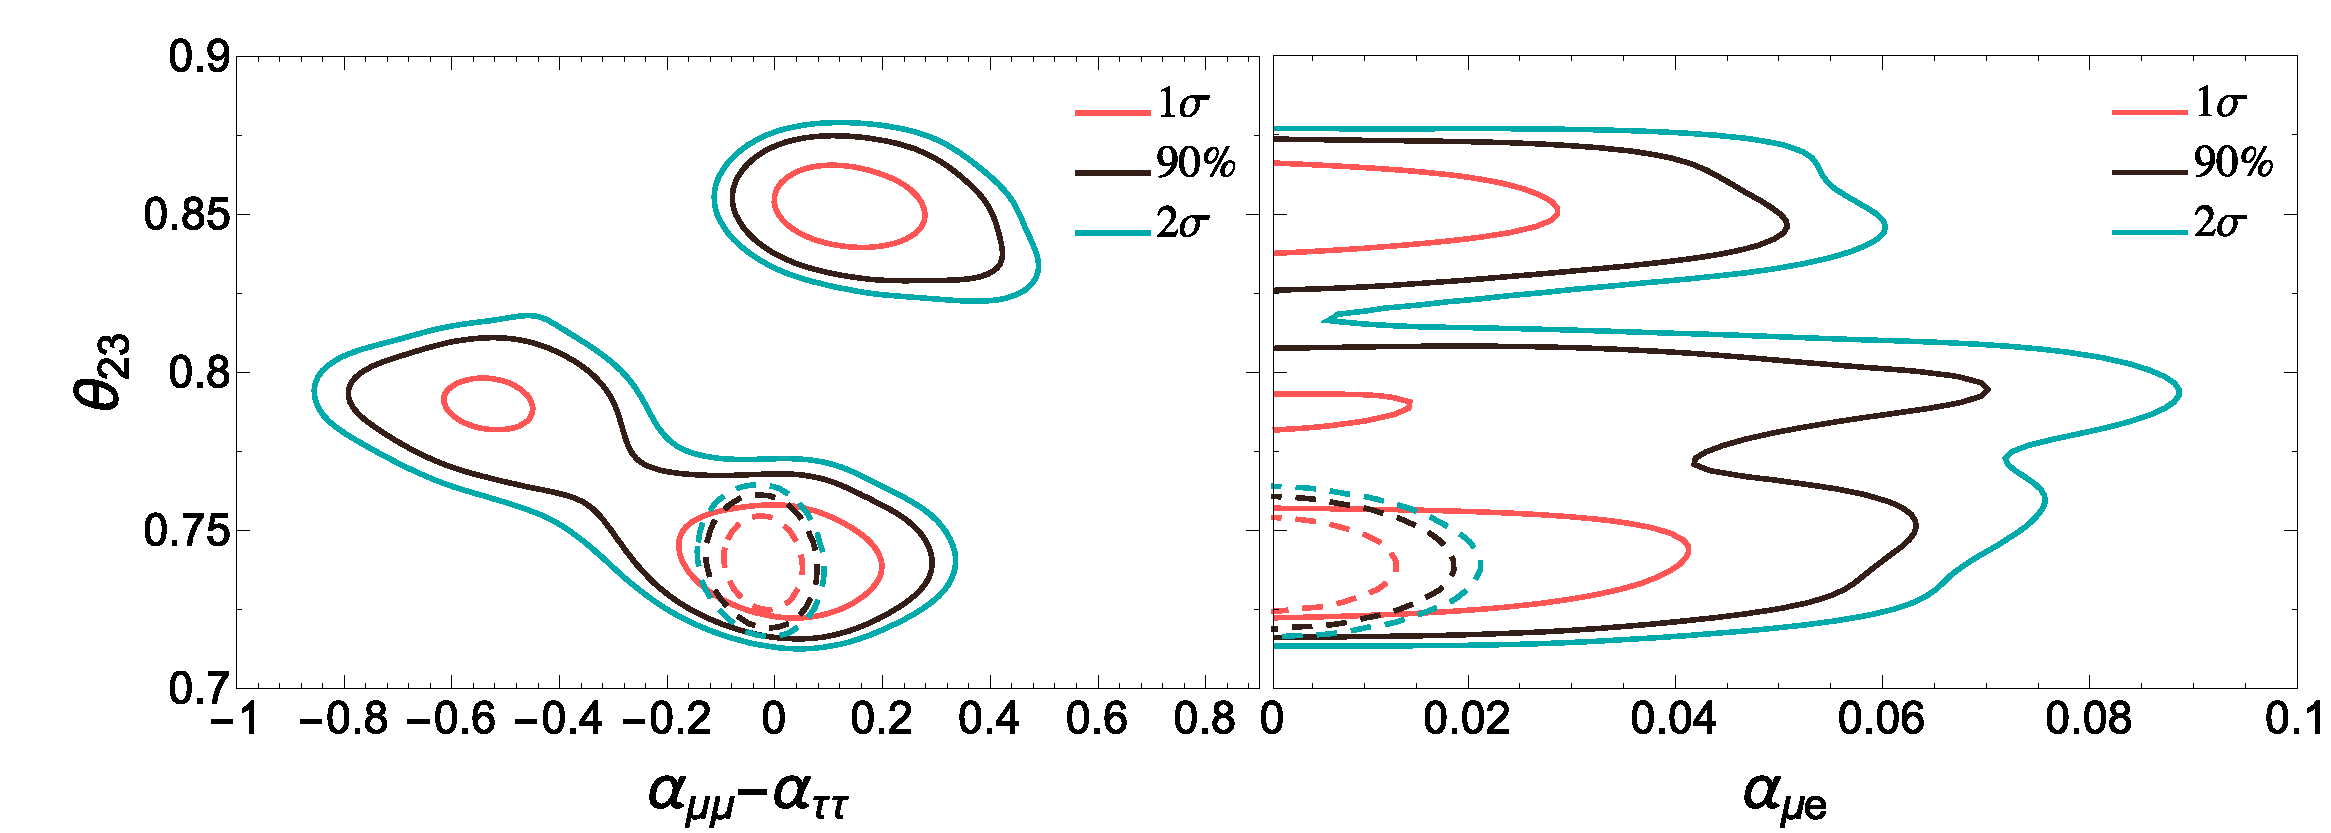
\includegraphics[width=0.8\columnwidth]{graphics/combined_pdf.pdf} 
 \begin{center}
  \caption{Expected frequentist allowed regions at the $1 \sigma$,
    $90\%$ and $2 \sigma$ CL\ for DUNE. All new physics parameters
    are assumed to be zero so as to obtain the expected
    non-unitarity sensitivities. The solid
    lines correspond to the analysis of DUNE data alone, while the
    dashed lines include the present constraints on non-unitarity.
\label{fig:octant}}
 \end{center}
\end{figure}

\subsubsection{Conclusions}
A non-unitary lepton mixing matrix, as generally expected from the most common extensions of the Standard Model explaining neutrino masses, would affect the neutrino oscillations to be measured by DUNE. The sensitivity that DUNE would provide to the non-unitarity parameters is comparable to that from present oscillation experiments, while not competitive to that from flavour and electroweak precision observables, which is around an order of magnitude more stringent. Conversely, the capability of DUNE to determine the standard oscillation parameters such as CP violation from $\delta_{CP}$ or the octant or maximality of $\theta_{23}$ would be seriously compromised by unitarity deviations in the PMNS. This negative impact is however significantly reduced when priors on the size of these deviations from other oscillation experiments are considered and disappears altogether if the more stringent constraints from flavour and electroweak precision data are added instead.

\subsection{CPT Symmetry Violation}
%%%%%%%%%%%%%%%%%%%%%%%%%%%%%%%%%%%
%{\bf Authors: Barenboim, Ternes, and Tórtola.}
%\vspace{0.5cm}
CPT symmetry, the combination of Charge Conjugation, Parity and Time reversal, is a corner-stone of our model building strategy.
%and therefore the repercussions of its potential violation would severely threaten the standard model of particle physics. 
DUNE can improve the present limits on Lorentz and CPT violation by several orders of magnitude~\cite{Streater:1989vi,Barenboim:2002tz,Kostelecky:2003cr,Diaz:2009qk,Kostelecky:2011gq,Barenboim:2017ewj}, contributing as very important experiment to test one of the deepest results of quantum field theory.
%
CPT invariance is surely one of the predictions of major importance of local, relativistic quantum field theory. One of the predictions of CPT invariance is that particles and antiparticles have the same masses and, if unstable, the same lifetimes. To prove the CPT theorem one needs only three ingredients~\cite{Streater:1989vi}: Lorentz invariance, Hermiticity of the Hamiltonian, and Locality.
%
%If CPT turned out to be violated, the effect on modern fundamental particle physics would be gigantic. We would have to rethink our model-building strategies, since one of the three ingredients above  would not hold anymore.  

Experimental bounds on CPT invariance can be derived using the neutral kaon system~\cite{Schwingenheuer:1995uf}:
%
\begin{equation}
  \frac{|m(K^0) - m(\overline{K}^0)|}{m_K} < 0.6 \times 10^{-18}\,. 
  \label{eq:mK}
\end{equation}
%
This result, however, should be interpreted very carefully because of two reasons: first, we do not have a complete theory of CPT violation. Therefore, it is rather arbitrary to take the kaon-mass as a scale. Second, since kaons are bosons, the term entering the Lagrangian is the mass squared and not the mass itself. Having this in mind, we can rewrite the previous bound as:
%
%\begin{equation}
 $ |m^2(K^0) - m^2(\overline{K}^0)| < 0.3~\mbox{eV}^2 \, $.
%  \label{eq:mK2}
%\end{equation}
%
Here we will see that neutrinos can test the predictions of the CPT theorem to an unprecedented extent and could, therefore, provide stronger limits than the ones regarded as the most stringent ones by now\footnote{CPT was tested also using charged leptons. However, these measurements involve a combination
of mass and charge and are not a direct CPT test. Only neutrinos can provide CPT tests on an elementary mass not contaminated by charge.}. 
%
In the absence of a solid model of flavor, not to mention one of CPT violation, the spectrum  of neutrinos and antineutrinos can differ both  in the mass eigenstates themselves as well as in the flavour composition of each of these states. It is important to notice then that neutrino oscillation experiments can  only test CPT in the mass differences and mixing angles. An overall shift between the neutrino and antineutrino spectra will be missed by oscillation experiments.  Nevertheless, such a pattern can be bounded by cosmological data, see ref.~\cite{Barenboim:2017vlc}. Unfortunately direct searches for neutrino mass (past, present, and future) involve only antineutrinos and therefore 
cannot be used to draw any conclusion on  CPT invariance on the absolute mass scale either.
%
Therefore, using neutrino oscillation data, we will compare the mass splittings and mixing angles of  neutrinos with those of antineutrinos. Differences in the neutrino and antineutrino spectrum would imply the violation of the CPT theorem.
%Let us stress, however, that without an explicit model for CPT violation it is not straightforward or even meaningful to compare the neutrino-antineutrino mass squared differences and the kaon ones\footnote{Note that we are not considering any particular model of CPT violation and, then, the results presented can be regarded as model-independent.}. CPT violation may show up only in one of the sectors and therefore the strong bounds in one of them might not be directly applicable to the other. Nevertheless, there are reasons to believe that neutrinos are an ideal candidate to test CPT violation: quantum gravity is assumed to be non-local, opening the door to a potential CPT violation. Its effects, however, are expected to be Planck suppressed, i.e., $\left\langle v\right\rangle^2/M_{\text{P}} $, where $v$ is the higgs vev, exactly in the right ballpark for neutrino experiments to see them. Also, neutrinos are typically thought to obtain their mass through the see-saw mechanism, which requires neutrinos have a Majorana mass.  Such a mass term requires new physics and a new scale where non-locality may show up, potentially making neutrinos uniquely sensitive to CPT violation.

In ref.~\cite{Barenboim:2017ewj} the authors derived the most up-to-date bounds on CPT invariance from the neutrino sector. The data used to derive these bounds are the same considered in the global fit to neutrino oscillations in ref.~\cite{deSalas:2017kay}. Of course, experiments which cannot distinguish between neutrinos and antineutrinos, such as atmospheric data from Super-Kamiokande~\cite{Abe:2017aap}, IceCube-DeepCore~\cite{Aartsen:2014yll,Aartsen:2017nmd} and ANTARES~\cite{AdrianMartinez:2012ph} were not included. The complete data set used, as well as the parameters to which they are sensitive are the following:
%
%\begin{itemize}
 1. from solar neutrino data~\cite{Cleveland:1998nv,Kaether:2010ag,Abdurashitov:2009tn,hosaka:2005um,Cravens:2008aa,Abe:2010hy,Nakano:PhD,Aharmim:2008kc,Aharmim:2009gd,Bellini:2013lnn}:  $\theta_{12}$, $\Delta m_{21}^2$, and $\theta_{13}$;
 2. from neutrino mode in long--baseline experiments K2K~\cite{Ahn:2006zza}, MINOS~\cite{Adamson:2013whj,Adamson:2014vgd}, T2K~\cite{Abe:2017uxa,Abe:2017bay}, and NO$\nu$A~\cite{Adamson:2017qqn,Adamson:2017gxd}:  $\theta_{23}$, $\Delta m_{31}^2$, and $\theta_{13}$;
 3. from KamLAND reactor antineutrino data~\cite{Gando:2010aa}: $\overline{\theta}_{12}$, $\Delta \overline{m}_{21}^2$, and $\overline{\theta}_{13}$;
 4. from short-baseline reactor antineutrino experiments Daya Bay~\cite{An:2016ses}, RENO~\cite{RENO:2015ksa}, and Double Chooz~\cite{Abe:2014bwa}:     $\overline{\theta}_{13}$ and $\Delta \overline{m}_{31}^2$;
 5. from antineutrino mode in long-baseline experiments MINOS~\cite{Adamson:2013whj,Adamson:2014vgd} and T2K~\cite{Abe:2017uxa,Abe:2017bay}: $\overline{\theta}_{23}$, $\Delta \overline{m}_{31}^2$, and
$\overline{\theta}_{13}$~\footnote{The K2K experiment took  data only in neutrino mode, while the NO$\nu$A experiment has not published data in the antineutrino mode yet.}.\\
%\end{itemize}
%
From the analysis of all previous data samples, one can derive the most up-to-date bounds on CPT violation:
%
% \begin{eqnarray}
$ |\Delta m_{21}^2-\Delta \overline{m}_{21}^2| < 4.7\times 10^{-5} \,  \text{eV}^2,\,\,
%  \nonumber \\
 |\Delta m_{31}^2-\Delta \overline{m}_{31}^2| < 3.7\times 10^{-4} \, \text{eV}^2,\,\,
% \nonumber \\
 |\sin^2\theta_{12}-\sin^2\overline{\theta}_{12}| < 0.14\,,\,\,
%  \\
 |\sin^2\theta_{13}-\sin^2\overline{\theta}_{13}| < 0.03\,, \,\,
%  \nonumber \\
 {\rm and}~|\sin^2\theta_{23}-\sin^2\overline{\theta}_{23}| < 0.32\,.
 $ \\
 %\nonumber.
% \label{eq:new-bounds}
% \end{eqnarray} 
%
At the moment it is not possible to set any bound on $|\delta-\overline{\delta}|$, since all possible values of
$\delta$ or $\overline{\delta}$ are allowed by data. The preferred intervals of $\delta$ obtained in ref.~\cite{deSalas:2017kay} can only be obtained after combining the neutrino and antineutrino data samples. 
The limits  on $\Delta(\Delta m_{31}^2)$ and $\Delta(\Delta m_{21}^2)$  are already better than the one derived from the neutral kaon system and should be regarded as the best bounds on CPT violation on the mass squared so far. Note that these results were derived assuming the same mass ordering for neutrinos and antineutrinos. If the ordering was different for neutrinos and antineutrinos, this would be an indication for CPT violation on its own. In the following we show how DUNE could improve this bound.

\subsubsection{Sensitivity to CPT symmetry violation in the neutrino sector}
\label{sec:sensitivity}

\begin{table}[htb]\centering
%  \catcode`?=\active \def?{\hphantom{0}}
\caption{Oscillation parameters used to simulate neutrino and antineutrino data analyzed in subsection~\ref{sec:sensitivity}.}
     \label{tab:par2}
   \begin{tabular}{lc}
    \hline
    parameter & value 
    \\
    \hline
    $\Delta m^2_{21}$& $7.56\times 10^{-5}\text{eV}^2$\\  
    %%
    $\Delta m^2_{31}$&  $2.55\times 10^{-3}\text{eV}^2$\\
    %%	
    $\sin^2\theta_{12}$ & 0.321\\ 
     $\sin^2\theta_{23}$ &  0.43, 0.50, 0.60\\
    $\sin^2\theta_{13}$ & 0.02155\\
   $\delta$ & 1.50$\pi$\\
       \hline
       \hline
     \end{tabular}
%       \captionsetup{justification=centering}
\end{table}

Here we study the sensitivity of the DUNE experiment to measure CPT violation in the neutrino sector, by analyzing neutrino and antineutrino oscillation parameters separately. We assume the neutrino oscillations being parameterized by the usual PMNS matrix $U_{\text{PMNS}}$, with parameters $\theta_{12},\theta_{13},\theta_{23},\Delta m_{21}^2,\Delta m_{31}^2, {\rm and}~\delta$, while the antineutrino oscillations are parameterized by a matrix $\overline{U}_{\text{PMNS}}$ with parameters $\overline{\theta}_{12},\overline{\theta}_{13},\overline{\theta}_{23},\Delta \overline{m}_{21}^2,\Delta \overline{m}_{31}^2, {\rm and}~\overline{\delta}$. Hence, antineutrino oscillation is described  by the same probability functions as neutrinos with the neutrino parameters replaced by their antineutrino counterparts~\footnote{Note that the antineutrino oscillation probabilities also include the standard change of sign in the CP phase.}. 
To simulate the future neutrino data signal in DUNE, in this section we assume the true values for neutrinos and antineutrinos to be the ones in table~\ref{tab:par2}.
Then, in the statistical analysis, we vary freely all the oscillation parameters, except the solar ones, which are fixed to their best fit values throughout the simulations. Given the great precision in the determination of the reactor mixing angle by the short-baseline reactor experiments~\cite{An:2016ses,RENO:2015ksa,Abe:2014bwa}, in our analysis we use a prior on $\overline{\theta}_{13}$, but not on $\theta_{13}$. We also consider three different values for the atmospheric angles, as indicated in table~\ref{tab:par2}. 

Therefore, to test the sensitivity at DUNE we perform the simulations assuming $\Delta x = |x-\overline{x}| = 0$, where $x$ is any of the oscillation parameters. Then we estimate the sensitivity to $\Delta x\neq 0$. To do so we calculate two $\chi^2$-grids, one for neutrinos and another one for antineutrinos, varying the four parameters of interest. After minimizing over all parameters except $x$ and $\overline{x}$, we calculate 
%
\begin{equation}
 \chi^2(\Delta x) = \chi^2(|x-\overline{x}|) = \chi^2(x)+\chi^2(\overline{x}),
 \label{eq:chi2-nu-nubar}
\end{equation}
%
where we have considered all the possible combinations of $|x-\overline{x}|$. The results are presented in figure~\ref{fig:sensitivity-CPT}, where we plot three different lines, labelled as "high", "max" and "low". These refer to the assumed value for the atmospheric angle: in the lower octant (low), maximal mixing (max) or in the upper octant (high). Here we can see that there is no sensitivity neither to $\Delta(\sin^2\theta_{13})$, where the 3$\sigma$ bound would be of the same order of the current measured value for $\sin^2\overline{\theta}_{13}$, nor to $\Delta\delta$, where no single value of the parameter would be excluded at more than 2$\sigma$.

On the contrary, interesting results for $\Delta(\Delta m_{31}^2)$ and $\Delta(\sin^2\theta_{23})$ are obtained. First, we see that  DUNE can put stronger bounds on the difference of the atmospheric mass splittings, namely $\Delta(\Delta m_{31}^2) < 8.1\times 10^{-5}$, improving the current neutrino bound by one order of magnitude. For the atmospheric angle, we obtain different results depending on the true value assumed in the simulation of DUNE data. In the lower right panel of figure~\ref{fig:sensitivity-CPT} we see the different behaviour obtained for $\theta_{23}$ lying in the lower octant, being maximal and lying in the upper octant. As one might expect, the sensitivity increases with $\Delta\sin^2\theta_{23}$ in the case of maximal mixing. However, if the true value lies in the lower or upper octant, a degenerate solution appears in the complementary octant.
\begin{figure}[!htb]
 \centering
        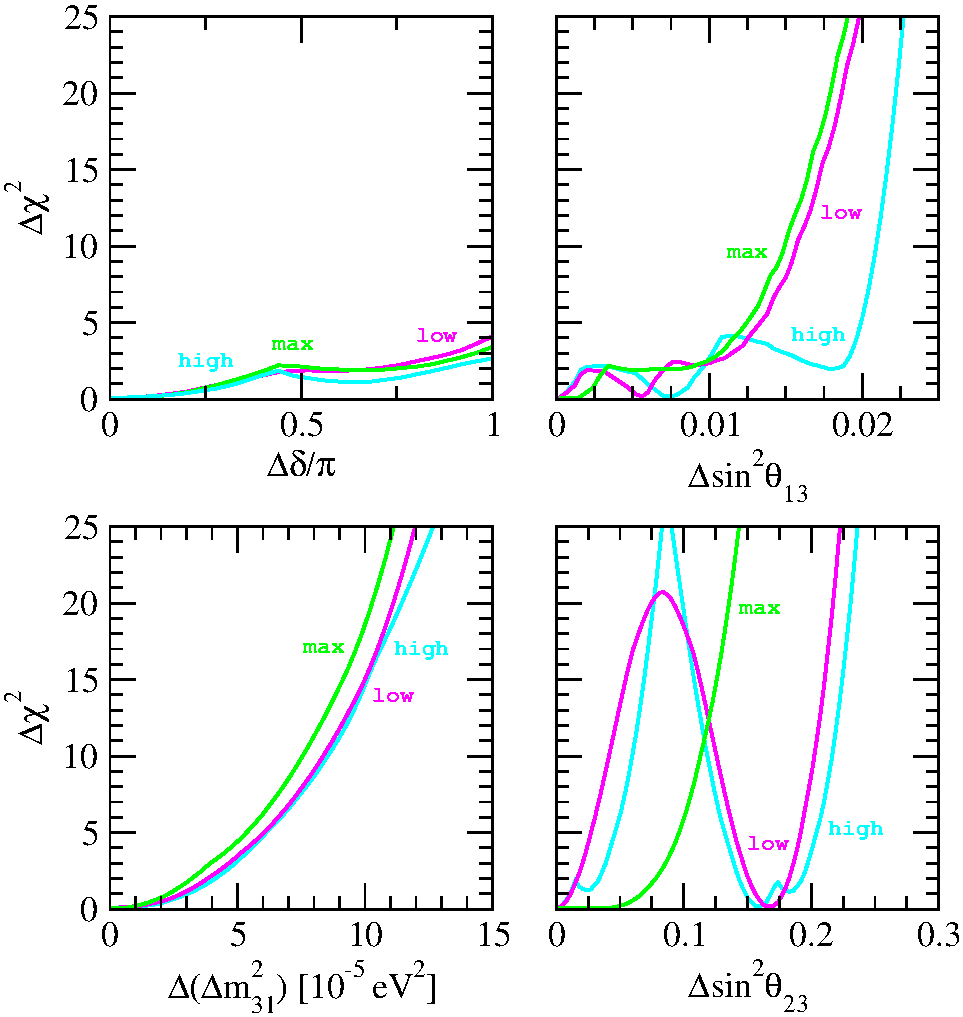
\includegraphics[width=0.55\columnwidth]{graphics/sensitivity-CPT.pdf}
        \caption{The sensitivities of DUNE to the difference of neutrino and antineutrino parameters: 
        $\Delta\delta$, $\Delta(\Delta m_{31}^2)$, $\Delta(\sin^2\theta_{13})$ and $\Delta(\sin^2\theta_{23})$  
        for the atmospheric angle in the lower octant (magenta line),  in the upper octant (cyan line) and for maximal mixing (green line).}
	\label{fig:sensitivity-CPT}
\end{figure}

\subsubsection{Imposter solutions}
\label{sec:impost}
In different types of neutrino oscillation experiments, as for example accelerators, neutrino and antineutrino data are obtained in separate experimental runs. However, the usual procedure followed by the experimental collaborations, as well as the global oscillation fits as for example ref.~\cite{deSalas:2017kay}, assumes CPT invariance and analyzes the full data sample in a joint way. 
%
%Such a path is not risk-free. Indeed, the opportunity to test CPT invariance in the neutrino sector is lost. Even more importantly, 
However, if CPT is violated in nature, the outcome of the joint data analysis might give rise to what we call an imposter solution. A solution which results from the combined analysis but does not correspond to the true solution of any channel. 

Under the assumption of CPT conservation, the $\chi^2$--functions are computed according to
%
\begin{equation}
 \chi^2_{\text{total}}=\chi^2(\nu)+\chi^2(\overline{\nu})\, ,
 \label{eq:cpt-cons}
\end{equation}
%
and assuming that the same parameters describe neutrino and antineutrino flavor oscillations. In contrast, in Eq.~(\ref{eq:chi2-nu-nubar}) we first profiled over the parameters in neutrino and antineutrino mode separately and then added the profiles. Here, we shall assume CPT to be violated in nature, but perform our analysis as if it was conserved. As an example, we assume that the true value for the atmospheric neutrino mixing is $\sin^2\theta_{23}=0.5$, while the antineutrino mixing angle is given by $\sin^2\overline{\theta}_{23}=0.43$. The rest of the oscillation parameters are set to the values in table~\ref{tab:par2}. Performing the statistical analysis in the CPT conserving way, as indicated in Eq.~(\ref{eq:cpt-cons}), we obtain the profile of the atmospheric mixing angle presented in figure~\ref{fig:imposter-sq23}. The profiles for the individual reconstructed results (neutrino and antineutrino) are also shown in the figure for comparison.
%As can be seen, we obtain
The result is a new best fit value at $\sin^2\theta^\text{comb}_{23}=0.467$, disfavoring the true values for neutrino and antineutrino parameters at approximately 3$\sigma$ and more than 5$\sigma$, respectively. 

\begin{figure}[!htb]
 \centering
        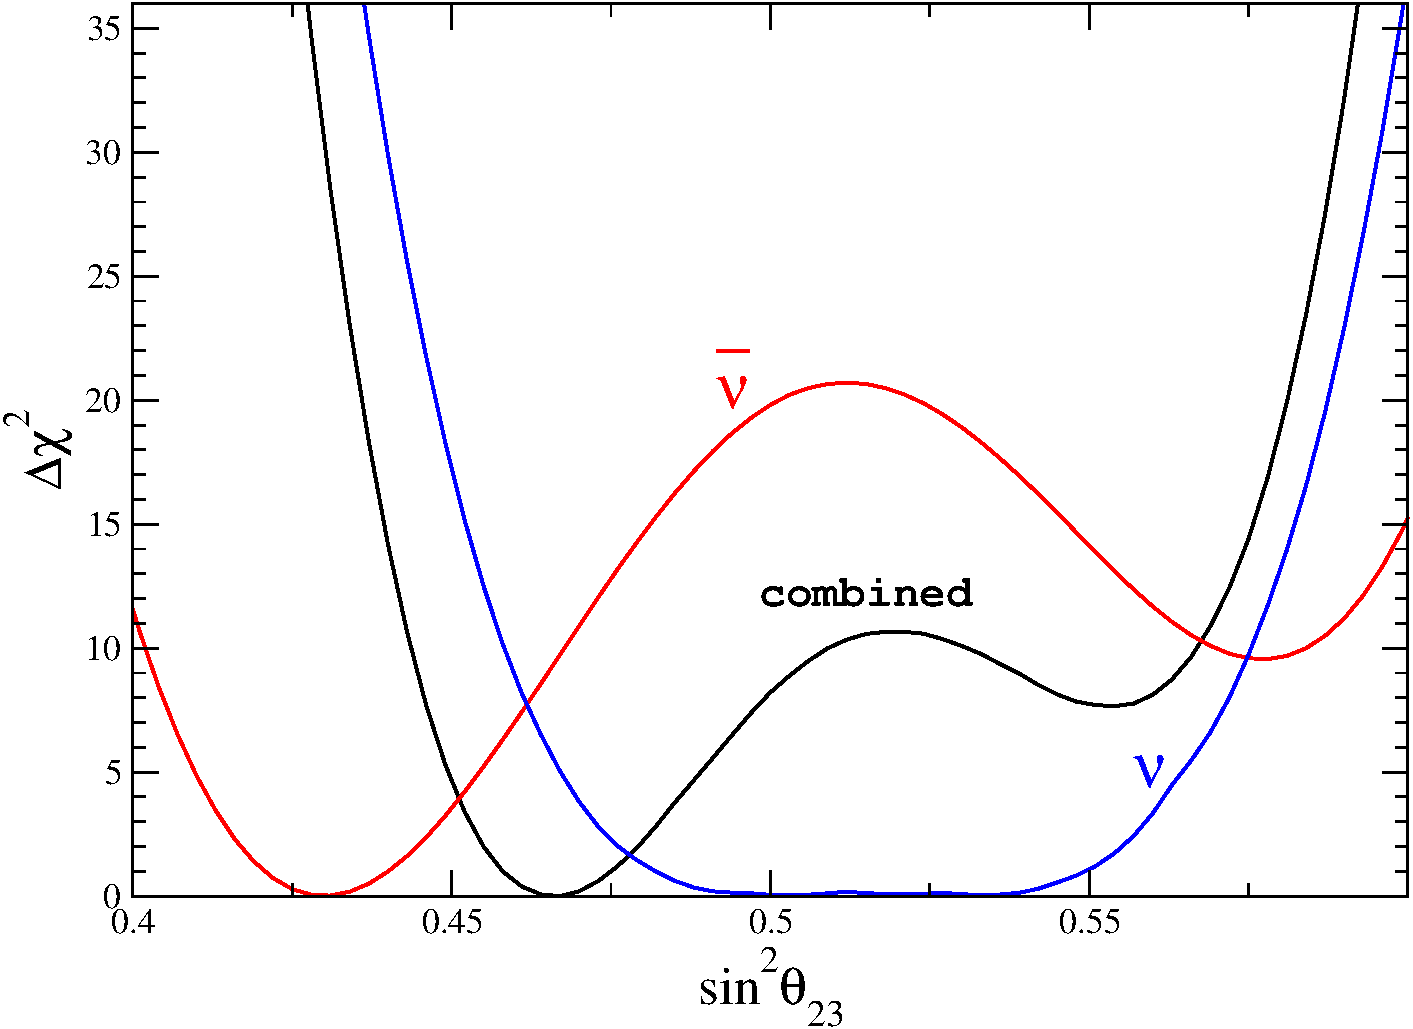
\includegraphics[width=0.6\columnwidth]{graphics/imposter-sq23.pdf}
        \caption{DUNE sensitivity to the atmospheric angle for neutrinos (blue), antineutrinos (red) and to the combination of both under the assumption of CPT conservation (black).
         }
	\label{fig:imposter-sq23}
\end{figure}

\section{Search for Boosted Dark Matter from the Sun}

\subsection{\label{sec:level1}Introduction}

Due to the increasingly stronger constraints on the long-standing paradigm of dark matter (DM), Weakly Interacting Massive Particles (WIMP), it is of utmost importance to expand the DM searches to include alternative candidates and non-minimal scenarios. A class of models called boosted dark matter (BDM) was first studied in \cite{Huang:2013xfa,Agashe:2014yua, Berger:2014sqa}, leading to the novel phenomenology that a small non-thermal component of DM today is relativistic and effectively interacts with Standard Model (SM) particles, which can be the smoking-gun for DM discovery. This is in contrast to the conventional assumption that DM is composed of one particle species that is deeply non-relativistic. BDM originates from DM annihilation in a two-component dark sector or semi-annihilation in the original work, but can also generically arise from other scenarios \cite{Carlson:1992fn, Hochberg:2014dra,Huang:2013xfa}. 

Conventional DM direct detection is generally not suitable to capture the small flux of BDM that leads to energetic outgoing SM particles upon its scattering (for exception, see \cite{Cherry:2015oca, Cui:2017ytb}). On the other hand, large volume neutrino detectors stand out as natural, ideal facilities for such searches. The two interaction channels of BDM, with electrons \cite{Agashe:2014yua} and with hadrons (protons) \cite{Berger:2014sqa}, were investigated for Cherenkov detectors, such as Super-Kamiokande (Super-K) which recently published a dedicated search for BDM in electron channel \cite{Kachulis:2017nci}. However, in such detectors the BDM signal rate is shown to be often significantly attenuated due to Cherenkov threshold, in particular for hadronic channels. 

The recently developed Liquid Argon detectors, such as employed by DUNE, have the potential to greatly improve the sensitivity for BDM compared to Cherenkov detectors. This is due to improved particle identification techniques, as well as a significantly lower energy threshold for proton detection. Earlier studies have shown an improvement with DUNE for BDM-electron interaction \cite{Necib:2016aez}. In this work employing newly developed dedicated simulation tools, we demonstrate that DUNE can majorly expand the reach of SuperK when BDM scatters off protons.

Other studies of BDM models have examined sensitivity at DUNE and elsewhere~\cite{Agashe:2014yua,Berger:2014sqa,Alhazmi:2016qcs,Necib:2016aez,Kim:2016zjx,Kachulis:2017nci,Giudice:2017zke,Chatterjee:2018mej,Kim:2018veo}. The hadronic interaction model presented here is complementary to other model studies. This study is the first to study such a model at DUNE with full event generation and detector simulation.

\subsection{\label{sec:level2}Theory Discussion}
In the remainder of this study, we focus on the example of BDM arising from a two-component dark sector as studied in \cite{Agashe:2014yua, Berger:2014sqa}. This scenario consists of two stable dark particles, $\psi$ and $\chi$, specified as fermions in this study. Particle $\psi$ is more massive than $\chi$, and is the dominant DM today with its abundance determined by thermal annihilation of $\psi\psi\rightarrow\chi\chi$. The present-day annihilation of $\psi$ leads to BDM $\chi$ with a boost factor of $\gamma = m_\psi/m_\chi$. The BDM-SM interaction may proceed via exchange of a dark photon $\gamma'$ or $Z'$.

In this work we focus on BDM flux sourced by DM annihilation in the core of the Sun. DM particles can be captured by the Sun through their scattering with the nuclei in the Sun, mostly Hydrogen and Helium. This makes the core of the Sun a region with concentrated DM distribution. The BDM flux is
\begin{eqnarray} \label{eq:flux}
\Phi= f \frac{A}{4\pi D^2},
\end{eqnarray}
where $A$ is the annihilation rate, and $D = 1\,\rm{AU}$ is the distance from the Sun. $f$ is a model-dependent parameter, where $f = 2$ for two-component DM as considered here.

For the parameter space we are interested in, assuming DM annihilation cross section is not too small, the DM distribution in the Sun has reached an equilibrium between capture and annihilation. This helps to eliminate the annihilation cross section dependence in our study.

Two additional comments are in order. First, the DM particles cannot be too light, i.e.\ lighter than 4\,GeV \cite{Griest:1986yu,Gould:1987ju}, or else we will lose most of the captured DM through evaporation rather than annihilation, which would dramatically reduce the BDM flux. Additionally, one needs to check that BDM particles cannot lose energy and potentially be recaptured by scattering with the solar material when they escape from the core region after production. Rescattering is found to be rare for the benchmark models considered in this study and we consider the BDM flux to be monochromatic at its production energy.

The event rate to be observed at DUNE is 
\begin{equation}
R = \Phi \times \sigma_{\rm{SM} - \chi} \times \epsilon \times N,
\end{equation}
 where $\Phi$ is the flux given by Eq. \ref{eq:flux}, $\sigma_{\rm{SM} - \chi}$ is the scattering cross section of the BDM off of SM particles, $\epsilon$ is the efficiency of the detection of such a process, and $N$ is the number of target particles in DUNE. The computation of the flux of BDM from the Sun can be found in Ref. \cite{Berger:2014sqa}. 
 
We generate the signal events and calculate interaction cross-sections in the detector using a newly developed boosted dark matter module\cite{Andreopoulos:2009rq,Andreopoulos:2015wxa,Berger:2018}, which includes elastic and deep inelastic scattering, as well as a range of nuclear effects. This conservative event generation neglects the dominant contributions from baryon resonances in the final state hadronic invariant mass range of 1.2 to 1.8 GeV, which should not have a major effect on our main results. The interactions are taken to be mediated by an axial, flavor universal $Z^\prime$ coupling to both the BDM and with the quarks. The axial charge is taken to be 1. 
% The resulting cross-sections with argon are shown in Tab.~\ref{tab:eff-tab}. 
The events are generated for the 10\,kton DUNE detector~\cite{dunetpc_code}, though we only study the dominant scattering off of the ${}^{40}{\rm Ar}$ atoms therein. The method for determining the efficiency $\epsilon$ is described below. The number of target Argon atoms is $N = 1.5  \times 10^{32}$ assuming a target mass of 10\,kton.

% -------------------------------------------------------------------------------
\subsection{Background Estimation}
\label{sec:background}

The main background in this process comes from the neutral-current (NC) 
interactions of atmospheric neutrinos and Argon,
as they share the features that the timing of events is unknown in advance,
and that the interactions with Argon produce hadronic activity in the detector.
We use GENIE\cite{Andreopoulos:2009rq,Andreopoulos:2015wxa}
interfaced by the LArSoft toolkit to generate the NC atmospheric
neutrino events, and obtain 845 events in a 10\,kton module for one year of
exposure.

% -------------------------------------------------------------------------------

\subsection{Detector Response}
\label{sec:detector_resp}

The finite detector resolution is taken into
account by smearing the direction of the stable final state particles, 
including protons, neutrons, charged pions, muons, electrons, and photons,
with the expected angular resolution,
and by ignoring the ones with kinetic energy below detector threshold,
using the parameters reported in DUNE conceptual design report (CDR)~\cite{DUNE_CDR_V2}.
We form as the observable the total momentum from all the stable final state particles,
and obtain its angle with respect to the direction of the Sun.
The Sun position is simulated with the SolTrack package~\cite{SolTrack}
including the geographical coordinates of the DUNE far detector~\cite{DUNE_DocDB136}.
We consider both the scenarios where we can reconstruct neutrons and where
neutrons will not be reconstructed.
Fig.~\ref{fig:m10_SmearedReconstructableAngle} shows the angular distributions of
the BDM signals with mass of 10\,GeV and different boost factors,
and of the background events.

% ---------------------------------------------------------------------------------
\begin{figure*}[!htb]
\centering
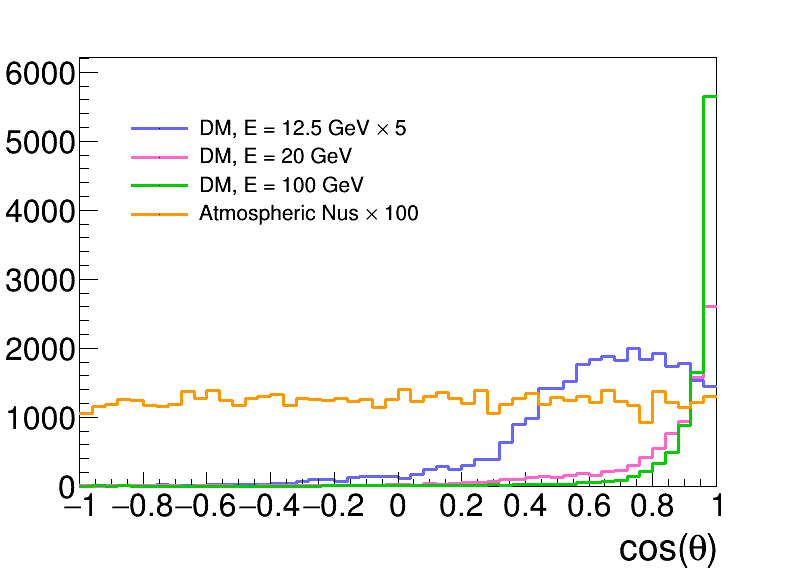
\includegraphics[width=0.45\textwidth]{graphics/m10_SmearedReconstructableAngle.png}
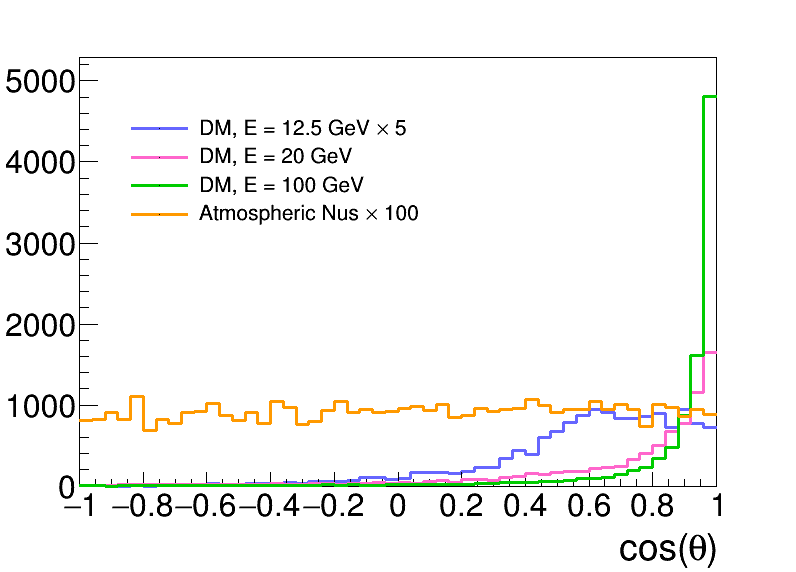
\includegraphics[width=0.45\textwidth]{graphics/m10_SmearedReconstructableNoNAngle.png}
\caption{Angular distribution of the BDM signal events with the BDM mass of 10\,GeV
and different boosted factors, $\gamma$, and of the atmospheric neutrino NC
background events.
$\theta$ represents the angle of the sum over all the stable final state
particles as detailed in the text.
The amount of background represents one-year data collection, magnified by a factor 100,
while the amount of signal reflects the detection efficiency of 10,000 MC events, as
described in this note.
The left plot shows the scenario where neutrons can be reconstructed,
while the right plot represents the scenario without neutrons.}
\label{fig:m10_SmearedReconstructableAngle}
\end{figure*}
% ---------------------------------------------------------------------------------


To increase the signal fraction in our samples, we select events with $\cos\theta > 0.6$,
and obtain the selection efficiency $\epsilon$ for different BDM models.
% as listed in Table~\ref{tab:eff-tab}, 
$104.0 \pm 0.7$ and $79.4 \pm 0.6$ background events per year, in the scenarios with and without neutrons respectively,
survive the selection in a DUNE 10\,kton module.

\subsection{Results}

\begin{figure*}[!htb]
\centering
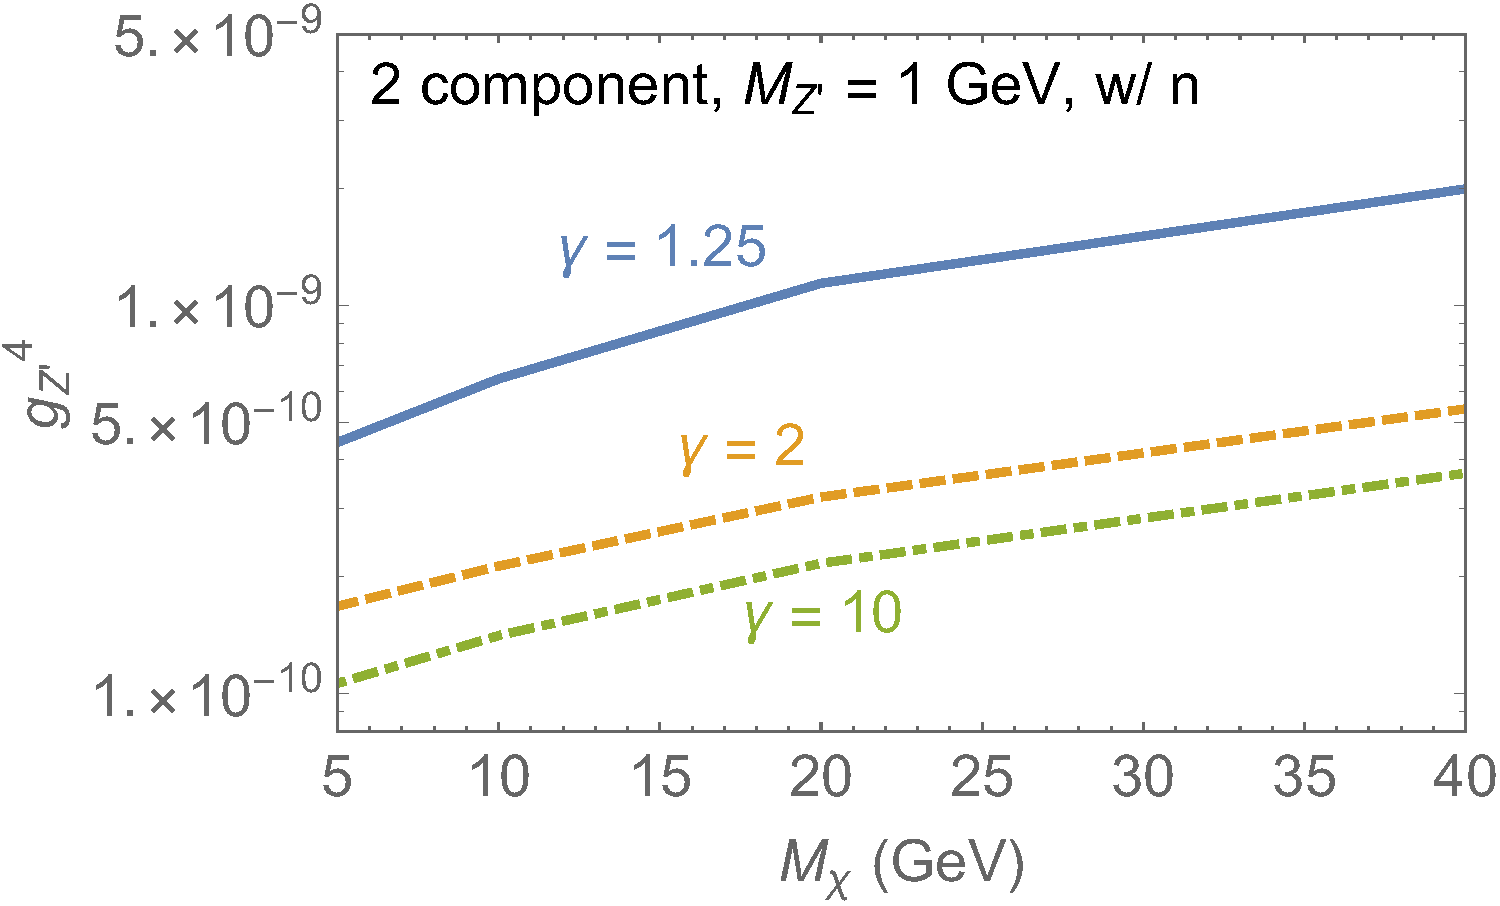
\includegraphics[width=0.45\textwidth]{graphics/expected-discovery-with-n.pdf}\hspace{0.05\textwidth}
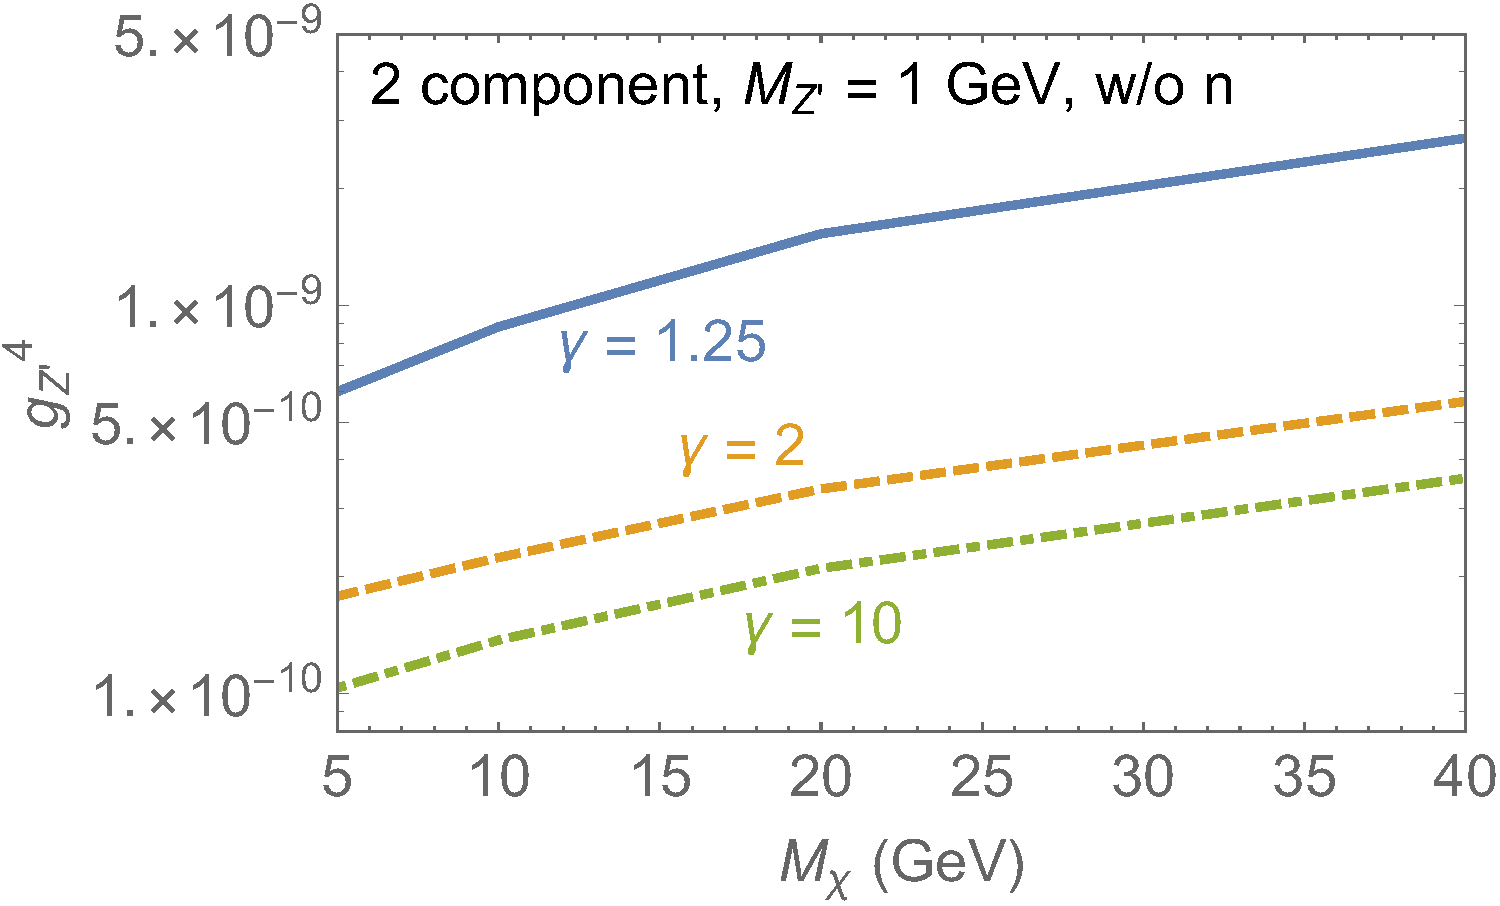
\includegraphics[width=0.45\textwidth]{graphics/expected-discovery-no-n.pdf}
\caption{Expected $5\sigma$ discovery reach with 1 year of DUNE livetime including neutrons in reconstruction (left) and excluding neutrons (right).\label{fig:significance}}
\end{figure*}
The resulting expected sensitivity is presented in Fig.~\ref{fig:significance} in terms of the dark matter mass and the $Z^\prime$ gauge coupling for potential DM boosts of $\gamma = 1.25,2,10$ and for a fixed mediator mass of $m_{Z^\prime} = 1~{\rm GeV}$.  We assume a DUNE livetime of 1 year.  The models presented here are currently unconstrained by direct detection searches if the thermal relic abundance of the DM is chosen to fit current observations.

\subsection{Conclusions}

BDM is motivated by a variety of non-minimal dark sector scenarios that has gained increasing interest in recent years. Thanks to its relatively low threshold and strong particle identification capabilities, DUNE presents an opportunity to significantly advance the search BDM beyond what has been possible with water Cherenkov detectors. With 1 year of data, the $5\sigma$ sensitivity is expected to reach a coupling of $g_{Z^\prime}^4 = 9.57 \times 10^{-10}$ for a boost of 1.25 and $g_{Z^\prime}^4 = 1.49 \times 10^{-10}$ for a boost of 10 at a DM mass of 10 GeV without including neutrons in the reconstruction.


\section{Other BSM Physics Opportunities}

\subsection{Tau neutrino appearance} The tau neutrino was not directly observed until 2000 by the DONuT experiment, which used emulsion technology to detect  $\nu_{\tau}$-CC and $\bar{\nu}_{\tau}$-CC produced by $D_S$ meson decays originating from an 800 GeV proton beam stopped by a tungsten alloy beam dump.  A total of 9 $\nu_{\tau}$-CC and $\bar{\nu}_{\tau}$-CC candidate events were observed with an estimated background of 1.5 events~\cite{Kodama:2000mp, Kodama:2007aa}.

The OPERA experiment was also designed with emulsion technology to discover tau neutrino appearance in a muon neutrino beam~\cite{Guler:2000bd}. OPERA succeeded in discovering tau neutrino appearance~\cite{Agafonova:2015jxn}; however, the baseline and energy of the experiment was such that appearance was suppressed by a factor of 0.01.   The final analysis identified 10 $\nu_{\tau}$-CC candidate events with an estimated background of 2 events.  From this sample, a 20\% measurement of $\Delta m^{2}_{32}$ was performed under the assumption that $\sin^22\theta_{23} = 1$~\cite{Agafonova:2018auq}.  Super-Kamiokande has developed a method to statistically separate a sample of $\nu_{\tau}$-CC and $\bar{\nu}_{\tau}$-CC events in atmospheric neutrinos to exclude the no-tau-neutrino appearance hypothesis at the 4.6$\sigma$ level~\cite{Abe:2012jj, Li:2017dbe}, but limitations of water Cherenkov detectors limit the ability to select a high purity sample and perform precision measurements.

With only 19 $\nu_{\tau}$-CC and $\bar{\nu}_{\tau}$-CC candidates detected with high purity, we have less direct experimental knowledge of tau neutrinos than any other Standard Model particle. Our knowledge of the tau-neutrino cross-section is inferred from measurements of muon neutrinos assuming lepton universality, such that any cross-section differences are only due to the large mass of the tau lepton. However, recent data from Belle, BaBar, and LHCb, as combined by the Heavy Flavor Averaging Group, shows that certain decays involving tau leptons differ from Standard Model predictions assuming lepton universality by 3.9$\sigma$~\cite{Amhis:2016xyh}.  This anomaly could be explained with a $W'$-boson~\cite{Greljo:2018ogz}, which could potentially induce NSI affecting $\nu_{\tau}$ appearance.  Similarly, almost all knowledge of the tau-neutrino mixing-matrix elements comes from assuming unitarity of the mixing matrix. Without assuming unitarity, one critical element is only known to 60\%~\cite{Parke:2015goa}.

The DUNE experiment has the possibility of significantly improving the experimental situation.  Tau-neutrino appearance can potentially improve the discovery potential for sterile neutrinos, NSI, and non-unitarity.  For model independence, the first goal should be measuring the atmospheric oscillation parameters in the $\nu_{\tau}$ appearance channel and checking the consistency of this measurement with those performed using the $\nu_{\mu}$ disappearance channel.  A truth-level study of $\nu_{\tau}$ selection in atmospheric neutrinos in a large, underground LArTPC detector suggested that $\nu_{\tau}$-CC interactions with hadronically decaying $\tau$-leptons, which make up 65\% of total $\tau$-lepton decays~\cite{PDG}, can be selected with high purity~\cite{Conrad:1008}.  This analysis suggests that it may be possible to select up to 29\% of $\nu_{\tau}$-CC events with hadronically decaying $\tau$-leptons with minimal neutral current background.  Under these assumptions, we expect to select $\sim$25 $\nu_{\tau}$-CC candidates per year using the CP-violation optimized beam.  This is sufficient to be able to simultaneously constrain $\Delta m^2_{31}$ and $\sin^22\theta_{23}$; however, all of these events occur at energies higher than the first oscillation maximum due to kinematic constraints.  Only seeing the tail of the oscillation maximum creates a partial degeneracy between the measurement of  $\Delta m^2_{31}$ and $\sin^22\theta_{23}$.  Atmospheric neutrinos, due to sampling a much larger $L/E$ range, allow for measuring both above and below the first oscillation maximum with $\nu_{\tau}$ appearance.  Although the we only expect to select $\sim$70 $\nu_{\tau}$-CC and $\bar{\nu}_{\tau}$-CC candidates in 350 kt-year in the atmospheric sample,  a direct measurement of the oscillation maximum should break the degeneracy seen in the beam sample.  Finally, a high-energy beam option optimized for $\nu_{\tau}$ appearance should produce $\sim$150 selected  $\nu_{\tau}$-CC candidates in one year.  These higher energy events are further in the tail of the first oscillation maximum, but they will permit a simultaneous measurement of the $\nu_{\tau}$ cross-section. 

\subsection{Heavy Neutral Leptons}
The high intensity of the LBNF neutrino beam and the production of charm and bottom mesons in the beam enables DUNE to search for a wide variety of lightweight long-lived, exotic particles, by looking for topologies of rare event interactions and decays in the fiducial volume of the DUNE near detector. These particles include weakly-interacting heavy neutral leptons – right-handed partners of the active neutrinos, vector, scalar, or axion portals to the Hidden Sector, and light super-symmetric particles. Assuming these heavy neutral leptons are the lighter particles of their hidden sector, they will only decay into standard model particles. The parameter space explored by the DUNE near detector extends into the cosmologically relevant region complementary to the LHC heavy-mass dark-matter searches through missing energy and mono-jets.

\subsection{Large Extra Dimensions}
DUNE can search for or constrain the size of large extra-dimensions (LED) by looking for distortions of the oscillation pattern predicted by the three-flavor paradigm. These distortions arise through mixing between the right-handed neutrino Kaluza-Klein modes, which propagate in the compactified extra dimensions, and the active neutrinos, which exist only in the four-dimensional brane [48]. Searching for these distortions in, for instance, the $\nu_{\mu}$ CC disappearance spectrum should provide significantly enhanced sensitivity over existing results from the MINOS/MINOS+ experiment [49].

\subsection{Dark Matter Annihilation in the Sun}
DUNE's large Far Detector LArTPC modules provide an excellent setting to conduct searches for neutrinos arising from dark matter annihilation in the core of the Sun. These would typically result in a high-energy neutrino signal almost always accompanied by a low-energy neutrino component, which has its origin in a hadronic cascade that
develops in the dense solar medium and produces large numbers of light long-lived mesons, such as $\pi^+$ and $K^+$, which will then stop and decay at rest. The decay of each $\pi^+$ and $K^+$ will
produce monoenergetic neutrinos with an energy 30 MeV or 236 MeV, respectively.
The 236 MeV flux can be measured with the DUNE Far Detectors, thanks to its excellent energy resolution, and importantly, will benefit from directional information. By selecting neutrinos arriving from the direction of the Sun, large reduction in backgrounds can be achieved.
This directional resolution for sub-GeV neutrinos will enable DUNE to be competitive with experiments with even larger fiducial masses, but less precise angular information, such as Hyper-K~\cite{ref:DMannihilation}.

\section{Conclusions and Outlook}
The DUNE Experiment will be a powerful discovery tool on a variety of physics topics under very active exploration today, from the potential discovery of new particules beyond those predicted in the Standard model, to precision neutrino measurements that may uncover deviations from the present three-flavor mixing paradigm and unveil new interactions and symmetries.
The Near Detector alone will offer excellent opportunities to search for light dark matter and mixing with light sterile neutrinos, and to measure rare processes such as neutrino trident interactions. Besides looking for deviations from the three-flavor oscillation paradigm such as nonstandard interaction, DUNE's massive high-resolution Far Detector will probe  the possible existence of boosted dark matter. The flexibility of the LBNF beamline enables planning for high-energy beam running, providing access to probing and measuring tau neutrino physics with unprecedented precision.

DUNE will offer a long-term privileged setting for collaboration between experimentalist and theorists in the domain areas of neutrino physics, astrophysics, and cosmology, and will provide the highest potential for breakthrough discoveries among the new near-term facilities projected to start operations during the next decade.


%%%%%%%%%%%%%%%%%%%%%%%%%%%%%%%%%%%%%%%%%%%%%%%%%%%%%%%%%%%%%%
% \section{Beam-induced physics capitalizing on DUNE far detector capabilities}\label{sec:bsm-beam}

% \begin{itemize}
% \item General Motivation
% \item Summary of Difference in Assumptions from Standard Oscillations if applicable (e.g. Det. Geometry, Flux, systematics)
% \item Common Software Tools
% \end{itemize}

% \subsection{Light Sterile Neutrinos}
% \begin{itemize}
% \item Motivation
% \item Datasets, signal, background studies
% \item List of Key Plots/tables
% \item Results and Conclusions
% \end{itemize}
% Experimental results in tension with the three-neutrino-flavor paradigm~\cite{LSNDSterile,MiniBooNESterile,GalliumSummary,ReactorSummary}, which may be interpreted as mixing between the known active neutrinos and one or more {\it sterile} states, have led to a rich and diverse program of searches for oscillations into sterile neutrinos.
% DUNE is sensitive over a broad range of potential sterile neutrino mass splittings by looking for disappearance of CC and NC interactions over the long baseline separating the near and far detectors, as well as over the short baseline of the near detector. 
% %Results from the MINOS and NOvA long-baseline accelerator experiments~\cite{MINOSSterile2016, NOvASterile2017} have demonstrated the validity of this approach. 
% With a longer baseline, a more intense beam, and a high-resolution large-mass far detector, compared to previous experiments, DUNE provides a unique opportunity to improve significantly on the sensitivities of the existing probes, and greatly enhance the ability to map the extended parameter space if a sterile neutrino is discovered.

% Assuming a 3+1 scenario, with a new squared mass splitting $\Delta m^2_{41}$, with the unitary PMNS mixing matrix augmented with one sterile state, the relevant oscillation probabilities for DUNE as a function of L/E and neutrino energy for different values of $\Delta m^2_{41}$ are shown in Fig.~\ref{fig:LoverE}. 
% \begin{figure}[!htbp]
% %\includegraphics[width=0.49\columnwidth]{./figures/DUNE_SterileSensi_dm0_05}
% %\includegraphics[width=0.49\columnwidth]{./figures/DUNE_SterileSensi_dm5}
% \caption{\label{fig:LoverE} Oscillation probabilities as a function of L/E and neutrino energy for different values of $\Delta m^2_{41}$. For values of $\Delta m^2_{41} > 1\,\mathrm{eV}^2$, distortions occur at the ND baseline, spanning the L/E range probed by LSND and MiniBooNE.}
% \end{figure}

% Assessment of DUNE's sensitivity to mixing with light sterile neutrinos proceeds through a simultaneous ND and FD fit framework developed with GLoBES~\cite{ref:globes}.
% The obtained sensitivities for the various mixing angles are shown in Figs.~\ref{fig:th_24}, \ref{fig:th_mue}, \ref{fig:th_14}, \ref{fig:th_34}. 

% \begin{figure}[!htbp]
% \centering
% %\includegraphics[width=0.5\columnwidth]{./figures/MultiPlots_DUNE_MINOS_IceCube_globAppF_th_24}
% \caption{\label{fig:th_24} DUNE 95\% C.L. limit on $\sin^2 \theta_{24}$ compared to current and previous experiments.}
% \end{figure}

% \begin{figure}[!htbp]
% \centering
% %\includegraphics[width=0.5\columnwidth]{./figures/DUNE_ComboLimit95_th_mue}
% \caption{\label{fig:th_mue} DUNE 95\% C.L. limit on $\sin^2 \theta_{\mu e}$ compared to current and previous experiments.}
% \end{figure}

% \begin{figure}[!htbp]
% \centering
% %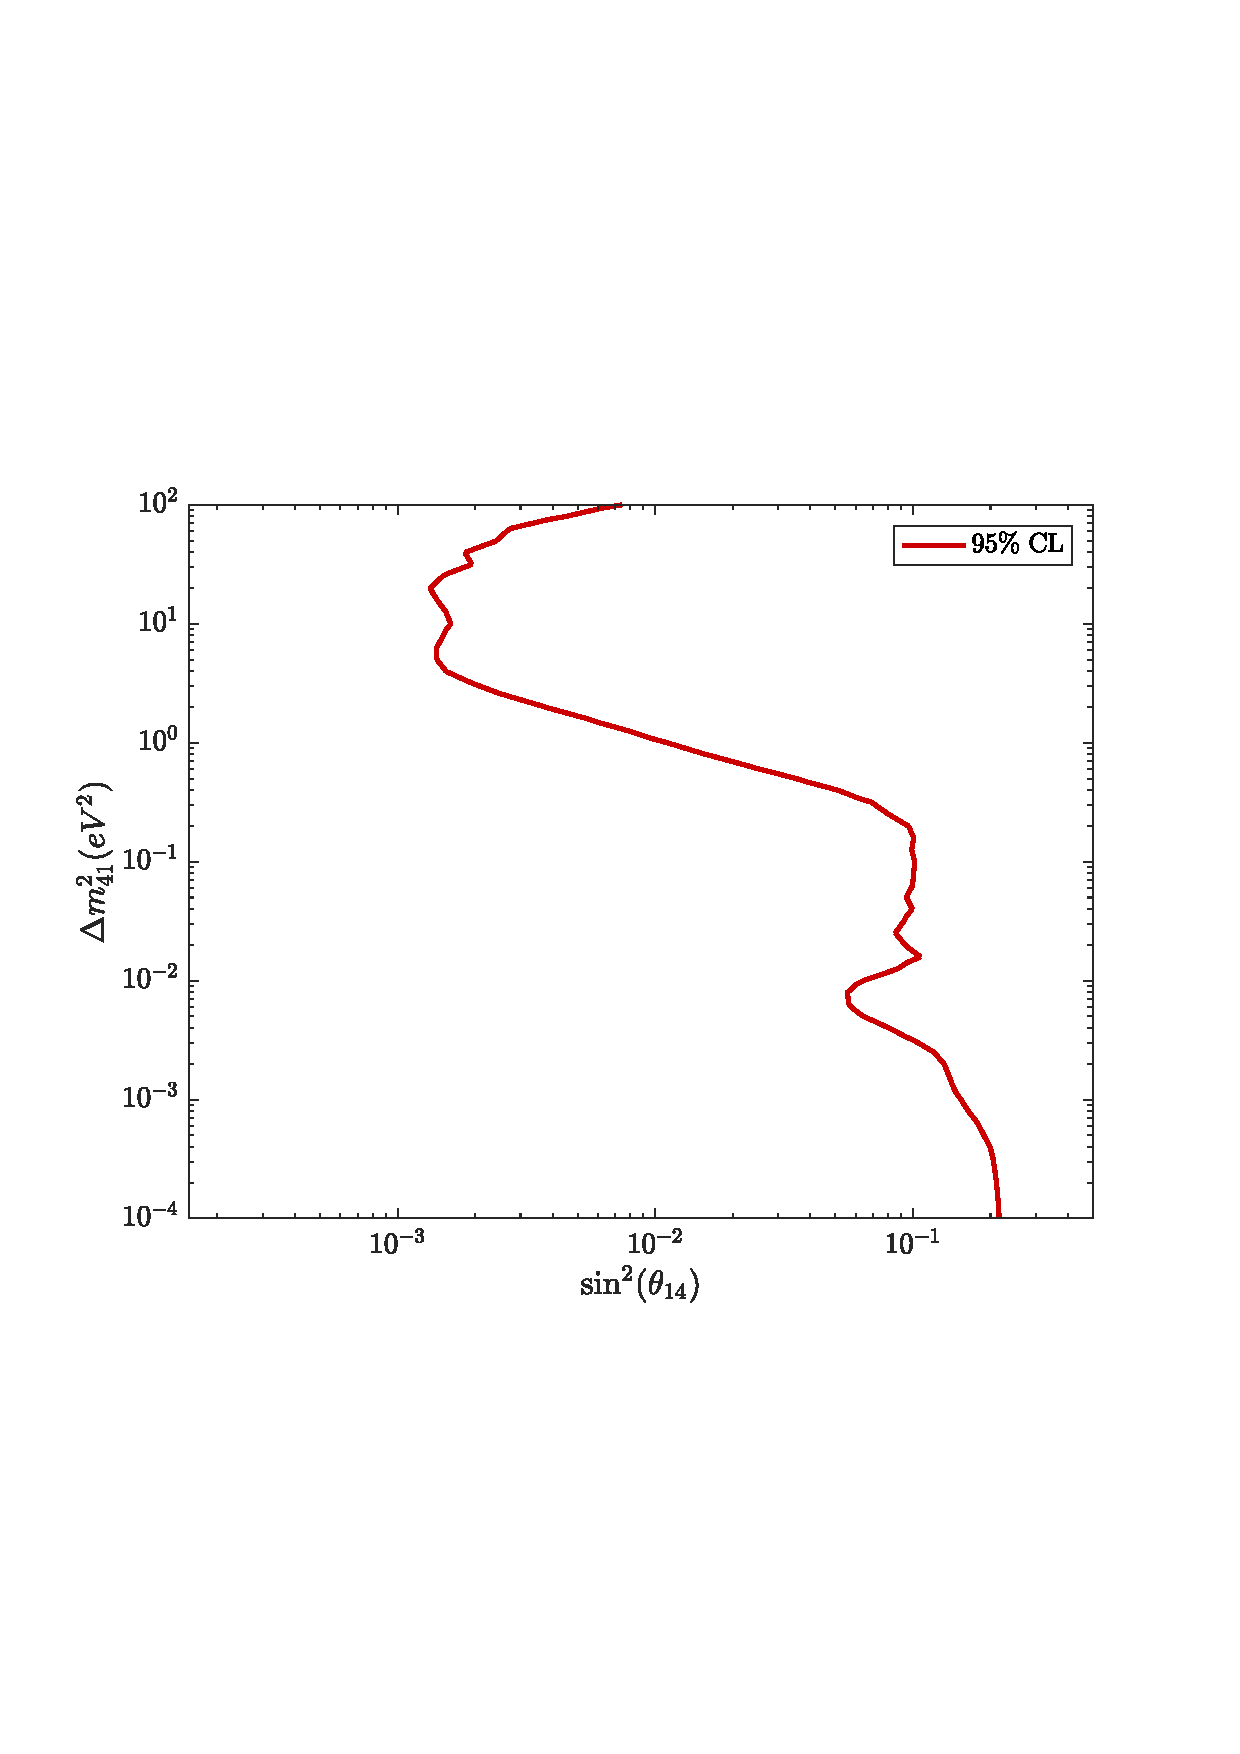
\includegraphics[width=0.4\columnwidth]{./figures/th_14}
% \caption{\label{fig:th_14} DUNE 95\% C.L. limit on $\sin^2 2\theta_{14}$ compared to current and previous experiments - placeholder.}
% \end{figure}

% \begin{figure}[!htbp]
% \centering
% %\includegraphics[width=0.4\columnwidth]{./figures/th_34}
% \caption{\label{fig:th_34} DUNE 95\% C.L. limit on $\sin^2 \theta_{34}$ compared to current experiments - placeholder.}
% \end{figure}

% \subsection{Large Extra-Dimensions}
% \begin{itemize}
% \item Motivation
% \item Datasets, signal, background studies
% \item List of Key Plots/tables
% \item Results and Conclusions
% \end{itemize}
% DUNE can search for or constrain the size of large extra-dimensions (LED) by looking for distortions of the oscillation pattern predicted by the three-flavor paradigm. These distortions arise through mixing between the right-handed neutrino Kaluza-Klein modes, which propagate in the compactified extra dimensions, and the active neutrinos, which exist only in the four-dimensional brane~\cite{LEDModel}. Searching for these distortions in, for instance, the $\nu_\mu$~CC disappearance spectrum should provide significantly enhanced sensitivity over existing results from the MINOS/MINOS+ experiment~\cite{MinosplusLED}.


% \subsection{Non-Standard Neutrino Interactions}
% \begin{itemize}
% \item Motivation
% \item Datasets, signal, background studies
% \item List of Key Plots/tables
% \item Results and Conclusions
% \end{itemize}

% \subsection{Non-Unitary Mixing}
% \begin{itemize}
% \item Motivation
% \item Datasets, signal, background studies
% \item List of Key Plots/tables
% \item Results and Conclusions
% \end{itemize}

% \subsection{Anomalous Long-Baseline $\nu_{\tau}$ Appearance }
% \begin{itemize}
% \item Motivation
% \item Datasets, signal, background studies
% \item List of Key Plots/tables
% \item Results and Conclusions
% \end{itemize}

% \subsection{CPT Violation}
% \begin{itemize}
% \item Motivation
% \item Datasets, signal, background studies
% \item List of Key Plots/tables
% \item Results and Conclusions
% \end{itemize}






% %%%%%%%%%%%%%%%%%%%%%%%%%%%%%%%%%%%%%%%%%%%%%%%%%%%%%%%%%%%%%%
% \section{Non-accelerator physics capitalizing on DUNE far detector capabilities}\label{sec:bsm-nonaccel}
% \begin{itemize}
% \item General Motivation
% \item Software Tools
% \end{itemize}

% \subsection{Boosted Dark Matter}
% \begin{itemize}
% \item Motivation
% \item Datasets, signal, background studies
% \item List of Key Plots/tables
% \item Results and Conclusions
% \end{itemize}

% %%%%%%%%%%%%%%%%%%%%%%%%%%%%%%%%%%%%%%%%%%%%%%%%%%%%%%%%%%%%%%
% \section{BSM physics opportunities with the near detector}\label{sec:bsm-nd}
% \begin{itemize}
% \item General Motivation
% \item Near detector assumptions
% \item Software Tools
% \end{itemize}

% \subsection{Low-Mass Dark Matter}
% \begin{itemize}
% \item Motivation
% \item Datasets, signal, background studies
% \item List of Key Plots/tables
% \item Results and Conclusions
% \end{itemize}

% \subsection{Heavy Neutral Leptons}
% \begin{itemize}
% \item Motivation
% \item Datasets, signal, background studies
% \item List of Key Plots/tables
% \item Results and Conclusions
% \end{itemize}

% \subsection{Neutrino Tridents}
% \begin{itemize}
% \item Motivation
% \item Datasets, signal, background studies
% \item List of Key Plots/tables
% \item Results and Conclusions
% \end{itemize}
% The intriguing possibility that neutrinos may be charged under new gauge symmetries beyond the Standard Model (SM) $SU(3)_c\times SU(2)_L\times U(1)_Y$, and interact with the corresponding new gauge bosons can be tested with unprecedented precision by DUNE through near detector measurements of neutrino-induced di-lepton production in the Coulomb field of a heavy nucleus, also known as {\it neutrino trident} interactions~\cite{Altmannshofer:2014pba}. Although this process is extremely rare (SM rates are suppressed by a factor of $\sim 10^{-5}-10^{-7}$ with respect to CC interactions), the CHARM-II collaboration \cite{Geiregat:1990gz} and the CCFR collaboration \cite{Mishra:1991bv} both reported detection of several trident events ($\sim 40$ events at CCFR) and quoted cross-sections in good agreement with the SM predictions. With a predicted annual rate of over 100 di-muon neutrino trident interactions at the near detector, DUNE will be able to measure deviations from the SM rates and test for the presence of new gauge symmetries.

% \subsection{Short-Baseline Sterile Neutrino Mixing}
% \begin{itemize}
% \item Motivation
% \item Datasets, signal, background studies
% \item List of Key Plots/tables
% \item Results and Conclusions
% \end{itemize}
